\documentclass[twoside]{article}
\usepackage{booktabs}
\usepackage{arydshln}
\usepackage{placeins}
\usepackage{sectsty}
\usepackage{geometry}
\usepackage{fontawesome}
\usepackage{xcolor}
\usepackage{array}
\usepackage{float}
\usepackage{url}
\usepackage{ulem}
\usepackage{soul}
\usepackage{enumitem}
\usepackage{amsmath}
\usepackage{amsfonts}
\usepackage{titlesec}
\usepackage{amssymb}
\usepackage{fancyhdr}
\usepackage{setspace}
\usepackage[italian]{babel}
\usepackage{graphicx}
\usepackage{caption}
\usepackage{subcaption}
\usepackage{titling}
\usepackage{tikz}
\usetikzlibrary{shapes.geometric, arrows.meta, positioning, calc, fit, backgrounds}
\usepackage{varwidth}
\usepackage{datetime2}
\usepackage[numbers]{natbib}
\usepackage{graphicx}
\usepackage{hyperref}
\usepackage{tocloft}
\usepackage[linesnumbered,ruled,vlined]{algorithm2e}
\usepackage{amsmath}
\usepackage{amsfonts}

% Definizione di un colore viola scuro
\definecolor{darkviolet}{rgb}{0.5, 0.0, 0.5}

% per bibliografia
\usepackage{etoolbox}
\makeatletter
\renewcommand{\bibsection}{%
  \section*{\LARGE Bibliografia}%
  \@mkboth{\MakeUppercase{\refname}}{\MakeUppercase{\refname}}%
}
\makeatother


\renewcommand{\cftsecfont}{\boldmath\LARGE}
\renewcommand{\cftsubsecfont}{\boldmath\large}
\renewcommand{\cfttoctitlefont}{\LARGE\boldmath\bfseries} % Dimensione e stile del titolo dell'indice
\renewcommand{\cftsecfont}{\bfseries\boldmath\LARGE} % Sezioni principali con grassetto più forte
\renewcommand{\cftsubsecfont}{\large} % Sottosezioni non in grassetto

% aumenta spazio indice
\setlength{\cftbeforesecskip}{1.5em}  % Aumenta lo spazio prima di ogni sezione
\setlength{\cftbeforesubsecskip}{0.9em}  % Aumenta lo spazio prima di ogni sottosezione

% Modifica dimensioni delle sezioni
\titleformat{\section}
  {\fontsize{28}{30}\selectfont\bfseries}
  {\thesection}{1em}{}

\titleformat{\subsection}
  {\fontsize{20}{22}\selectfont\bfseries}
  {\thesubsection}{1em}{}

\titleformat{\subsubsection}
  {\fontsize{18}{20}\selectfont\bfseries}
  {\thesubsubsection}{1em}{}

\setstretch{1.2} % Regola lo spaziamento tra le righe dei paragrafi
\setlength{\parindent}{0pt} % Rimuove l'indentazione dei paragrafi

\geometry{
  a4paper,
  left=3.5cm,
  right=2.5cm,
  top=2.5cm,
  bottom=2.5cm,
  includeheadfoot,
  twoside
}

% Impostare i margini per le pagine dispari e pari
\ifodd\value{page}
  \geometry{left=3.5cm, right=2.5cm}
\else
  \geometry{left=2.5cm, right=3.5cm}
\fi

\hypersetup{
    linktoc=all,
    linkbordercolor=white, % Imposta il colore del bordo dei link a bianco
    colorlinks=true,
    linkcolor=black,
    urlcolor=cyan,
    citecolor=blue,
    pdftitle={Studio e simulazione di un'architettura 6G centralizzata per il tracking di droni indoor assistita da RIS},
}

\usepackage[utf8]{inputenc}
\usepackage{tcolorbox}
\tcbuselibrary{listingsutf8, breakable}

% Definizione dell'ambiente "code" per Python
\newtcblisting[auto counter, number within=section]{code}[2][]{
    colframe=gray!20, colback=gray!5, coltitle=black,
    listing only, breakable,
    listing options={
        basicstyle=\small\ttfamily, language=python, breaklines=true, tabsize=4, 
        numbers=left, numberstyle=\tiny\color{gray}, stepnumber=1, numbersep=5pt, 
        keywordstyle=\color{blue}\bfseries, commentstyle=\color{green!60!black}\ttfamily, 
        stringstyle=\color{red!60!black}, showstringspaces=false
    },
    title=\textbf{Snippet \thetcbcounter:} #2
}

\setlength{\parindent}{0pt}

% Impostazioni per pagine alternate
\pagestyle{fancy}
\fancyhf{}
\fancyfoot[LE,RO]{\thepage} % Numeri di pagina a sinistra sulle pagine pari e a destra sulle pagine dispari
\renewcommand{\headrulewidth}{0pt} % Rimuove la linea di intestazione
\renewcommand{\footrulewidth}{0pt} % Rimuove la linea di piè di pagina

% Impostazioni per la pagina dell'indice
\fancypagestyle{plain}{
    \fancyhf{}
    \fancyfoot[LE,RO]{\thepage} % Numeri di pagina a sinistra sulle pagine pari e a destra sulle pagine dispari
}

\begin{document}

%-----------------------------------------------------------
% TITLE-PAGE

\begin{titlepage}
\begin{figure}[H]
    \centering
    
\includegraphics[width=5cm]{Images/logo-unifi.png} % Assicurati che l'immagine sia nella cartella corretta
\end{figure}

\begin{center}
    {\fontsize{18}{20}\selectfont\textsc{Università degli Studi di Firenze}}\\
    \vspace{3mm}
    {\fontsize{12}{14}\selectfont\textsc{Scuola di Ingegneria - Dipartimento di Ingegneria \\dell'Informazione}}\\
    \vspace{4mm}
    \rule{55mm}{0.1mm}\\
    \vspace{4mm}
    {\fontsize{10}{12}\selectfont{Tesi di Laurea Triennale in Ingegneria Elettronica e delle Telecomunicazioni}}\\
\end{center}

\vspace{20mm}
\begin{center}
    {\LARGE{\bf{Studio e simulazione di un'architettura 6G centralizzata per il tracking di droni indoor assistita da RIS}}\\\vspace{5mm}}
\end{center}
\vspace{20mm}

\begin{minipage}[t]{0.47\textwidth}
	{\large{Relatore}{\normalsize\vspace{3mm}
	\bf\\ \large{Francesco Chiti}}}
\end{minipage}
\hfill
\begin{minipage}[t]{0.47\textwidth}\raggedleft
	{\large{Candidato}{\normalsize\vspace{3mm}
	\\ \large{\textbf{Matteo Verniani}}\\ \vspace{1.5mm} \large{N° matricola \\ \textbf{7052552}\vspace{2mm}}}}
\end{minipage}

\begin{center}
\vspace{10mm}
    {\fontsize{10}{12}\selectfont{Anno accademico 2025 / 2026}}
\end{center}

\thispagestyle{empty} % Nasconde il numero di pagina

\end{titlepage}

\newpage
\thispagestyle{empty}
\mbox{}
\clearpage

% Ripristina il normale stile delle pagine e imposta il contatore di pagina
\pagenumbering{arabic}
\setcounter{page}{3}

%------------------------------------------------------------------

\tableofcontents

\clearpage

\titleformat{\section}[display]
  {\normalfont\Large\bfseries}
  {}
  {0pt}
  {}
\titlespacing*{\section}
  {0pt}
  {0pt}
  {0pt}

\titleformat{\section}[hang]{\normalfont\Large\bfseries}{\thesection}{1em}{\raggedright}
\titleformat{\subsection}[hang]{\normalfont\large\bfseries}{\thesubsection}{1em}{\raggedright}



\titleformat{\section}[hang]{\normalfont\Large\bfseries}{\thesection}{1em}{\raggedright}
\titleformat{\subsection}[hang]{\normalfont\large\bfseries}{\thesubsection}{1em}{\raggedright}

\titleformat{\section}[hang]{\normalfont\Large\bfseries}{\thesection}{1em}{\raggedright}
\titleformat{\subsection}[hang]{\normalfont\large\bfseries}{\thesubsection}{1em}{\raggedright}
\titleformat{\subsubsection}[hang]{\normalfont\normalsize\bfseries}{\thesubsubsection}{1em}{\raggedright}

% Riduzione spazi equazioni
\setlength{\abovedisplayskip}{3pt}
\setlength{\belowdisplayskip}{3pt}
\setlength{\abovedisplayshortskip}{0pt}
\setlength{\belowdisplayshortskip}{0pt}

% -----------------------------------------------------------------

\section{Introduzione}

La transizione verso le reti cellulari di sesta generazione (6G) impone un ripensamento radicale delle architetture di telecomunicazione, evolvendo verso ecosistemi intelligenti capaci di supportare l'automazione robotica della Logistica 4.0 \cite{Yu2024,Zhang2022}. Il presente capitolo inquadra le severe sfide fisiche associate al tracciamento autonomo di flotte di UAV (Unmanned Aerial Vehicles) in ambienti industriali ad alta densità. Una delle criticità fondamentali è rappresentata dall'indisponibilità del segnale GPS in contesti indoor. L'assenza di un riferimento satellitare globale rende i sistemi di navigazione convenzionali totalmente inefficaci, delegando interamente alla rete radiomobile il compito di fornire sia la connettività che una stima posizionale estremamente precisa. Tuttavia, le imponenti infrastrutture metalliche tipiche dei magazzini intensivi (VNA - Very Narrow Aisle) generano un ambiente radiopropagativo ostile, dominato da condizioni di puro Non-Line-of-Sight (NLoS) e riflessioni caotiche che degradano drasticamente la qualità del segnale \cite{Ye2023,Gebretsadik2024}. 
\begin{figure}[H]
    \centering
    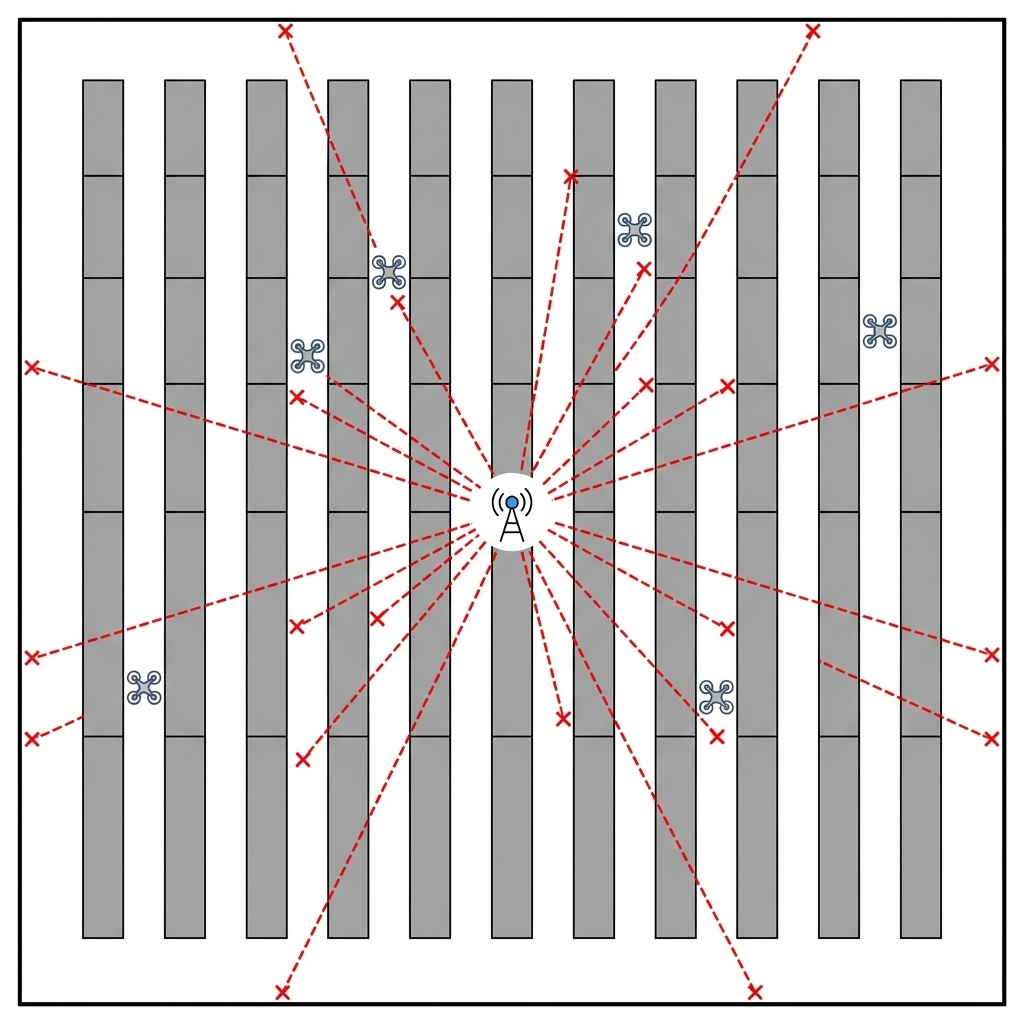
\includegraphics[width=0.35\textwidth]{../warehouse_drone_problem.png}
    \caption{Rappresentazione del limite operativo in un magazzino logistico VNA: totale ostruzione NLoS causata dalle scaffalature e negazione del tracciamento GPS (GPS-denied environment).}
    \label{fig:intro_problema}
\end{figure}

In questi scenari, definiamo tre obiettivi primari del lavoro per risolvere questi problemi:

\begin{itemize}
    \item Il raggiungimento di un tracking sub-metrico ininterrotto in assenza di GPS.
    \item L'abbattimento dell'outage di rete tramite l'impiego di superfici intelligenti attive (RIS).
    \item La massimizzazione dell'Efficienza Energetica Assoluta (AEE) per garantire un'operatività Green 6G a basso impatto termico \cite{Khan2024,Wang2024}.
\end{itemize}

Per validare tali paradigmi, si introduce la metodologia del Digital Twin sviluppato in Python. Il simulatore fonde modelli di propagazione 3GPP InF-DH con algoritmi di stima stocastica (Extended Kalman Filter, EKF) per gestire le incertezze cinematiche e i disturbi radio \cite{Muller2024,Ye2023}. L'innovazione del framework risiede nell'integrazione di un Controller SDN predittivo che utilizza reti neurali LSTM per anticipare le traiettorie e ottimizzare dinamicamente lo stato ON-OFF delle RIS \cite{Wang2024,Khan2024}, bilanciando precisione e risparmio energetico.

\clearpage
\subsection{Contesto Applicativo: Automazione logistica 4.0 e navigazione autonoma in corridoi VNA}



La sicurezza e l'affidabilità (URLLC, Ultra-Reliable Low-Latency Communication) costituiscono requisiti imprescindibili per i moderni sistemi cyber-fisici industriali impiegati nel settore manifatturiero e nella Logistica 4.0 \cite{Lien2024}. All'interno di questi ecosistemi interconnessi, i droni assumono un ruolo di primo piano, candidandosi come piattaforme abilitanti per l'Internet of Things (IoT) su larga scala. Offrendo gradi di libertà cinematici superiori grazie alla loro manovrabilità e altitudine adattiva \cite{Yu2024}, gli UAV richiedono tuttavia garanzie stringenti in merito all'accuratezza del posizionamento per operare in navigazione autonoma \cite{Ye2023}.

L'impiego massivo di flotte UAV si scontra con le peculiarità architettoniche degli ambienti indoor (assimilabili ai corridoi VNA, Very Narrow Aisle). In questi scenari, le scaffalature metalliche causano un blocco severo del segnale radio \cite{Lien2024}. La comunicazione ad alta frequenza (Sub-6GHz o mmWave) risulta fortemente limitata da un canale propagativo in cui i collegamenti diretti (Line-of-Sight, LoS) tra Base Station e terminale sono sistematicamente ostruiti \cite{Muller2024}. Le onde subiscono pesanti attenuazioni da penetrazione, confinando la comunicazione in un regime NLoS e rendendo la propagazione dipendente da incerti fenomeni di scattering e diffrazione \cite{Gebretsadik2024}.

La navigazione sicura di un UAV all'interno di un corridoio VNA richiede una consapevolezza spaziale (spatial awareness) di ordine sub-metrico. Essendo i sistemi GNSS (Global Navigation Satellite System) inservibili indoor, il drone deve stimare la propria cinematica elaborando la telemetria radio \cite{Ye2023}. Il tracciamento di terminali in rapida mobilità si affida tipicamente a filtri stocastici, quale l'Extended Kalman Filter (EKF), capace di stimare lo stato dinamico del drone minimizzando l'errore quadratico medio in presenza di rumore di misura \cite{Muller2024,Ye2023}. Ciononostante, prolungate condizioni di NLoS privano il filtro dell'Innovation Step radio; conseguentemente, le incertezze intrinseche ai sensori inerziali di bordo inducono una rapida divergenza della stima di posizione, nota come deriva o coasting, compromettendo fatalmente il tracciamento \cite{Muller2024}.

Per scongiurare tali derive, diviene imperativa l'adozione di paradigmi 6G-ready basati sulle Reconfigurable Intelligent Surfaces (RIS). Le RIS sono metamateriali planari composti da elementi riflettenti a basso costo (patch antenna) capaci di manipolare attivamente lo sfasamento delle onde elettromagnetiche incidenti, rimodellando deterministicamente l'ambiente wireless \cite{Zhang2022}. Il deployment strategico di nodi RIS permette di bypassare gli ostacoli dei corridoi, instaurando un collegamento virtuale in visibilità (Assisted-LoS). Tale soluzione abbatte il path loss e fornisce all'algoritmo EKF ancore radio stabili, garantendo la continuità di un tracciamento ultra-preciso \cite{Muller2024,Ye2023}.

\begin{figure}[H]
    \centering
    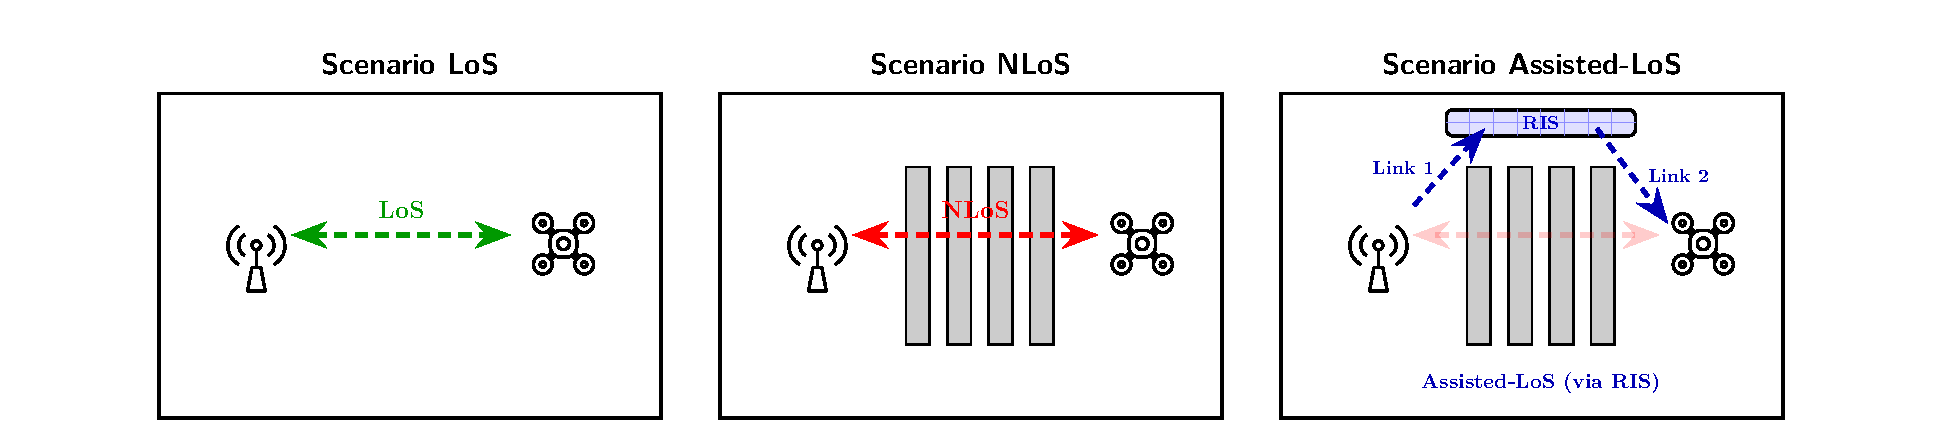
\includegraphics[width=0.95\textwidth]{../los_nlos_schema.pdf}
    \caption{Confronto schematico tra condizione di visibilità diretta (LoS) e ostruzione totale (NLoS) in ambiente industriale magazzino.}
    \label{fig:los_nlos_comparison}
\end{figure}





\clearpage
\subsection{Motivazione: Limiti NLoS industriali e necessità di architetture 6G-ready}

Le future reti di sesta generazione (6G) si pongono l'obiettivo di abilitare una connettività ubiqua e ultra-veloce sfruttando porzioni di spettro ad oggi poco esplorate, come le bande millimetriche (mmWave) e il terahertz (THz). Tuttavia, l'integrazione di tali segnali in ambienti industriali complessi è ostacolata da severi limiti fisici: le onde ad alta frequenza presentano capacità di penetrazione pressoché nulle e sono estremamente vulnerabili al blocco causato da ostacoli fisici. In contesti logistici, la presenza di imponenti infrastrutture metalliche e scaffalature ad alta densità (corridoi VNA) ostruisce sistematicamente i percorsi in visibilità diretta (Line-of-Sight, LoS), confinando la comunicazione in un regime di Non-Line-of-Sight (NLoS) \cite{Gebretsadik2024,Poddar2024}. Mentre le tecnologie tradizionali Multiple-Input Multiple-Output (MIMO) operano efficacemente per mitigare il fading su piccola scala, esse risultano strutturalmente insufficienti nel contrastare il fading su larga scala (shadowing) indotto dalle ostruzioni fisiche totali.

Per superare questo stallo propagativo, la ricerca si è focalizzata sulle Reconfigurable Intelligent Surfaces (RIS). Tali superfici, composte da elementi riflettenti a basso costo, permettono di direzionare il fascio elettromagnetico verso zone d'ombra altrimenti isolate. Tuttavia, le RIS puramente passive soffrono di un limite sistemistico fondamentale: l'effetto di fading moltiplicativo \cite{Zhang2022}. In un collegamento assistito da RIS passiva, il path loss equivalente del canale a cascata è proporzionale al prodotto (e non alla somma) delle attenuazioni dei singoli tratti (TX-RIS e RIS-RX). Questa degradazione quadratica rende i collegamenti riflessi estremamente deboli rispetto a un link diretto, rendendo necessario l'impiego di un numero inattuabile di elementi (migliaia di unit cells) per ottenere un guadagno di capacità apprezzabile in scenari NLoS.

Diviene quindi imperativo il passaggio verso architetture 6G-ready basate sull'impiego di RIS attive integrate su piattaforme mobili. A differenza dei modelli passivi, le RIS attive incorporano amplificatori a riflessione che consentono di compensare il fading moltiplicativo, pur introducendo un contributo di rumore termico dinamico che deve essere modellato con precisione \cite{Zhang2022,Wei2024}. In un ecosistema industriale dinamico, l'efficacia di tali superfici è ulteriormente potenziata dal loro montaggio a bordo di droni (UAV) \cite{Muller2024,Azizi2024}. L'integrazione UAV-RIS conferisce al sistema gradi di libertà spaziali senza precedenti: la capacità di riposizionamento in tempo reale permette di stabilire link in prossimità e in LoS sia verso la Base Station che verso il target, garantendo i requisiti di affidabilità e latenza (URLLC) necessari per le moderne operazioni di robotica autonoma.

\subsection{Obiettivi del Lavoro: Tracking sub-metrico, abbattimento dell'outage e ottimizzazione dell'efficienza energetica (Green 6G)}



L'obiettivo primario di questo lavoro di tesi è la progettazione, lo sviluppo e la simulazione di un'architettura di rete di sesta generazione (6G) in grado di garantire il tracciamento continuo e ad altissima precisione (sub-metrico o centimetrico) di droni (UAV) in ambienti industriali severamente ostruiti. Parallelamente, il sistema mira all'abbattimento radicale dell'outage di segnale e alla massimizzazione dell'efficienza energetica sistemistica, allineandosi ai paradigmi emergenti del "Green 6G".

Per quanto concerne il tracking sub-metrico, la sfida ingegneristica risiede nell'effettuare una localizzazione autonoma utilizzando ricevitori a singola antenna a bordo dell'UAV, scartando i tradizionali (e ingombranti) array di antenne per ragioni di efficienza energetica e di spazio \cite{Ye2023}. In assenza di segnale GNSS (Global Navigation Satellite System), il drone deve stimare la propria posizione unicamente tramite l'osservazione dei segnali radio riflessi dalle Reconfigurable Intelligent Surfaces (RIS). Il cuore algoritmico del tracciamento si basa sull'impiego del Filtro di Kalman Esteso (EKF). L'EKF è un filtro autoregressivo ottimizzato per sistemi dinamici non lineari: esso opera attraverso un ciclo iterativo di "predizione-correzione" in cui bilancia l'incertezza del modello di stato del drone (rumore di processo, velocità, fluttuazioni di orientamento) con l'incertezza delle osservazioni radio, minimizzando l'errore quadratico medio della stima \cite{Muller2024,Ye2023}. L'impiego congiunto dell'EKF e di setup a più RIS (multi-RIS deployment) permette di creare delle vere e proprie "impronte digitali" (fingerprint) radio estremamente distinguibili nell'ambiente, consentendo una convergenza rapida del filtro e un errore di posizionamento che scende al livello centimetrico \cite{Ye2023}.

Il secondo obiettivo cruciale è l'abbattimento dell'outage, inteso come la prevenzione della caduta del link radio e la massimizzazione del rapporto segnale-interferenza-più-rumore (SINR). L'uso di superfici riflettenti passive può generare un inquinamento spettrale, poiché le RIS non riescono nativamente a distinguere il segnale desiderato da eventuali segnali interferenti presenti nel medesimo ambiente \cite{Wang2024}. Per risolvere questo problema, il lavoro propone l'adozione di un controllo dinamico (ON-OFF) delle RIS guidato dalla predizione della traiettoria. Sfruttando reti neurali ricorrenti, come le Long Short-Term Memory (LSTM), la stazione base può inferire le coordinate future degli UAV. Sulla base di questa predizione spaziale, il sistema può pre-calcolare le configurazioni di fase ottimali e decidere dinamicamente quali RIS attivare o spegnere, mitigando proattivamente le interferenze di co-canale e l'outage \cite{Wang2024}.

Infine, il lavoro si pone l'obiettivo dell'ottimizzazione dell'efficienza energetica sistemistica (AEE - Absolute Energy Efficiency), quantificata in bit/Joule. In contesti di Logistica 4.0, l'impiego di hardware sostenibile è vitale. La tesi esplora l'adozione delle Beyond-Diagonal RIS (BD-RIS), un'evoluzione delle metasuperfici che permette una gestione più flessibile dello scattering e una riflettività superiore, riducendo la potenza emissiva necessaria alla Base Station \cite{Khan2024}. Per massimizzare l'efficienza senza violare i vincoli hardware, viene implementato l'algoritmo di Dinkelbach. Questo metodo matematico permette di risolvere il problema di ottimizzazione frazionaria dell'efficienza energetica, individuando il punto di operatività ottimo sul fronte di Pareto tra throughput di rete e consumo termodinamico \cite{Khan2024}. Poiché tali calcoli complessi richiedono risorse incompatibili con l'hardware di bordo, l'architettura delega l'intero onere computazionale al RAN Intelligent Controller (RIC) all'interno di un paradigma Open RAN (O-RAN), garantendo che l'intera flotta UAV operi con il massimo risparmio energetico possibile pur mantenendo un collegamento ininterrotto e ultra-preciso \cite{Lien2024}.

\subsection{Metodologia: Sviluppo del Digital Twin in Python e struttura dell'elaborato}

Per validare sperimentalmente i paradigmi teorici delle reti 6G assistite da RIS, il presente lavoro si fonda sulla progettazione e sullo sviluppo di un simulatore custom ad alte prestazioni implementato in linguaggio Python. Data l'impraticabilità economica e le limitazioni fisiche di un testbed reale su larga scala, si è optato per la creazione di un Digital Twin (Gemello Digitale). Questo ambiente di simulazione opera come un motore deterministico capace di replicare fedelmente la topologia tridimensionale di un magazzino logistico (discretizzando le scaffalature metalliche tramite volumi di delimitazione Axis-Aligned Bounding Boxes, AABB), la cinematica di volo degli UAV e le dinamiche di propagazione elettromagnetica a 5.9 GHz in regime di severo NLoS.

Dal punto di vista del software engineering, il simulatore adotta un'architettura che separa nettamente il Data Plane (il dominio fisico vettoriale) dal Control Plane (il Server Centrale SDN), emulando i ritardi di comunicazione tramite chiamate gRPC \cite{Vairam2023}. Per superare i colli di bottiglia computazionali intrinseci di Python -- in particolare il Global Interpreter Lock (GIL) -- l'architettura sfrutta il paradigma del Multiprocessing accoppiato a un gestore di Shared Memory a basso livello. Questa ingegnerizzazione permette ai moduli di scambiare i tensori di stato operando in logica Zero-Copy, garantendo latenze di interscambio nell'ordine dei nanosecondi. Inoltre, i calcoli intensivi per il Ray-Casting radio sono stati ottimizzati tramite alberi k-dimensionali (KDTree) per abbattere la complessità della ricerca a $\mathcal{O}(\log N)$, e tramite compilazione Just-In-Time (JIT) (libreria Numba) per accelerare le operazioni matriciali.

L'evoluzione dello stato è garantita da un Simulation Clock deterministico in cui il tempo $t_k$ avanza in modo discreto secondo l'equazione $t_k = k \cdot \Delta t$, con un passo $\Delta t = 0.1$ s. La metrica cardine per la valutazione delle prestazioni è l'Errore Quadratico Medio (RMSE) spaziale, calcolato come la norma euclidea tra le coordinate reali di volo e quelle stimate dal filtro EKF \cite{Muller2024,Ye2023}.

\subsubsection*{Struttura dell'elaborato}
La tesi è strutturata in sei capitoli come segue:
\begin{itemize}[leftmargin=2.8cm, labelwidth=2.5cm, labelsep=0.3cm, itemindent=0cm, align=left]
    \item[\textbf{Capitolo 1:}] Introduzione al contesto della Logistica 4.0, analisi dei limiti NLoS e presentazione della metodologia del Digital Twin.
    \item[\textbf{Capitolo 2:}] Esplora il Modello Fisico e la Propagazione Radio 6G, dettagliando il modello di canale 3GPP TR 38.901 per lo scenario InF-DH \cite{Gebretsadik2024,Poddar2024}, gli algoritmi di Ray-Casting per la validazione spaziale \cite{Huang2022} e il calcolo del Link Budget in cascata derivante dall'uso di RIS attive \cite{Zhang2022} e BD-RIS \cite{Khan2024}.
    \item[\textbf{Capitolo 3:}] Si concentra sull'Architettura di Rete e sui Protocolli SDN, analizzando la transizione verso la Service-Based Architecture (SBA) \cite{Kolakowski2024}, l'accesso Grant-Free nel livello MAC \cite{Yu2024}, l'ottimizzazione del livello di trasporto tramite gRPC \cite{Vairam2023} e il ruolo del Near-RT RIC in ottica O-RAN per la sicurezza a livello fisico \cite{Lien2024}.
    \item[\textbf{Capitolo 4:}] Scende nel dettaglio dell'ingegneria del software del simulatore Python, sviscerando il motore cinematico, la formulazione matematica dell'Extended Kalman Filter (EKF) \cite{Muller2024,Ye2023}, le logiche predittive (tramite reti LSTM) del controller SDN \cite{Wang2024,Wei2024} e le tecniche di ottimizzazione computazionale adottate per scalare il sistema.
    \item[\textbf{Capitolo 5:}] Corona il lavoro con la Validazione Sperimentale e l'Analisi dei Risultati, presentando i dati estratti dal simulatore in quattro scenari di test: Baseline NLoS (Test 1), Assisted-LoS (Test 2), Stress Test Latenza \cite{Vairam2023,Lien2024} (Test 3) e Controllo Predittivo orientato all'efficienza energetica \cite{Wang2024,Khan2024} (Test 4).
    \item[\textbf{Capitolo 6:}] Riassume le conclusioni del lavoro e delinea i possibili sviluppi futuri della ricerca.
\end{itemize}

\clearpage
\section{Modello Fisico e Propagazione Radio 6G}
\subsection{Il Canale 3GPP TR 38.901: Modellazione InF-DH a 5.9 GHz}

Lo sviluppo di un Digital Twin affidabile per il tracciamento di UAV in ambito industriale richiede una modellazione rigorosa e standardizzata del mezzo radiopropagativo. Nelle reti cellulari di sesta generazione (6G), lo spettro delle frequenze Sub-6 GHz (e in particolare la banda attorno ai 5.9 GHz) assume un ruolo strategico: esso offre un compromesso ottimale tra capacità di trasmissione dati e resilienza alla propagazione rispetto alle più sensibili frequenze millimetriche (mmWave) \cite{Gebretsadik2024,Poddar2024}. Per simulare matematicamente le dinamiche di attenuazione del segnale in un magazzino logistico, il presente lavoro adotta il modello di canale ufficiale 3GPP TR 38.901, validato per frequenze operative comprese tra 0.5 e 100 GHz \cite{Poddar2024}.

All'interno di questo standard, lo scenario specifico che meglio approssima la topologia di un ambiente VNA (Very Narrow Aisle) è identificato come InF-DH (Indoor Factory with Dense Clutter and High Base Station). In questo scenario, le Stazioni Radio Base (BS) sono posizionate in elevazione rispetto al clutter circostante (le scaffalature metalliche). Tuttavia, l'elevata densità degli ostacoli sottostanti genera un ambiente di propagazione severo, dominato da complessi fenomeni di scattering e forti attenuazioni da penetrazione.

Il modello 3GPP calcola la perdita di percorso totale (Path Loss, PL) in scenari Indoor Hotspot (InH) e industriali sommando diverse componenti fisiche. Nei casi in cui è garantita una visibilità diretta (Line-of-Sight, LoS) tra il trasmettitore e l'UAV, l'attenuazione dipende primariamente dalla Free Space Path Loss (FSPL), la quale scala logaritmicamente in funzione della distanza tridimensionale ($d_{3D}$) e della frequenza della portante ($f_c$). Secondo le specifiche 3GPP TR 38.901 per scenari InH in visibilità diretta, la formula generale del Path Loss (espresso in dB) è definita come segue \cite{Poddar2024}:

% Equazione 2.1: Path Loss in Line-of-Sight (LoS)
\begin{equation} 
PL_{LOS} = 32.4 + 17.3 \log_{10}(d_{3D}) + 20 \log_{10}(f_c) + \mathcal{N}(0, \sigma_{SF}^2) \label{eq:pl_los} 
\end{equation} 

A questa componente deterministica si aggiunge lo Shadow Fading, modellato tramite l'estrazione da una variabile aleatoria gaussiana $\mathcal{N}(0, \sigma_{SF}^2)$ a media nulla e varianza $\sigma_{SF}^2$. Questo termine stocastico modella le fluttuazioni a lenta variazione (macroscopiche) del segnale causate dall'ombreggiamento degli ostacoli circostanti \cite{Poddar2024}.

Tuttavia, all'interno dei corridoi metallici InF-DH, l'UAV opera prevalentemente in condizioni di Non-Line-of-Sight (NLoS). In questo regime, il segnale elettromagnetico che attraversa le fitte scaffalature in acciaio subisce una drastica Penetration Loss (attenuazione per penetrazione). Nel modello matematico implementato all'interno del simulatore (Digital Twin), tale attenuazione supplementare è calcolata dinamicamente in modo proporzionale alla profondità geometrica ($d_{metal}$) del volume metallico attraversato dal raggio radio. In ambienti industriali pesanti, questo fattore decurta il segnale di svariati decibel per ogni metro di compenetrazione.

Nel contesto specifico del layout InF-DH simulato, l'equazione ibrida (deterministica-stocastica) che computa il Path Loss totale in presenza di blocco NLoS indotto dal clutter metallico è implementata come segue:

% Equazione 2.2: Path Loss Totale in Non-Line-of-Sight (NLoS) con ostruzione metallica 
\begin{equation} 
PL_{tot}(d) = 31.84 + 21.50 \log_{10}(d_{3D}) + 19 \log_{10}(f_c) + \mathcal{N}(0, \sigma_{SF}^2) + (\gamma_{pen} \cdot d_{metal}) \label{eq:pl_nlos_metal} 
\end{equation}

\clearpage
Dove:
\begin{itemize}
    \item $f_c$ è la frequenza centrale operativa espressa in GHz (nel nostro caso 5.9 GHz).
    \item $d_{3D}$ è la distanza tridimensionale tra trasmettitore e ricevitore in metri.
    \item $\sigma_{SF}$ è la deviazione standard dello Shadowing (impostata a 3.5 dB per lo scenario in esame).
    \item $\gamma_{pen}$ rappresenta il coefficiente di attenuazione per penetrazione del materiale (es. 15 dB/m per l'acciaio strutturale).
    \item $d_{metal}$ è lo spessore dell'ostacolo effettivamente attraversato, misurato in metri tramite algoritmi geometrici vettoriali.
\end{itemize}

Questa rigorosa formulazione matematica permette al motore di propagazione di restituire valori realistici e tempo-varianti del rapporto segnale-rumore (SNR) e dell'indicatore di potenza del segnale ricevuto (RSSI), parametri che costituiscono l'input vitale per il successivo stadio di elaborazione inerziale tramite filtro EKF.
\subsection{Validazione Spaziale NLoS: Algoritmi di Ray-Casting e attenuazione}

Nelle reti 6G operanti a frequenze Sub-6 GHz (come la banda a 5.9 GHz) e millimetriche, le onde elettromagnetiche sono estremamente suscettibili ai blocchi fisici \cite{Huang2022}. Per modellare accuratamente gli effetti di propagazione in ambienti indoor complessi, i modelli puramente stocastici tradizionali risultano insufficienti; si rende perciò necessario l'impiego di modelli deterministici basati sul Ray Tracing (tracciamento dei raggi), capaci di mappare esattamente l'interazione tra i raggi radio e la geometria dell'ambiente per determinare i percorsi di riflessione, diffrazione e trasmissione \cite{Huang2022}.

Nel Digital Twin sviluppato per questa tesi, la validazione spaziale del canale radio -- ovvero la determinazione esatta dello stato di Line-of-Sight (LoS) o Non-Line-of-Sight (NLoS) -- è affidata a un motore di Ray-Casting vettorializzato ad alte prestazioni. L'algoritmo non si limita a un controllo binario della visibilità, ma calcola analiticamente la profondità di penetrazione del segnale attraverso il clutter logistico. L'ambiente industriale è discretizzato modellando le scaffalature metalliche come volumi solidi di tipo AABB (Axis-Aligned Bounding Box). Ad ogni intervallo di simulazione temporale ($\Delta t$), l'algoritmo traccia un segmento vettoriale ideale che connette il trasmettitore (la Base Station o una RIS attiva) all'antenna ricevente a bordo dell'UAV in movimento.

Attraverso rigorose operazioni di calcolo vettoriale, il sistema valuta le intersezioni del raggio con i piani limitanti minimi e massimi degli ostacoli lungo gli assi tridimensionali X, Y e Z. Se l'algoritmo rileva che il raggio attraversa il volume della scatola di delimitazione, calcola in modo esatto i metri cumulativi di spessore metallico intersecati, denotati come $d_{metal}$. Questo parametro spaziale è vitale per l'accuratezza del Link Budget. In condizioni di NLoS, al Path Loss in spazio libero (FSPL) viene sommata un'attenuazione massiccia proporzionale allo spessore attraversato, quantificata dal modello in 15.0 dB per ogni metro di metallo penetrato. Questa severa degradazione deterministica abbatte drasticamente il rapporto segnale-rumore (SNR) al di sotto della soglia di sensibilità del ricevitore, innescando l'outage del collegamento radio e rendendo imperativo l'intervento delle RIS.

Dal punto di vista computazionale e dell'ingegneria del software, iterare il calcolo geometrico delle intersezioni su migliaia di volumi metallici per ogni drone rappresenterebbe un collo di bottiglia critico. I linguaggi ad alto livello soffrono dei limiti imposti dal Global Interpreter Lock (GIL), che impedisce un reale parallelismo. Per garantire la scalabilità del tracciamento in tempo reale, l'algoritmo di Ray-Casting è stato fortemente ottimizzato mediante la compilazione Just-In-Time (JIT). Tramite l'impiego di librerie LLVM (come Numba in ambiente Python), le funzioni spaziali vengono tradotte preventivamente in codice macchina, operando a velocità paragonabili ai linguaggi di basso livello e svincolandosi totalmente dal GIL (come dettagliato nel Capitolo 4). A questo si aggiunge l'impiego di alberi k-dimensionali (KDTree) per il partizionamento dello spazio, che riduce la complessità asintotica della ricerca delle collisioni a $\mathcal{O}(\log N)$, garantendo la tenuta del sistema anche in layout massivi VNA da decine di migliaia di metri quadrati.

Per la validazione spaziale, si modella l'equazione parametrica del raggio radio e si calcola l'attenuazione da penetrazione totale in base alle intersezioni AABB. L'equazione parametrica del raggio radio (per $t \in [0, L]$) è definita come:

% Equazione 2.3: Equazione parametrica del raggio radio
\begin{equation}
\vec{r}(t) = \mathbf{p}_{tx} + t \cdot \vec{d}_{dir} \quad \text{con} \quad \vec{d}_{dir} = \frac{\mathbf{p}_{rx} - \mathbf{p}_{tx}}{\|\mathbf{p}_{rx} - \mathbf{p}_{tx}\|_2} \label{eq:ray_parametric}
\end{equation}

Il calcolo della Penetrazione Loss totale ($PL_{pen\_tot}$) per gli $N_{box}$ ostacoli intersecati è dato da:

% Equazione 2.4: Calcolo della Penetration Loss da intersezioni AABB
\begin{equation}
PL_{pen\_tot} = PL_{pen} \cdot d_{metal} = PL_{pen} \cdot \sum_{i=1}^{N_{box}} \Big( \max\big(0, \min(\|\mathbf{p}_{rx}-\mathbf{p}_{tx}\|_2, t_{max,i})\big) - \max\big(0, t_{min,i}\big) \Big) \label{eq:pl_pen_tot}
\end{equation}

Dove $PL_{pen}$ è il fattore di attenuazione (es. 15 dB/m), mentre $t_{min,i}$ e $t_{max,i}$ rappresentano i parametri del raggio nei punti di entrata e di uscita dall'ostacolo $i$-esimo.
\subsection{Reconfigurable Intelligent Surfaces (RIS)}

L'introduzione delle Reconfigurable Intelligent Surfaces (RIS) rappresenta un salto paradigmatico per le reti 6G, abilitando per la prima volta la possibilità di ingegnerizzare attivamente l'ambiente radiopropagativo, trasformandolo da un'entità stocastica e ostile a un parametro di progetto ottimizzabile. Una RIS è una metasuperficie planare composta da un elevato numero di elementi riflettenti a basso costo (unit cells), ciascuno capace di alterare dinamicamente la fase e, in configurazioni avanzate, l'ampiezza dell'onda elettromagnetica incidente. Tale capacità permette di focalizzare l'energia del segnale verso un ricevitore target (beamforming riflesso), bypassando ostruzioni fisiche e instaurando un collegamento virtuale in visibilità (Assisted-LoS) \cite{Zhang2022}.

\begin{center}
    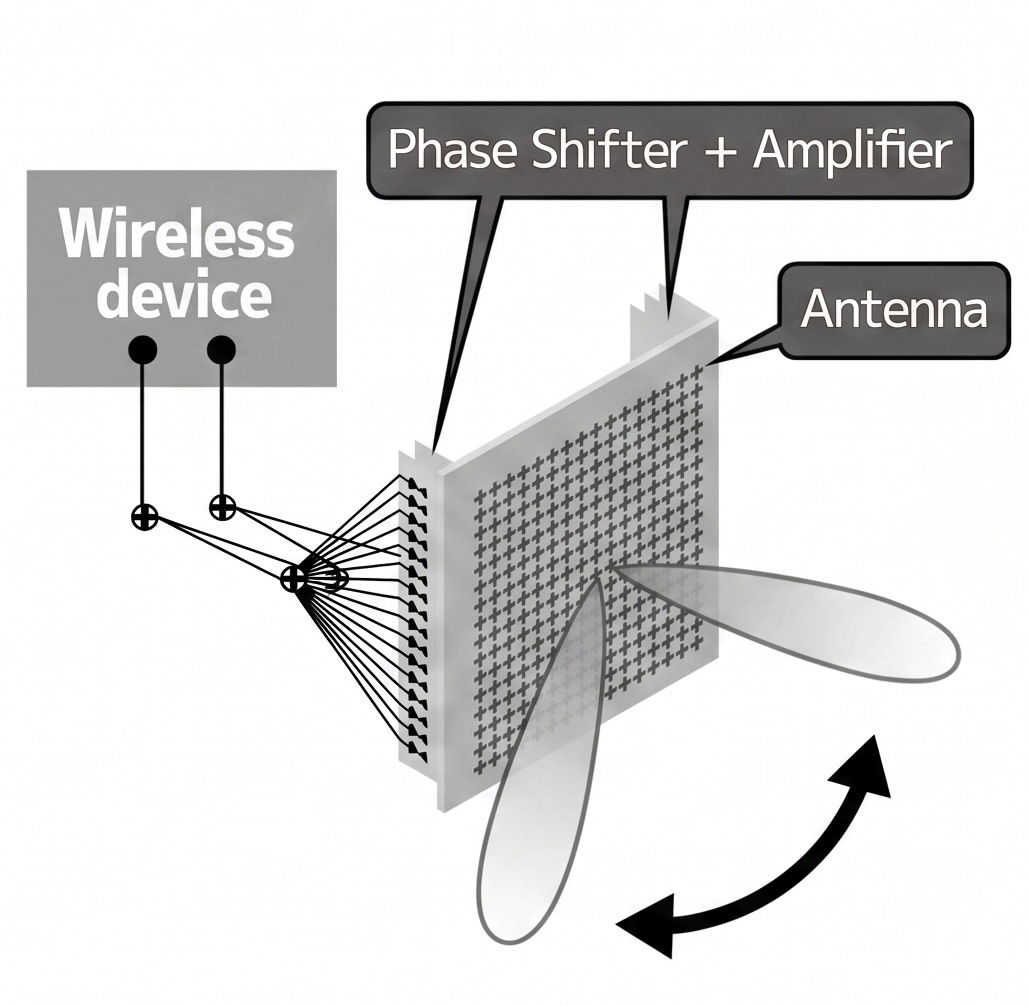
\includegraphics[width=0.3\textwidth]{Images/RIS.jpeg}
    \captionof{figure}{Rappresentazione concettuale di una RIS.}
    \label{fig:ris_concept}
\end{center}

\clearpage
\subsubsection{Il limite del Fading Moltiplicativo nelle RIS Passive}

Nella fase iniziale della ricerca, l'attenzione si è focalizzata sulle RIS puramente passive. Questi dispositivi utilizzano circuiti a impedenza variabile unicamente per il controllo di fase, offrendo un consumo energetico quasi nullo e l'assenza di rumore termico aggiuntivo \cite{Zhang2022}. Tuttavia, le RIS passive soffrono di una limitazione fisica fondamentale nota come multiplicative fading (fading moltiplicativo). In un sistema assistito da RIS passiva, l'attenuazione totale del canale a cascata (BS $\rightarrow$ RIS $\rightarrow$ UAV) è pari al prodotto delle attenuazioni delle singole tratte \cite{Zhang2022,Muller2024}.

Matematicamente, il modello di ricezione per un canale a cascata tramite RIS passiva con $M$ elementi è definito come:

% Equazione 2.5: Canale efficace tramite RIS Passiva (Multiplicative Fading) 
\begin{equation} 
h_{eff} = \sum_{m=1}^{M} h_m A_m e^{j\varphi_m} g_m 
\label{eq:ris_passive_model} 
\end{equation} 

Dove $h_m$ e $g_m$ sono le risposte impulsive dei canali BS-RIS e RIS-UAV, mentre $A_m e^{j\varphi_m}$ rappresenta il coefficiente di riflessione dell'$m$-esimo elemento (con ampiezza vincolata a $A_m \leq 1$). Nei severi ambienti industriali indoor, questo effetto moltiplicativo rende il segnale riflesso estremamente debole, richiedendo array con decine di migliaia di elementi per eguagliare il guadagno di un link LoS standard, un requisito spaziale e computazionale spesso proibitivo per installazioni agili \cite{Zhang2022}.


\subsubsection{Architettura delle RIS Attive e gestione "Green 6G"}

Per superare il collo di bottiglia del fading moltiplicativo, l'architettura proposta in questo lavoro adotta il paradigma delle RIS attive. A differenza dei modelli passivi, ogni elemento di una RIS attiva integra un micro-amplificatore a radiofrequenza a riflessione (reflection-type amplifier) \cite{Zhang2022}. Questo componente non solo regola lo sfasamento, ma amplifica attivamente l'onda riflessa, compensando la severa attenuazione di percorso. Nel Digital Twin sviluppato, operante a 5.9 GHz, l'hardware è modellato come una matrice di 16$\times$16 elementi ($M=256$) con un guadagno attivo nominale di +20.0 dB.

Il segnale riflesso da una RIS attiva è modellato dalla seguente equazione:

% Equazione 2.6: Segnale riflesso da RIS Attiva (con Noise Figure) 
\begin{equation} 
\mathbf{y} = \mathbf{\Psi}\mathbf{x} + \mathbf{\Psi}\mathbf{v} + \mathbf{n}_s 
\label{eq:ris_active_signal} 
\end{equation} 

Dove $\mathbf{\Psi} = \text{diag}(p_1 e^{j\theta_1},\dots,p_N e^{j\theta_N})$ è la matrice di riflessione attiva (con guadagno $p_n > 1$), $\mathbf{x}$ è il segnale incidente, $\mathbf{\Psi}\mathbf{v}$ rappresenta il rumore dinamico introdotto e amplificato dai componenti attivi (modellato con una Noise Figure di 3.0 dB), e $\mathbf{n}_s$ è il rumore statico dell'hardware \cite{Zhang2022}. Per bilanciare le prestazioni con la sostenibilità energetica (Green 6G), il controller SDN gestisce la RIS in due stati: una modalità Active (consumo $\approx 50$ W) attivata solo quando l'SNR scende sotto la soglia critica di 5 dB, e una modalità Sleep (consumo 0.5 W) in cui gli amplificatori vengono disalimentati \cite{Wang2024}. 

\begin{figure}[H]
    \centering
    \begin{subfigure}[b]{0.48\textwidth}
        \centering
        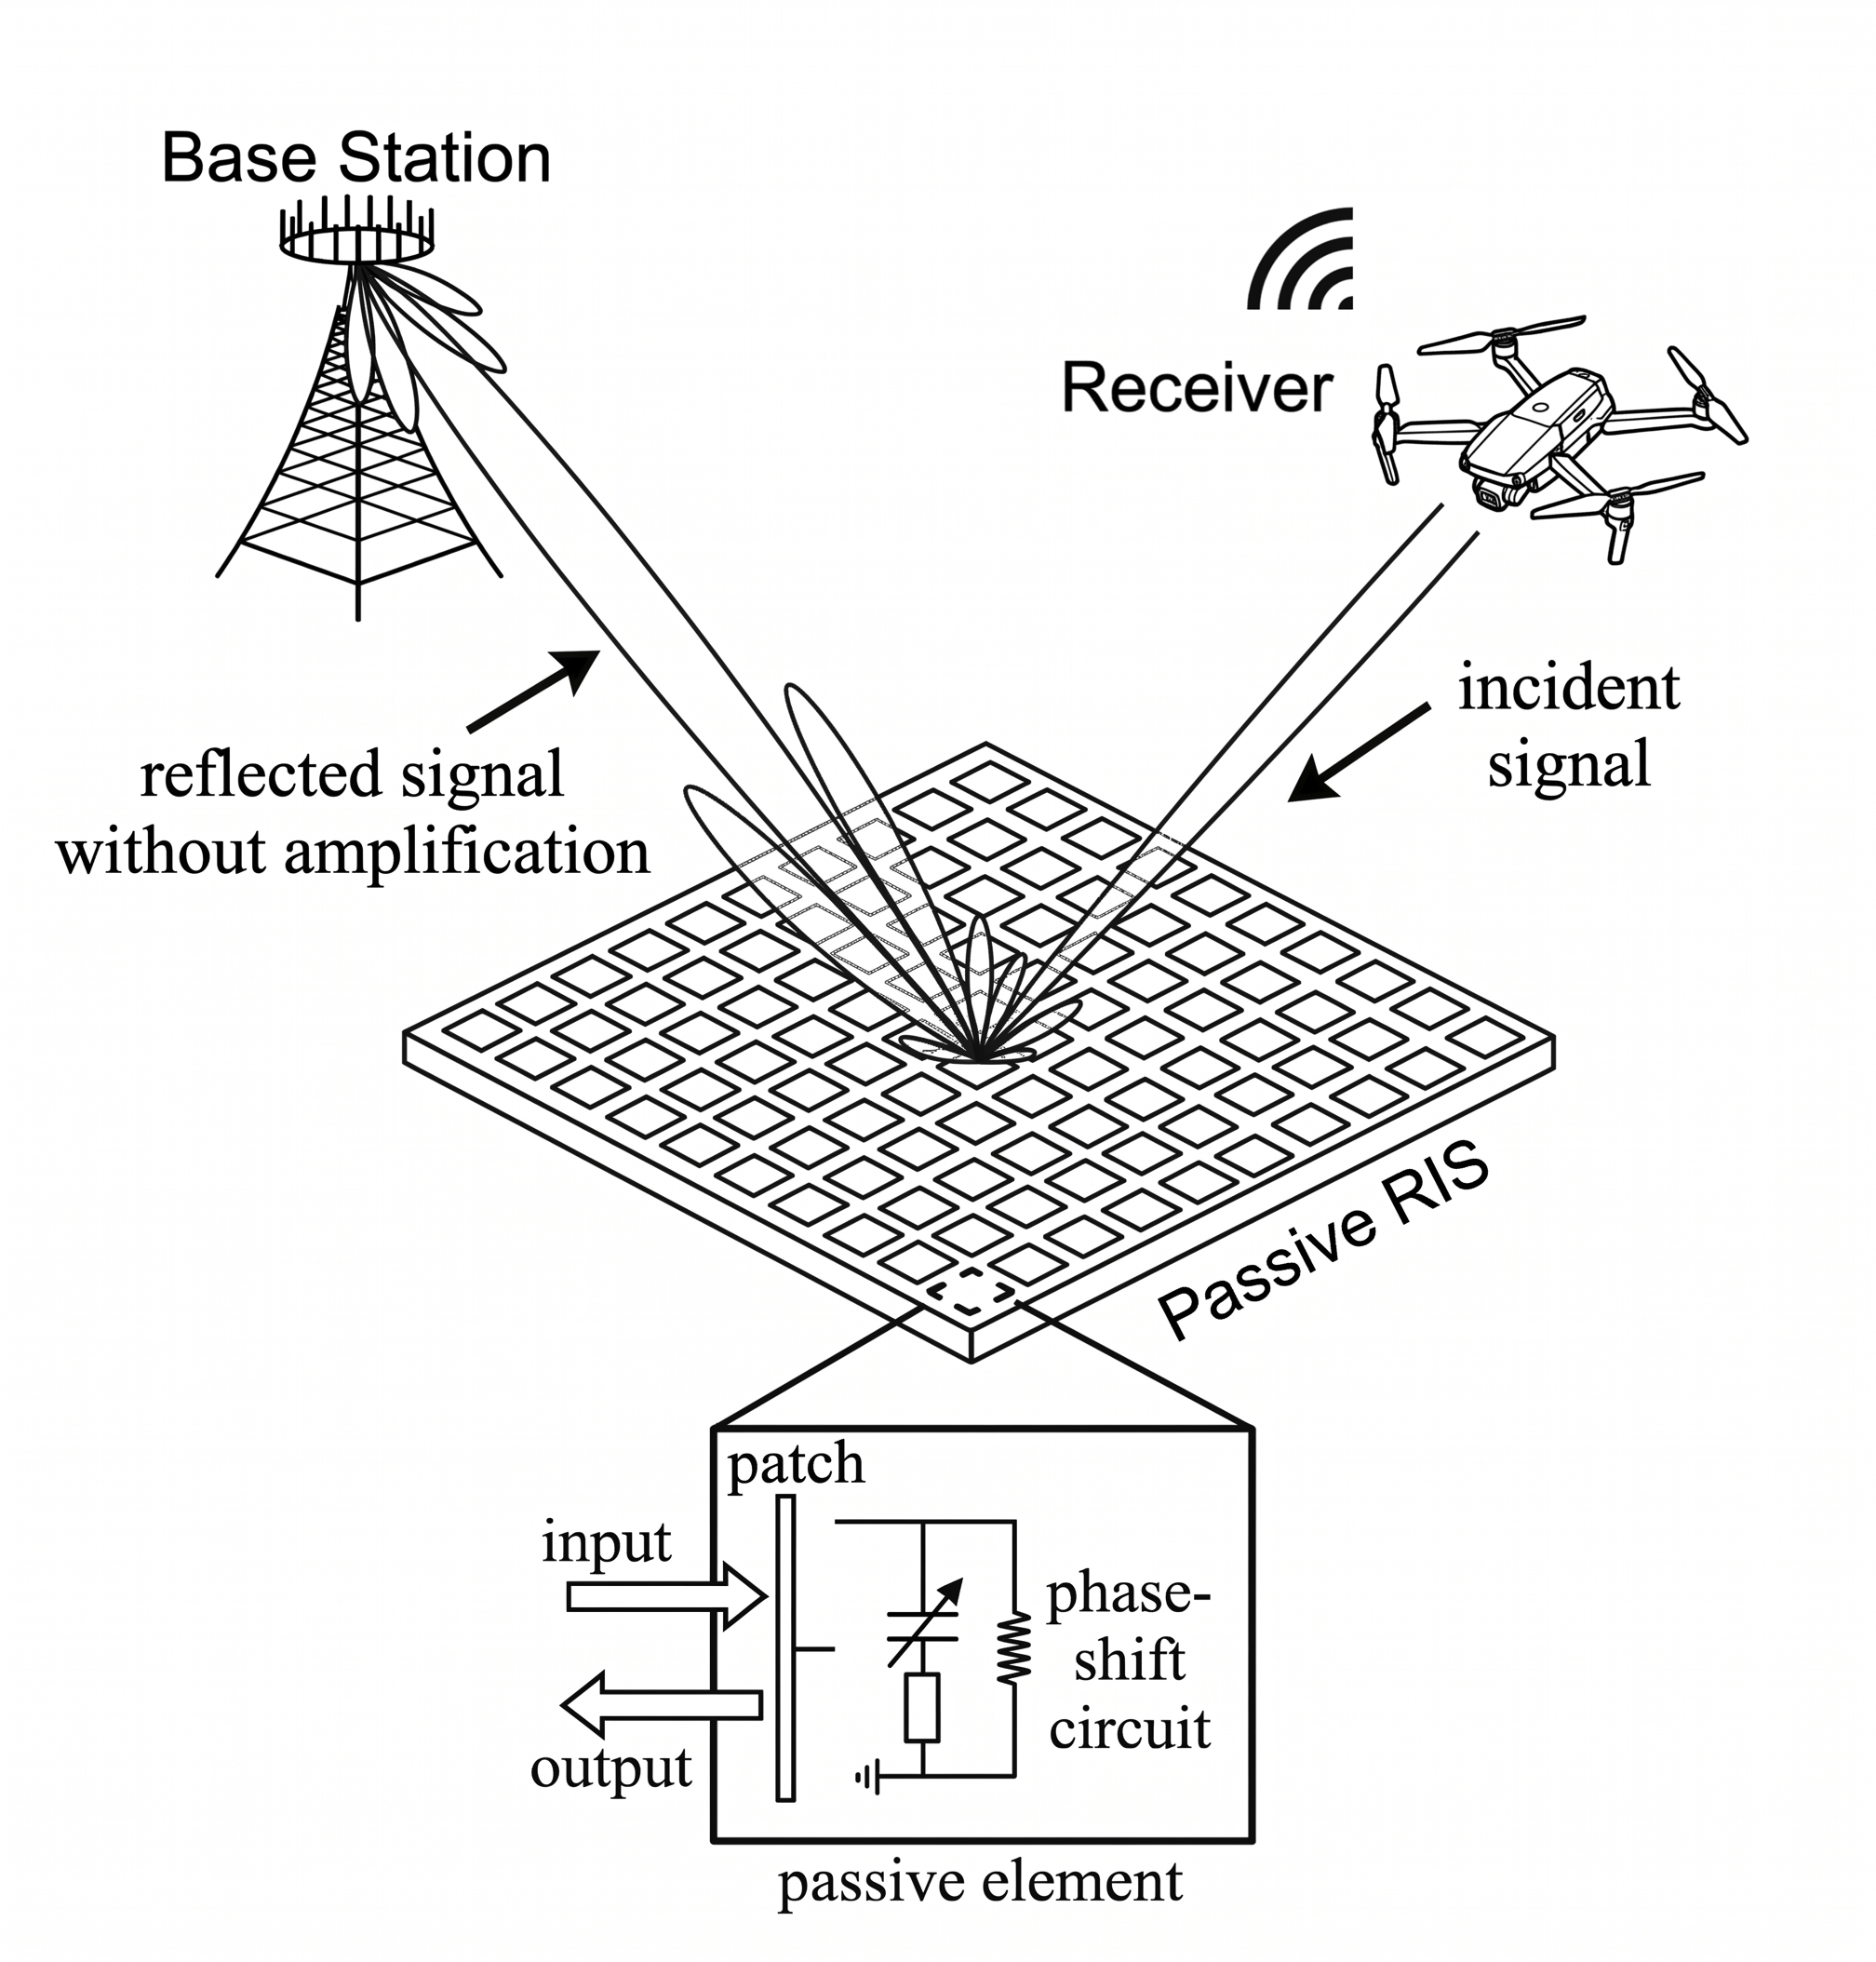
\includegraphics[width=\textwidth]{Images/ris_passiva_1.png}
        \caption{Passive RIS (Fading Moltiplicativo)}
        \label{fig:passive_ris}
    \end{subfigure}
    \hfill
    \begin{subfigure}[b]{0.48\textwidth}
        \centering
        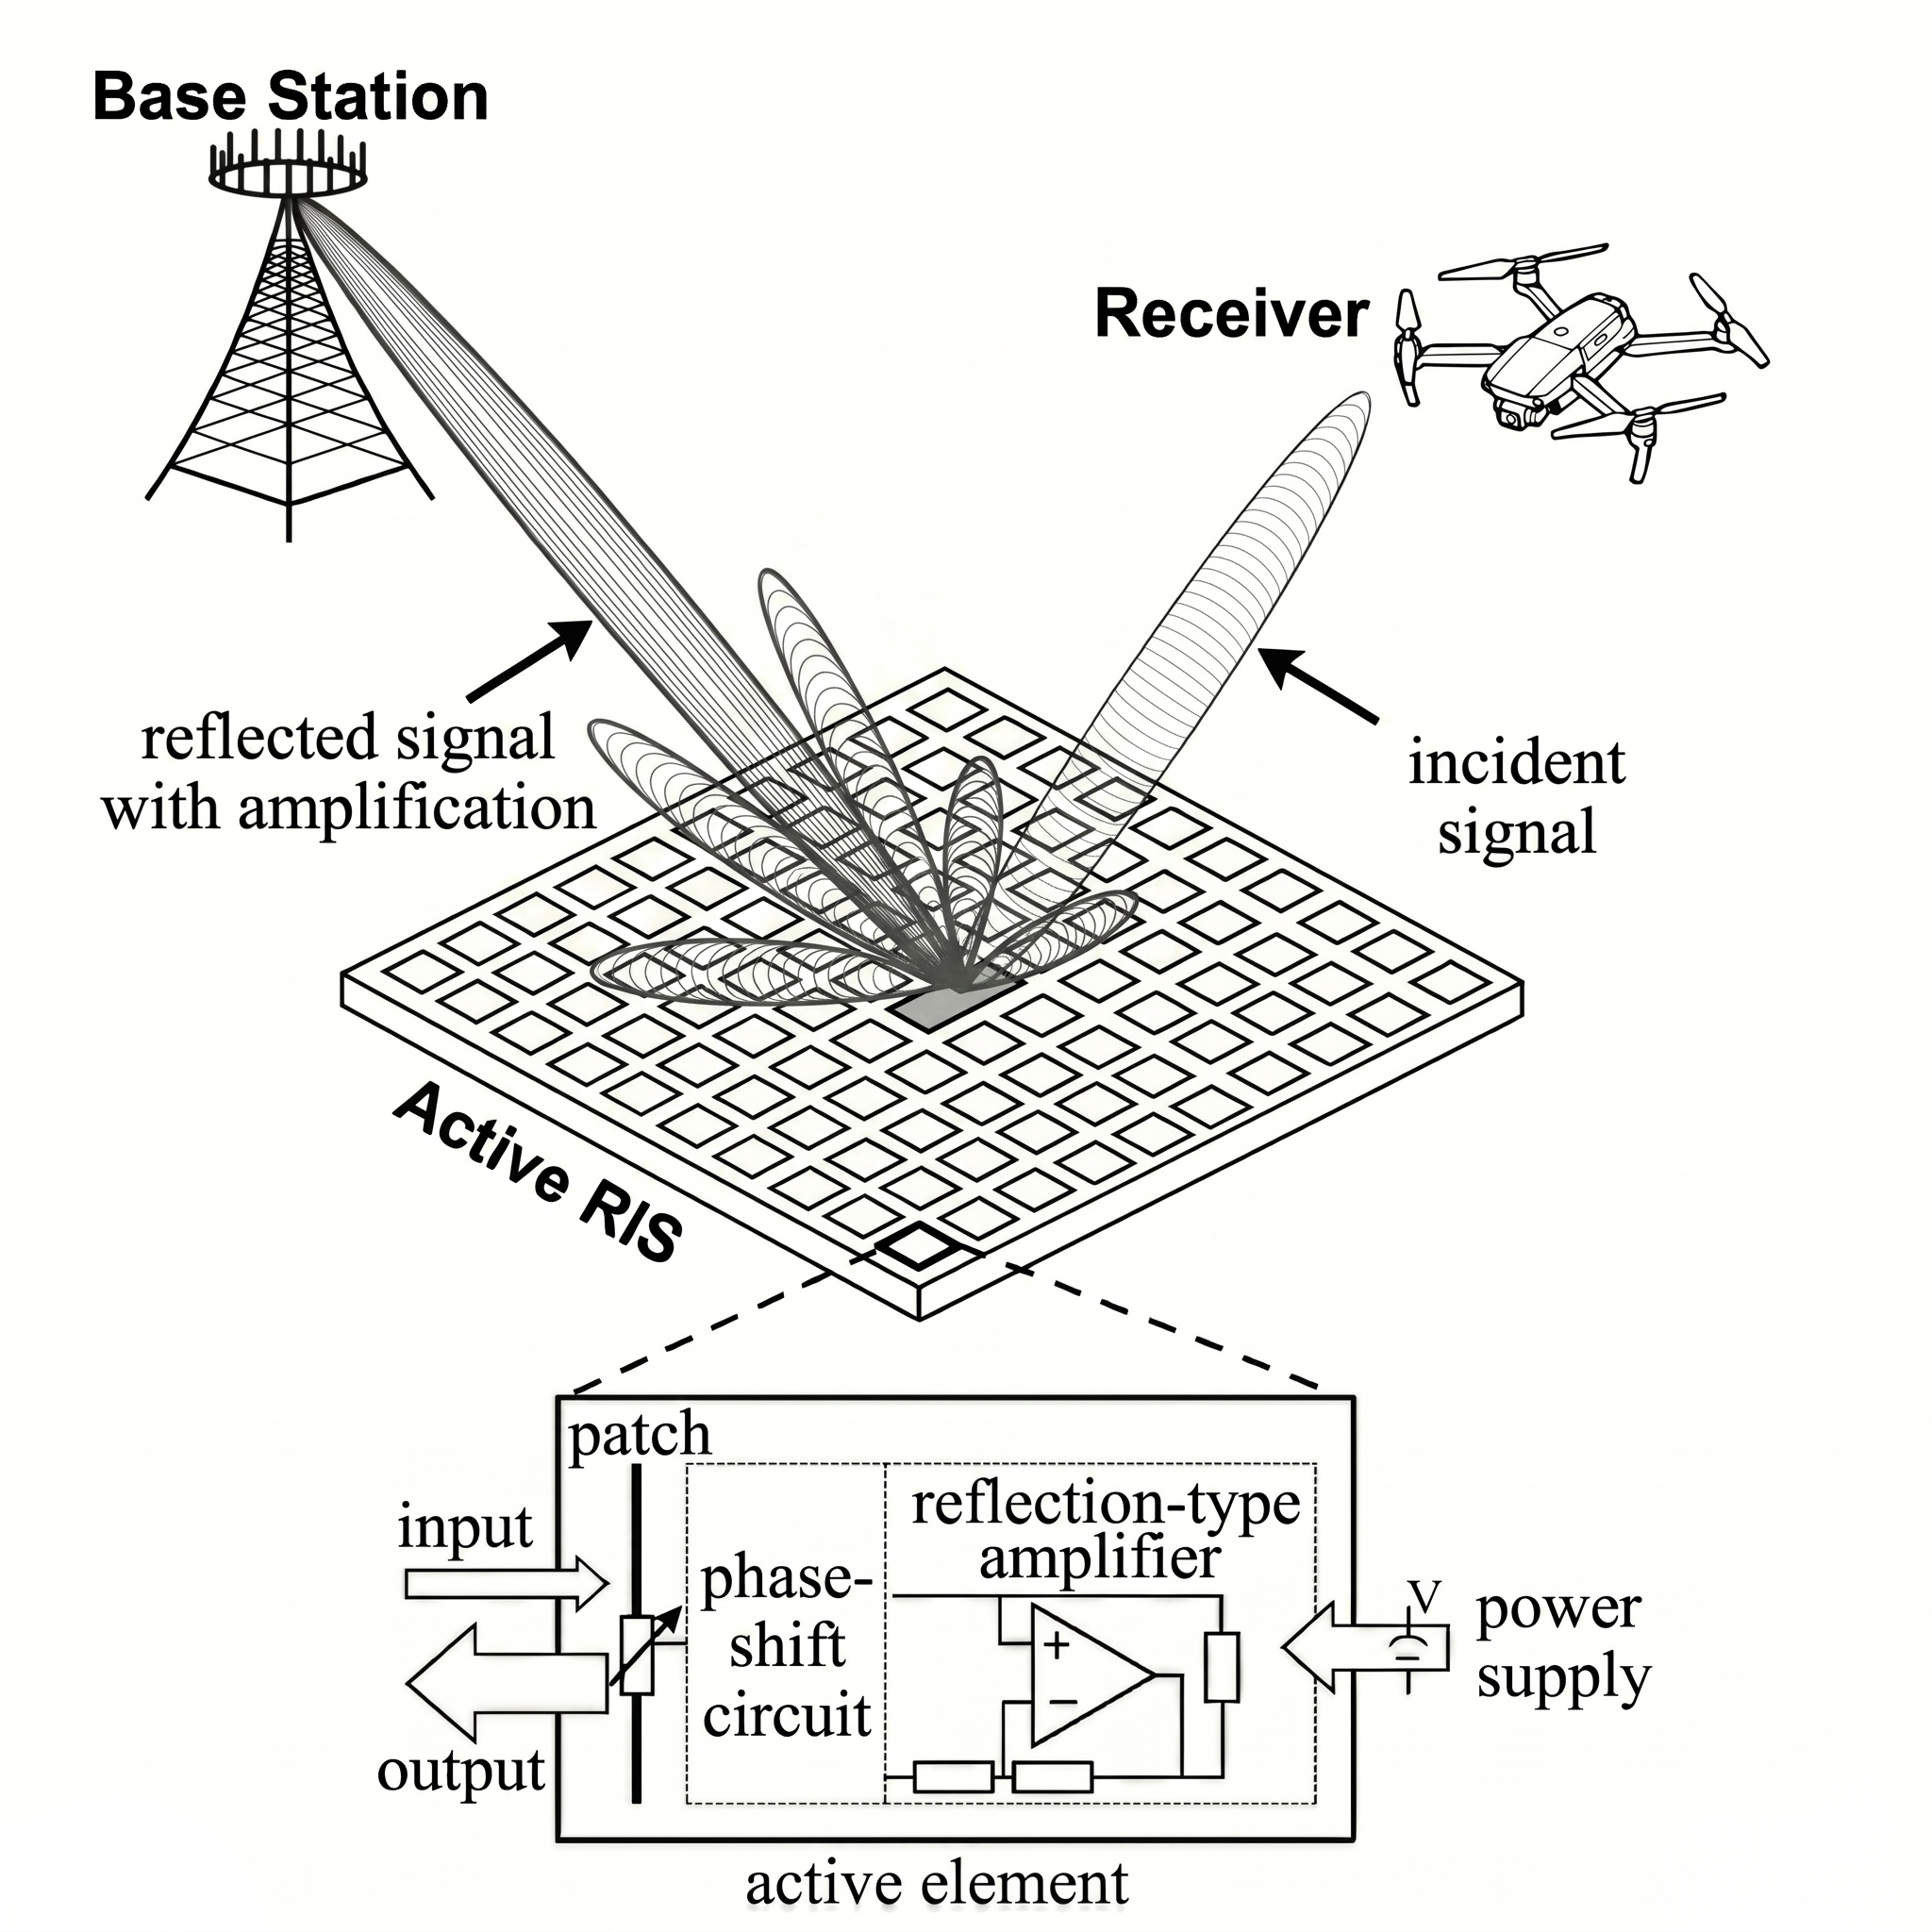
\includegraphics[width=\textwidth]{Images/ris_attiva_1.png}
        \caption{Active RIS (Amplificazione a Riflessione)}
        \label{fig:active_ris}
    \end{subfigure}
    \caption{Confronto architettonico tra Reconfigurable Intelligent Surfaces. (a) La propagazione passiva limitata dall'attenuazione moltiplicativa. (b) L'architettura attiva con micro-amplificatori per la mitigazione del path loss.}
    \label{fig:ris_comparison}
\end{figure}

\subsubsection{Transizione verso le Beyond-Diagonal RIS (BD-RIS)}

Il traguardo finale della ricerca, propedeutico all'ottimizzazione energetica del Test 4, è l'impiego delle Beyond-Diagonal RIS (BD-RIS). Mentre le RIS tradizionali sono limitate da matrici di scattering diagonali (dove ogni elemento riflette il segnale indipendentemente), le BD-RIS introducono interconnessioni circuitali tra gli elementi riflettenti \cite{Khan2024,Wei2024}. Questa architettura "oltre la diagonale" permette una flessibilità senza precedenti nella manipolazione dei fronti d'onda, migliorando l'efficienza energetica assoluta (AEE) e la soppressione delle interferenze di co-canale. L'ottimizzazione di tali superfici richiede algoritmi complessi come il metodo di Dinkelbach per risolvere problemi di programmazione frazionaria non convessi, massimizzando il rapporto bit/Joule dell'intero sistema \cite{Khan2024}.

\subsubsection{Imperfezioni Hardware e Beam Misalignment}

In scenari UAV, il sistema deve infine confrontarsi con il Beam Misalignment (disallineamento del fascio) causato dalla cinematica del drone. Data l'estrema direttività dei fasci a frequenze 6G, le fluttuazioni di assetto del drone (rollio/beccheggio) degradano la qualità del link \cite{Muller2024}. Il Digital Twin implementa una penalizzazione lineare che simula la perdita di collegamento RF quando l'errore angolare $\theta_{error}$ supera la tolleranza di $5^\circ$: 

% Equazione 2.7: Beam Misalignment Loss (Penalizzazione Assetto UAV) 
\begin{equation} 
L_{mis} = \max\left(0, \min\left(15.0, (\theta_{error} - 5^\circ) \cdot 0.5\right)\right) 
\label{eq:beam_misalignment} 
\end{equation}

Questa modellazione garantisce che la validazione sperimentale non sia basata su assunzioni ideali, ma rifletta le reali sfide di un deployment robotico industriale.
\subsection{Link Budget in Cascata nel canale UAV-RIS-BS}

Il calcolo del Link Budget in cascata costituisce un passaggio fondamentale per quantificare le prestazioni del canale radio (UAV-RIS-BS) quando il collegamento diretto in ambiente industriale è severamente ostruito. A differenza delle RIS passive, le quali subiscono l'effetto del fading moltiplicativo e si limitano a riflettere l'onda incidente perdendo drasticamente potenza, l'architettura a RIS attive impiegata in questo lavoro amplifica il segnale per compensare le perdite spaziali \cite{Zhang2022}. Tuttavia, l'uso di amplificatori a riflessione introduce una componente di rumore termico dinamico aggiuntiva che deve essere rigorosamente modellata nel bilancio di collegamento.

In un canale assistito da RIS attiva, il segnale ricevuto $\mathbf{y}$ alla Base Station (o all'UAV in fase di downlink) è descritto analiticamente dalla seguente equazione vettoriale \cite{Zhang2022}:

% Equazione 2.8: Segnale ricevuto con RIS Attiva (incluso rumore dinamico)
\begin{equation}
\mathbf{y} = \mathbf{h}_{r}^H \mathbf{\Psi} \mathbf{h}_{t} x + \mathbf{h}_{r}^H \mathbf{\Psi} \mathbf{v} + \mathbf{n}_s
\label{eq:active_ris_signal}
\end{equation}

Dove $\mathbf{h}_{t}$ e $\mathbf{h}_{r}$ sono i vettori di canale per le tratte trasmettitore-RIS e RIS-ricevitore, $x$ è il segnale utile trasmesso, e $\mathbf{\Psi}$ è la matrice diagonale di riflessione attiva. La criticità di questa formulazione risiede nei termini di rumore. Oltre al classico rumore termico statico del ricevitore $\mathbf{n}_s$ (il noise floor, modellato nel simulatore a $-90.0$ dBm), compare il termine $\mathbf{h}_{r}^H \mathbf{\Psi} \mathbf{v}$. Questo fattore modella il rumore dinamico $\mathbf{v}$ introdotto spontaneamente dalla circuiteria attiva della RIS, il quale viene a sua volta amplificato dalla matrice di guadagno $\mathbf{\Psi}$ e attenuato dal canale di propagazione $\mathbf{h}_{r}$ prima di giungere a destinazione \cite{Zhang2022}.

Analizzando il fenomeno nel dominio della potenza, il rumore dinamico amplificato scala in modo proporzionale alla norma di Frobenius della matrice di riflessione:

% Equazione 2.9: Potenza del rumore dinamico amplificato (Norma di Frobenius)
\begin{equation}
P_{noise\_dyn} \propto \|\mathbf{\Psi}\|_F^2 \sigma_v^2
\label{eq:dynamic_noise_power}
\end{equation}

Dove $\sigma_v^2$ è la varianza del rumore termico interno ai diodi attivi \cite{Zhang2022}. Nel Digital Twin sviluppato, questa complessa dinamica fisica viene sintetizzata in un calcolo deterministico del Signal-to-Noise Ratio (SNR) espresso in decibel. Assumendo una potenza di trasmissione dell'UAV ($P_{TX}$) pari a 20.0 dBm, l'energia irradiata subisce l'attenuazione totale per spazio libero e penetrazione degli ostacoli ($PL_{tot}$). L'attivazione della metasuperficie inietta nel sistema un guadagno di amplificazione nominale ($G_{RIS}$) di +20.0 dB, dal quale è tuttavia imperativo sottrarre la Noise Figure hardware ($NF_{RIS}$), stimata a 3.0 dB, per modellare l'inserimento del rumore dinamico sopracitato.

L'equazione algebrica del Link Budget computata dal Physics Engine del simulatore si esprime quindi come:

% Equazione 2.10: Calcolo dell'SNR logaritmico (Link Budget del Simulatore)
\begin{equation}
SNR_{dB} = P_{TX} - PL_{tot} - N_0 + G_{RIS} - NF_{RIS}
\label{eq:snr_link_budget}
\end{equation}

Dove $N_0$ rappresenta la potenza del rumore di fondo termico naturale. Questo calcolo costituisce il discriminante logico per la tenuta del tracciamento: solamente se l'SNR si mantiene al di sopra della rigorosa soglia di outage del ricevitore (fissata a 5.0 dB), il collegamento radio in cascata viene considerato integro. In caso contrario, l'impossibilità di estrarre metriche spaziali affidabili (quali AoA e RSSI) innescherebbe l'accecamento dell'Extended Kalman Filter, condannando l'UAV a una fatale deriva inerziale (coasting).

\clearpage
\section{Architettura di Rete e Protocolli SDN}
\subsection{Evoluzione 6G: Separazione tra Data/Control Plane e Service-Based Architecture (SBA)}

L'architettura delle reti mobili di sesta generazione (6G) evolve dai traguardi raggiunti dallo standard 5G -- in particolare la virtualizzazione delle funzioni e la Service-Based Architecture (SBA) -- puntando a un ecosistema puramente cloud-native e finanziariamente sostenibile. Tuttavia, la crescente complessità dei sistemi cyber-fisici industriali e la necessità di gestire flotte di UAV impongono di superare i limiti strutturali dell'attuale SBA. Nel 5G, la comunicazione tra le Network Functions (NFs) nel Control Plane (CP) avviene tipicamente tramite un nodo centralizzato denominato Service Communication Proxy (SCP). Questo proxy aggrega i messaggi di controllo prima dell'instradamento, creando potenziali colli di bottiglia, aumentando l'overhead di elaborazione e generando percorsi di rete sub-ottimali \cite{Kolakowski2024}.

Per abbattere tali latenze, che risulterebbero fatali per il tracciamento millimetrico di un UAV ad alta velocità, il 6G promuove la transizione verso un paradigma Data-Centric Core Network (DCCN) accoppiato a un'infrastruttura Software-Defined Networking (SDN) \cite{Kolakowski2024}. La logica Data-Centric prevede la completa separazione tra i dati di stato e l'elaborazione degli stessi. In questo scenario, le funzioni di rete diventano stateless (prive di stato interno): ogni qualvolta una procedura viene eseguita, lo stato del drone o della rete viene letto e aggiornato all'interno di un database distribuito dedicato, denominato Network Database (NDB), ospitato nell'Intelligence Plane (IPL) \cite{Kolakowski2024}. Questo approccio riduce le complesse interazioni tra NF a semplici operazioni sequenziali sui dati, migliorando la flessibilità e abilitando l'esecuzione nativa di algoritmi di Intelligenza Artificiale (quali EKF o algoritmi di clustering).

Il pilastro di questa evoluzione è la rigida separazione tra Data Plane e Control Plane, implementata attraverso architetture SDN multi-controller gerarchiche \cite{Kolakowski2024}. Il Control Plane viene centralizzato logicamente in un Server SDN (identificato nel simulatore come il Digital Twin Core), il quale detiene una visione globale del network, mentre il Data Plane (o User Plane) è costituito dai dispositivi periferici (Base Station, RIS e UAV) incaricati del solo inoltro fisico dei segnali.

Sotto il profilo analitico, l'adozione di un'architettura SDN ibrida (HSDCN) permette di sostituire il routing tradizionale basato su proxy (SCP) con il Content-Based Routing (CBR) e il Service Function Chaining (SFC) \cite{Kolakowski2024}. Per quantificare matematicamente il guadagno prestazionale offerto da questa separazione, si modella il ritardo totale di trasmissione $\tau_t$ come la somma dei ritardi di ogni singola procedura $n$:

% Equazione 3.1: Ritardo totale di trasmissione
\begin{equation}
\tau_t = \sum_{n=1}^{N} \tau_n
\label{eq:total_latency}
\end{equation}

In un'architettura 5G legacy basata su SCP, il ritardo di un pacchetto inviato tra due funzioni $u$ e $v$ attraverso il nodo proxy $w_{SCP}$ è calcolato come:

% Equazione 3.2: Ritardo pacchetto in architettura 5G (con SCP proxy)
\begin{equation}
\tau_n^{SCP}(u, v) = \tau(u, w_{SCP}) + \tau(w_{SCP}, v) + \tau_p
\label{eq:latency_5g_scp}
\end{equation}

dove $\tau(i,j)$ rappresenta il ritardo di propagazione tra i nodi e $\tau_p$ costituisce il ritardo di elaborazione e accodamento del proxy. Al contrario, nell'architettura 6G con SDN/CBR, il messaggio fluisce direttamente sfruttando il tagging dei pacchetti, riducendo l'equazione del ritardo a:

% Equazione 3.3: Ritardo pacchetto in architettura 6G (HSDCN/SDN diretto)
\begin{equation}
\tau_n^{HSDCN}(u, v) = \tau(u, v) + \tau_0 + \tau_p
\label{eq:latency_6g_hsdcn}
\end{equation}

dove $\tau_0$ (tipicamente $\leq 1$ ms) rappresenta il minimo overhead introdotto dal parsing locale delle intestazioni \cite{Kolakowski2024}. Questa ottimizzazione del Control Plane giustifica l'impianto architetturale del Digital Twin: delegare computazioni pesanti (come l'inversione delle matrici Jacobiane per l'EKF o l'ottimizzazione energetica delle RIS) al controller centrale è vantaggioso solo perché il network garantisce lo scambio dei tensori di telemetria in frazioni di millisecondo. Inoltre, in ottica O-RAN (Open Radio Access Network), tali logiche assumono la forma di xApp residenti nel Near-RT RIC \cite{Lien2024}, conferendo intelligenza adattiva al mezzo fisico senza appesantire l'hardware periferico.
\subsection{Livello MAC (Fronthaul)}

Nel contesto di un magazzino logistico automatizzato, la presenza di sciami di UAV impone requisiti stringenti sul livello MAC (Medium Access Control) del segmento di Fronthaul. Per alimentare il filtro EKF centralizzato in tempo reale, ogni drone deve trasmettere pacchetti di telemetria grezza ad altissima frequenza (es. a 10 Hz nel simulatore sviluppato). La struttura logica del payload telemetrico è definita come segue:  
\begin{center}
\texttt{[ID\_Drone | Timestamp | $P_{tx}$ | Batteria | N\_sequenza]}
\end{center}

I protocolli di accesso multiplo tradizionali (Grant-Based), in cui il terminale deve preventivamente inviare una Scheduling Request e attendere l'allocazione delle risorse radio da parte della Base Station (BS), introducono un overhead di segnalazione e una latenza di accesso del tutto incompatibili con la reattività richiesta per il tracciamento di veicoli in rapido movimento.

Per risolvere questo collo di bottiglia, l'architettura 6G proposta adotta il paradigma dell'Accesso Grant-Free (GFRA - Grant-Free Random Access). In questo schema, non appena il dato telemetrico è pronto, l'UAV trasmette immediatamente la sequenza di preambolo e il segnale dati sul canale RF a 5.9 GHz (con banda di 150 MHz), omettendo qualsivoglia procedura di handshake o attesa di permessi \cite{Yu2024}. Se da un lato questo approccio azzera la latenza di accesso, dall'altro, in scenari di connessioni massive (mMTC - massive Machine Type Communications), incrementa drammaticamente la probabilità di collisione e congestione della rete.

Per mitigare le collisioni e permettere alla BS di demodulare simultaneamente segnali sovrapposti, il sistema sfrutta tecniche di Compressed Sensing (CS) Predittivo combinate con lo sparpagliamento in frequenza (Frequency Spreading). Il preambolo trasmesso da ciascun UAV viene diviso in due segmenti: una prima parte comune a tutti gli utenti, utilizzata dalla BS per stimare dinamicamente il numero totale di droni attivi nell'istante temporale, e una seconda parte contenente una sequenza univoca per l'identificazione spaziale del singolo nodo target \cite{Yu2024}.

Matematicamente, il segnale dati dell'UAV target $n$ al tempo $t$, denotato con $x_{n,t}$, viene sparpagliato su $M$ sottoportanti tramite una specifica sequenza di spreading $\mathbf{s}_n \in \mathbb{C}^{M \times 1}$. Il segnale sovrapposto ricevuto dalla Base Station $\mathbf{y}_t \in \mathbb{C}^{M \times 1}$ può essere formulato come \cite{Yu2024}:

% Equazione 3.4: Segnale ricevuto alla Base Station (Grant-Free Access con Spreading)
\begin{equation}
\mathbf{y}_t = \sum_{n=1}^{N} \varpi_{n,t} \sqrt{p_n} \mathbf{s}_n x_{n,t} \sqrt{\beta_n} \mathbf{H}_n + \mathbf{w}_t
\label{eq:gfra_received_signal}
\end{equation}

dove $\varpi_{n,t} \in \{0, 1\}$ è l'indicatore di attività dell'UAV, $p_n$ è la potenza di trasmissione (impostata a 20.0 dBm nel simulatore), $\beta_n$ è il coefficiente di fading su larga scala, $\mathbf{H}_n$ rappresenta la matrice di canale di fading su piccola scala (es. di Rayleigh in NLoS), e $\mathbf{w}_t$ è il rumore bianco gaussiano additivo (AWGN).

Il problema della rilevazione dei droni attivi e della stima del canale viene quindi formulato dal ricevitore BS come un problema di Multi-Measurement Vector (MMV) Compressed Sensing. Sfruttando la sparsità (sparsity) strutturale delle trasmissioni -- poiché in un dato istante $t$ solo un limitato sottoinsieme di droni trasmette simultaneamente -- la BS è in grado di disaccoppiare i segnali utilizzando algoritmi di inferenza statistica.

La decisione finale sull'attività o meno del drone viene presa valutando il Log-Likelihood Ratio (LLR) dell'osservazione ricevuta $\mathbf{r}_{n,t}$, definito analiticamente come \cite{Yu2024}:

% Equazione 3.5: Regola di decisione Log-Likelihood Ratio (LLR)
\begin{equation}
LLR = \log \left[ \frac{P(\varpi_{n,t} = 1 \mid \mathbf{r}_{n,t})}{P(\varpi_{n,t} = 0 \mid \mathbf{r}_{n,t})} \right]
\label{eq:llr_decision}
\end{equation}

dove se l'LLR è maggiore di zero, l'ipotesi di UAV attivo ($H_1$) viene confermata, permettendo al ricevitore di estrarre correttamente metriche fisiche vitali come l'RSSI e l'AoA dal pacchetto demodulato \cite{Yu2024}.
\subsection{Livello di Trasporto (Backhaul)}

Nella topologia di una rete 6G centralizzata basata sui paradigmi della Service-Based Architecture (SBA), il livello di trasporto (Backhaul) rappresenta il segmento critico di interconnessione cablata (tipicamente in fibra ottica o Cat6a) che unisce le stazioni radio base (BS) al Server Centrale SDN. Nel contesto del tracciamento di flotte di UAV all'interno di un magazzino logistico, la BS agisce come un gateway di frontiera: essa demodula il traffico Grant-Free proveniente dal drone, estrae le metriche spaziali grezze, quali l'Indicatore di Potenza del Segnale Ricevuto (RSSI) e l'Angolo di Arrivo (AoA), e le inoltra ai motori di calcolo centralizzati (come dettagliato nel Capitolo 4). Poiché il filtro EKF (Extended Kalman Filter) residente nel controller SDN necessita di un flusso continuo e deterministico di dati per aggiornare le matrici Jacobiane e prevenire il catastrofico disallineamento del fascio RIS (beam misalignment), è imperativo che questo collegamento di backhaul operi con latenze rigorosamente inferiori ai 10 ms.

Nelle tradizionali architetture a microservizi, la comunicazione inter-nodo si affida tipicamente allo standard REST operante sul protocollo HTTP/1.1, utilizzando JSON come formato di serializzazione e scambio dati \cite{Vairam2023}. Sebbene JSON offra un'eccellente leggibilità umana (human-readable), la sua natura testuale e autodescrittiva impone l'invio in chiaro delle etichette (chiavi) per ogni singolo campo trasmesso. Questo si traduce in un notevole aumento delle dimensioni del payload e in un oneroso overhead computazionale durante le fasi di parsing (codifica e decodifica testuale) \cite{Vairam2023}. Inoltre, il protocollo HTTP/1.1 gestisce le richieste concorrenti aprendo molteplici connessioni TCP parallele, innescando colli di bottiglia causati dai ritardi di instaurazione della connessione (connection setup) e dal fenomeno dell'head-of-line blocking \cite{Vairam2023}. Tali inefficienze generano fluttuazioni estreme nella "latenza di coda" (misurata tipicamente al 95° percentile, o p95), rendendo l'approccio REST strutturalmente inadatto a sostenere le moli di traffico telemetrico generato da uno sciame di droni ad alta mobilità \cite{Vairam2023}.

Per risolvere queste vulnerabilità architetturali, il livello di backhaul del Digital Twin sviluppato fa uso esclusivo del framework gRPC operante sul protocollo HTTP/2, combinato al sistema di serializzazione binaria Protocol Buffers (Protobuf). A differenza di JSON, Protobuf comprime i dati strutturati in un formato binario denso. Le ridondanti etichette testuali vengono sostituite da identificatori numerici pre-compilati in un file di schema formale (\texttt{.proto}), riducendo drasticamente il volume di bit da trasmettere e abbattendo il costo computazionale di serializzazione e deserializzazione ai capi della comunicazione \cite{Vairam2023}.

Da un punto di vista analitico, il guadagno prestazionale può essere quantificato modellando la latenza totale di trasporto del pacchetto telemetrico $T_{total}$ come la somma delle tempistiche di elaborazione nodale e di ritardo trasmissivo: 

% Equazione 3.6: Latenza totale di trasporto nel livello di Backhaul
\begin{equation}
T_{total} = T_{ser} + \frac{L_{bits}}{C_{link}} + T_{prop} + T_{deser} + T_{queue}
\label{eq:backhaul_latency}
\end{equation}

Dove $T_{ser}$ e $T_{deser}$ rappresentano rispettivamente i tempi di serializzazione alla BS e di deserializzazione al server SDN. L'impiego di Protobuf minimizza questi due termini quasi a zero rispetto al parsing JSON \cite{Vairam2023}. Il termine $\frac{L_{bits}}{C_{link}}$ è il ritardo di trasmissione, in cui $L_{bits}$ è la dimensione del payload (fortemente compressa dalla codifica binaria) e $C_{link}$ è la capacità del canale di backhaul. Il termine $T_{prop}$ indica il ritardo di propagazione fisica nel mezzo, mentre $T_{queue}$ è il ritardo di accodamento nei buffer di rete.

L'impiego di gRPC su HTTP/2 interviene pesantemente anche su $T_{queue}$. HTTP/2 supporta nativamente il multiplexing dei flussi, consentendo a centinaia di messaggi telemetrici di viaggiare in parallelo su un'unica connessione TCP persistente \cite{Vairam2023}. Questo, unito alla compressione intelligente degli header, neutralizza l'head-of-line blocking, garantendo un tasso di Request Per Second (RPS) elevato e stabile. Sperimentalmente, la combinazione gRPC/Protobuf riduce drasticamente lo spread tra la latenza mediana (p50) e la latenza di coda (p95), assicurando un tempo di risposta (response time) altamente deterministico e costante anche sotto carichi di stress massivi \cite{Vairam2023}. Tale prevedibilità prestazionale è la chiave ingegneristica che permette all'architettura 6G proposta di centralizzare i complessi algoritmi di tracciamento (EKF e LSTM) senza incorrere in outage causati da asincronie di rete, gettando le basi teoriche per lo stress-test parametrico che verrà affrontato nel Test 3 della presente tesi.
\clearpage
\subsection{Logica di Controllo (O-RAN RIC)}

L'orchestrazione in tempo reale di molteplici Reconfigurable Intelligent Surfaces (RIS) in un ambiente NLoS industriale ad elevata mobilità impone un carico computazionale formidabile. La risoluzione iterativa delle matrici Jacobiane per il filtro EKF e l'ottimizzazione vettoriale del beamforming richiedono risorse di calcolo che non possono essere allocate a bordo dei singoli droni -- vincolati da stretti budget energetici -- né nei microcontrollori a basso consumo integrati nei pannelli RIS. Per risolvere tale criticità architetturale, le imminenti reti 6G abbracciano il paradigma dell'Open Radio Access Network (O-RAN), il quale disaggrega la stazione base in unità funzionali separate (O-CU, O-DU e O-RU), introducendo nuovi nodi di calcolo dedicati all'intelligenza di rete: i RAN Intelligent Controllers (RIC) \cite{Lien2024}.

Nel framework sviluppato per la presente tesi, il Server Centrale SDN opera logicamente come un Near-Real-Time RIC (Near-RT RIC). All'interno di questo nodo, gli algoritmi di tracciamento e gestione (quali il Tracking Engine EKF e il RIS Orchestrator) assumono la forma di applicativi software specializzati denominati xApp. La comunicazione tra il Data Plane periferico e la logica di controllo centralizzata avviene tramite l'interfaccia standard O-RAN E2. Attraverso questo canale, l'unità distribuita (O-DU) inoltra alla xApp i report di telemetria misurati, con particolare riferimento all'Indicatore di Potenza del Segnale Ricevuto (RSRP) e all'Angolo di Arrivo (AoA) \cite{Lien2024}.

L'obiettivo fondamentale della xApp residente nel Near-RT RIC è determinare dinamicamente la direzione ottimale del fascio riflesso per massimizzare la qualità del segnale al ricevitore target. Matematicamente, denotando con $D_n$ la direzione del fascio al passo temporale $n$ e con $z_n$ il valore di RSRP percepito dall'UAV, il problema di orchestrazione si formula come la massimizzazione del segnale cumulato sull'intero orizzonte operativo $N$:

% Equazione 3.7: Obiettivo di massimizzazione RSRP per la xApp (Near-RT RIC)
\begin{equation}
\max_{D_n} \sum_{n=0}^{N} z_n, \quad \forall D_n
\label{eq:ric_objective}
\end{equation}

soggetto al vincolo spaziale direzionale:

% Equazione 3.8: Vincolo spaziale direzionale del fascio riflesso
\begin{equation}
\text{s.t.} \quad D_{\min} \le D_n \le D_{\max}
\label{eq:ric_constraint}
\end{equation}

Per prevenire fallimenti del tracciamento causati da manovre repentine del drone, l'architettura implementa una logica duale basata su pre-processing e inferenza \cite{Lien2024}. Nella fase di pre-processing, il controller modella spazialmente il magazzino tramite "Mappe RSRP" che associano coordinate geometriche a specifici pattern di radiazione ottimali. Nella successiva fase di inferenza real-time, il modulo di RSRP Matching confronta il segnale $z_{n+1}$ ricevuto con l'output predittivo dell'EKF. La xApp analizza lo scarto (residuo di innovazione) per aggiornare lo stato cinematico e inviare un comando reattivo tramite l'interfaccia E2 alla RIS, imponendo istantaneamente la nuova matrice di fase ottimale \cite{Lien2024}.

La centralizzazione dell'intelligenza nel Near-RT RIC abilita due vantaggi ingegneristici di rilievo:
\begin{itemize}
    \item \textbf{Sostenibilità (Green 6G)}: L'SDN valuta le distanze vettoriali tra UAV e nodi RIS; qualora il drone abbandoni il raggio operativo di una superficie, il controller invia un comando di shutdown forzando la RIS in modalità Sleep (riducendo il consumo da 50.0 W a 0.5 W).
    \item \textbf{Sicurezza a Livello Fisico (PHY Security)}: Mantenendo fasci elettromagnetici estremamente direttivi e puntati esclusivamente sull'UAV autorizzato, la xApp minimizza la dispersione di potenza in direzioni indesiderate. Tale approccio garantisce che informazioni sensibili e comandi logistici non siano intercettabili da nodi malevoli o eavesdropper presenti in altre zone del magazzino, instaurando una bolla di sicurezza radiopropagativa intrinseca al mezzo fisico \cite{Lien2024}.
\end{itemize}

\begin{figure}[H]
    \centering
    \resizebox{0.9\textwidth}{!}{
    \begin{tikzpicture}[
        auto,
        font=\sffamily\small,
        oran_cloud/.style = {rectangle, draw=blue!60!black, fill=blue!5, thick, rounded corners=0.5cm, inner sep=0.5cm},
        ric_node/.style = {rectangle, draw=purple!80, fill=purple!5, thick, rounded corners, minimum width=11cm, minimum height=4cm},
        xapp/.style = {rectangle, draw=magenta!80!black, fill=magenta!10, thick, rounded corners, text width=4cm, align=center, minimum height=1.5cm},
        du_ru/.style = {rectangle, draw=orange!80!black, fill=orange!10, thick, rounded corners, minimum width=3.5cm, minimum height=1.2cm, align=center},
        hardware/.style = {rectangle, draw=gray!80, fill=gray!10, thick, text width=3.5cm, align=center, minimum height=1.2cm},
        interface/.style = {draw, very thick, <->, -{Stealth[scale=1.2]}, color=red!70!black},
        wireless/.style = {draw, thick, dashed, <->, -{Stealth[scale=1.2]}, color=teal!80!black},
        label_text/.style = {font=\sffamily\bfseries\small, text=black}
    ]
    
    % Cloud Layer (Near-RT RIC)
    \node [ric_node] (ric) {};
    \node [label_text, anchor=north west, yshift=-0.2cm, xshift=0.2cm] at (ric.north west) {Intelligence Plane (Near-RT RIC)};
    
    % xApps
    \node [xapp, xshift=-2.8cm, yshift=0.4cm] at (ric.center) (xapp_ekf) {\textbf{Tracking Engine xApp}\\Filtro EKF \& LSTM};
    \node [xapp, xshift=2.8cm, yshift=0.4cm] at (ric.center) (xapp_green) {\textbf{Green Optimizer xApp}\\Alg. di Dinkelbach};
    
    % Database
    \node [rectangle, draw=black!50, fill=white, rounded corners, inner sep=0.2cm, below=0.6cm of xapp_ekf, xshift=2.8cm, minimum width=4cm] (ndb) {\textbf{Network Database (NDB)}};
    \draw [->, thick, dashed] (xapp_ekf.south) -- (ndb.north west) node[midway, left, font=\scriptsize] {State Update~~};
    \draw [->, thick, dashed] (xapp_green.south) -- (ndb.north east) node[midway, right, font=\scriptsize] {~~Query};
    
    % Distances
    \node [coordinate, below=2cm of ric.south] (midpoint) {};
    
    % Data Plane
    \node [du_ru, left=1cm of midpoint] (odu) {\textbf{O-DU / Fronthaul}\\(Distributed Unit)};
    \node [du_ru, right=1cm of midpoint] (oru) {\textbf{O-RU / Radio}\\(Radio Unit)};
    
    \node [oran_cloud, fit=(odu) (oru), label={[label_text]above:Data Plane (Local Edge)}] (data_plane) {};
    
    % Physical
    \node [hardware, below=2.5cm of odu] (uav) {\textbf{UAV (Drone)}\\Sensori IMU \& RF};
    \node [hardware, below=2.5cm of oru] (ris) {\textbf{RIS Attiva}\\Superficie Intelligente};
    
    % Connections
    \draw [interface] (odu.north |- ric.south) -- (odu.north) node[midway, left] {\textbf{E2 Interface}};
    \draw [interface] (oru.north |- ric.south) -- (oru.north) node[midway, right] {\textbf{E2 Interface}};
    
    \draw [draw, thick, <->] (odu) -- (oru) node[midway, above, font=\scriptsize] {Fronthaul (eCPRI)};
    
    \draw [wireless] (odu.south) -- (uav.north) node[midway, left] {Metriche GFRA};
    \draw [wireless] (oru.south) -- (ris.north) node[midway, right] {Controllo Fase};
    
    \draw [wireless, color=blue!70!black] (ris.west) -- (uav.east) node[midway, above, font=\scriptsize, align=center] {Assisted-LoS Beamforming\\(5.9 GHz)};
    
    \end{tikzpicture}
    }
    \caption{Architettura gerarchica 6G O-RAN. Il piano logico-decisionale (Intelligence Plane) è isolato nell'infrastruttura di rete centrale tramite il nodo Near-RT RIC, comunicando in tempo reale mediante il protocollo standard E2 con le interfacce trasmissive O-DU e O-RU (Data Plane periferico). Questo disaccoppiamento virtualizza gli algoritmi EKF, LSTM e l'ottimizzazione di Dinkelbach sotto forma di xApp native, sollevando interamente il drone (UAV) dai colli di bottiglia computazionali che comprometterebbero l'efficienza energetica della flotta.}
    \label{fig:architettura_oran_ric}
\end{figure}
\clearpage
\section{Progettazione del Digital Twin "Simulatore Tracking Indoor 6G"}
\subsection{Motore Cinematico UAV}

La simulazione accurata di una rete 6G assistita da droni (UAV) in un ambiente indoor richiede una modellazione rigorosa non solo del canale radio, ma anche della complessa fisica del volo. A differenza dei dispositivi mobili terrestri vincolati a moti planari, un UAV possiede sei gradi di libertà spaziali e naviga contrastando attivamente la forza di gravità e le turbolenze aerodinamiche \cite{Muller2024}. Nel Digital Twin sviluppato, il motore cinematico funge da Ground Truth (verità di base) deterministica per il simulatore, propagando l'effettivo stato fisico del drone nel tempo.

Lo stato dinamico traslazionale del veicolo al tempo discreto $t$ è descritto analiticamente da un vettore colonna a sei dimensioni:

% Equazione 4.1: Vettore di stato cinematico dell'UAV
\begin{equation}
\mathbf{X}_t = [x_t, y_t, z_t, v_{x,t}, v_{y,t}, v_{z,t}]^T
\label{eq:uav_state_vector}
\end{equation}

il quale include le coordinate spaziali tridimensionali e le rispettive velocità vettoriali \cite{Ye2023}. La propagazione temporale dello stato avviene tramite un'integrazione numerica esplicita basata sulla meccanica newtoniana, discretizzata con un tempo di campionamento $T_s = 0.1$ s (frequenza di aggiornamento a 10 Hz) per garantire il sincronismo di fase con le iterazioni del controller di rete SDN.

Ad ogni step temporale, le equazioni lineari di aggiornamento calcolano il nuovo vettore velocità $\mathbf{v}_t$ e la nuova posizione $\mathbf{p}_t$ secondo le seguenti relazioni:

% Equazioni 4.2 e 4.3: Equazioni di aggiornamento cinematico
\begin{align}
\mathbf{v}_{t} &= \mathbf{v}_{t-1} + \mathbf{a}_t T_s \label{eq:uav_velocity} \\
\mathbf{p}_{t} &= \mathbf{p}_{t-1} + \mathbf{v}_{t} T_s + \mathbf{w}_{t-1} \label{eq:uav_position}
\end{align}

dove $\mathbf{a}_t$ rappresenta il vettore delle accelerazioni di controllo (inclusa la compensazione della costante gravitazionale di $9.81$ m/s$^2$ sull'asse Z) e $\mathbf{w}_{t-1}$ è il rumore di processo stocastico \cite{Ye2023}. 

\begin{figure}[H]
    \centering
    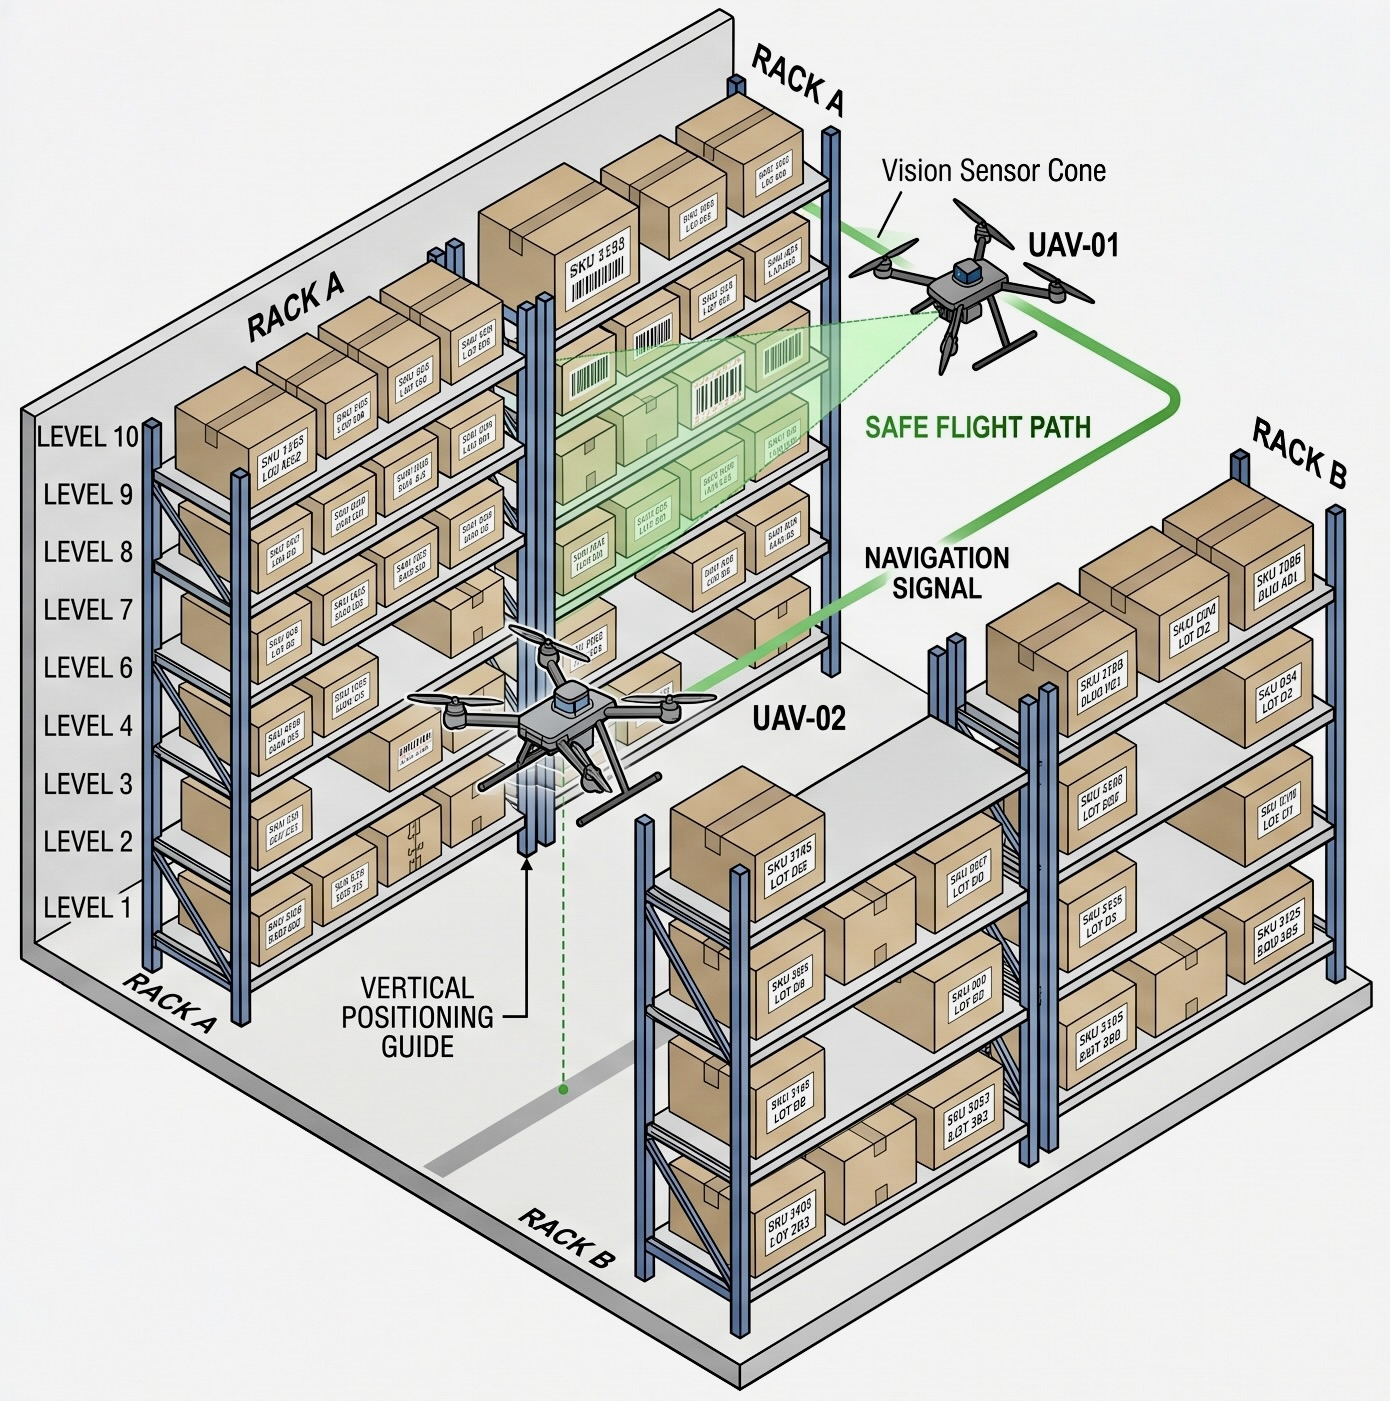
\includegraphics[width=0.4\textwidth]{Images/UAV1_UAV2_1.jpeg}
    \caption{Operazioni di volo e tracciamento multi-UAV.}
    \label{fig:warehouse_uav_operations}
\end{figure}

\newpage
Il rumore di processo, modellato come una variabile gaussiana a media nulla $\mathbf{w}_{t-1} \sim \mathcal{N}(0, \mathbf{Q})$, è fondamentale per introdurre l'incertezza intrinseca del volo, simulando perturbazioni esogene come le correnti d'aria trasversali generate dai rotori che i soli modelli matematici deterministici non possono prevedere \cite{Ye2023}.

Nello specifico del simulatore, la matrice di covarianza del rumore di processo $\mathbf{Q}$ è stata tarata sperimentalmente per bilanciare la fiducia che il filtro di Kalman (EKF) ripone nel modello cinematico rispetto alle misurazioni radio: un valore eccessivo di $\mathbf{Q}$ indicherebbe una totale imprevedibilità del drone, costringendo l'algoritmo ad affidarsi esclusivamente al segnale RF, mentre un valore troppo basso porterebbe l'EKF a ignorare i dati radio a favore di una stima puramente inerziale.

Oltre alla traslazione spaziale, un aspetto ingegneristico critico per i collegamenti direzionali 6G è l'orientamento dell'UAV. Per mantenere la posizione di hovering o eseguire manovre nei ristretti corridoi VNA, l'autopilota del drone deve costantemente variare il proprio assetto, modificando gli angoli di rollio ($\Phi$), beccheggio ($\Theta$) e imbardata ($\Psi$) \cite{Muller2024}. Queste rapide fluttuazioni dell'orientamento introducono un'incertezza significativa. Sebbene il drone utilizzi sensori inerziali (IMU) e un filtro EKF interno per stimare il proprio assetto, tali misurazioni sono affette da rumore termico e derive \cite{Muller2024}. Analisi sperimentali dimostrano che la stima degli angoli di Eulero tramite EKF presenta sempre un errore residuo (ad esempio, $\Phi_e, \Theta_e, \Psi_e$), che seppur confinato tipicamente entro incertezze espanse di $\pm0.3^\circ$, genera fluttuazioni microscopiche continue della piattaforma \cite{Muller2024}.

Dal punto di vista delle telecomunicazioni, le incertezze di orientamento del velivolo si ripercuotono con conseguenze potenzialmente catastrofiche sulla stabilità del Link Budget. Operando a frequenze elevate (come la banda 5.9 GHz simulata o le onde millimetriche), gli elementi radianti generano fasci (beam) dotati di estrema direttività spaziale. Qualora l'assetto del drone si inclini oltre le tolleranze di progetto, il fascio dell'antenna perde il puntamento ottimale verso il nodo ricevitore (BS o RIS), inducendo il deleterio fenomeno del Beam Misalignment (disallineamento del fascio).

Nel motore fisico del Digital Twin, questa meccanica di degradazione è stata quantificata e integrata nel loop di simulazione. Inizialmente, il sistema calcola l'errore angolare totale equivalente $\theta_{error}$ derivante dalle combinazioni di pitch e roll (vincolate per questioni di sicurezza indoor a un angolo massimo teorico di 15$^\circ$):

% Equazione 4.4: Errore angolare totale derivato dall'assetto (Beam Misalignment)
\begin{equation}
\theta_{error} = \sqrt{\Phi^2 + \Theta^2}
\label{eq:beam_angular_error}
\end{equation}

Successivamente, qualora tale incertezza d'assetto superi una guard-band angolare di tolleranza fissata a 5$^\circ$, il canale di propagazione subisce un'attenuazione additiva definita come Misalignment Loss ($L_{mis}$), la quale cresce linearmente al tasso di 0.5 dB per ogni grado di sforamento:

% Equazione 4.5: Modello di perdita per disallineamento (Beam Misalignment Loss)
\begin{equation}
L_{mis} = \max\left(0, (\theta_{error} - 5^\circ) \cdot 0.5 \right) \text{ dB}
\label{eq:beam_misalignment_loss}
\end{equation}

Questa severa penalizzazione da disallineamento -- il cui limite superiore (cap) è impostato a 15.0 dB -- si somma vettorialmente alla Penetration Loss degli ostacoli metallici calcolata nel motore di Ray-Casting. Nei casi più critici, l'effetto combinato di queste due attenuazioni può innescare un drammatico calo del rapporto segnale-rumore (SNR) al di sotto della soglia operativa di demodulazione, condannando il drone a repentine seppur temporanee disconnessioni dalla rete (outage) e mettendo in crisi le capacità predittive del filtro di tracciamento.


\subsection{Fusione Sensoriale EKF}

Il tracciamento autonomo di un UAV in un ambiente logistico indoor rappresenta una sfida ingegneristica complessa, specialmente quando il ricevitore a bordo è equipaggiato con una singola antenna (SISO). In tali condizioni operative, le misurazioni derivanti dai segnali radio (come RSRP e AoA) sono intrinsecamente degradate dal multipath fading, dall'attenuazione da blocco e dal rumore termico dinamico dei componenti attivi. Per ottenere una stima posizionale sub-metrica, accurata e continua, è indispensabile fondere i dati incerti provenienti dalle osservazioni elettromagnetiche con il modello cinematico di volo del drone.

A tale scopo, il Digital Twin sviluppato implementa un Extended Kalman Filter (EKF). L'EKF è un filtro ricorsivo Bayesiano sub-ottimo, progettato specificamente per gestire le non-linearità intrinseche dei sistemi dinamici complessi e dei modelli di osservazione spaziale \cite{Ye2023}. A differenza del Filtro di Kalman lineare standard, l'EKF linearizza localmente le funzioni non lineari calcolandone le derivate parziali tramite matrici Jacobiane ad ogni passo temporale. Dal punto di vista sistemistico, il filtro opera attraverso un ciclo iterativo perpetuo a 10 Hz, sincronizzato con il clock deterministico della simulazione ($T_s= 0.1$ s), suddiviso in due fasi fondamentali: Predizione (\textit{Predict}) e Aggiornamento (\textit{Update}) \cite{Ye2023}.

\subsubsection{Fase di Predizione e limite inerziale (Test 1: Coasting)}

Nella fase di Predizione, il filtro proietta lo stato precedente nel futuro basandosi esclusivamente sulle leggi della cinematica newtoniana (navigazione inerziale). Lo stato del sistema al tempo discreto $t$ è definito da un vettore a sei dimensioni:

% Equazione 4.6: Vettore di stato 6D
\begin{equation}
\mathbf{x}_t = [x, y, z, v_x, v_y, v_z]^T
\label{eq:ekf_state}
\end{equation}

La stima a priori dello stato $\hat{\mathbf{x}}_{t|t-1}$ viene calcolata attraverso la matrice di transizione di stato $\mathbf{F}$, che applica le equazioni del moto integrando la velocità nel tempo di campionamento $T_s$. Parallelamente, il filtro propaga l'incertezza calcolando la matrice di covarianza dell'errore a priori: 

% Equazione 4.7: Predizione della Covarianza dell'Errore
\begin{equation}
\mathbf{P}_{t|t-1} = \mathbf{F} \mathbf{P}_{t-1} \mathbf{F}^T + \mathbf{Q}
\label{eq:ekf_prior_cov}
\end{equation}

In questa equazione, $\mathbf{Q}$ rappresenta la matrice di covarianza del rumore di processo, che modella le perturbazioni fisiche esogene e non deterministiche (come le turbolenze aerodinamiche sui rotori). Nel simulatore, $\mathbf{Q}$ è tarata con un coefficiente di 0.1, bilanciando la fiducia del filtro verso il modello matematico del volo \cite{Ye2023}.

\subsubsection{Fase di Aggiornamento e Assisted-LoS (Test 2: Innovation Step)}

Il salto tecnologico evidenziato nel Test 2 avviene tramite l'introduzione di RIS attive, le quali instaurano un percorso in visibilità assistita (Assisted-LoS). Quando l'SNR calcolato dal Link Budget supera la soglia operativa di 5 dB, il sistema incorpora le misurazioni radio ricevute in tempo reale ed esegue la fase di Aggiornamento.

Il vettore di osservazione $\mathbf{z}_t$ contiene le coordinate spaziali 3D derivate dalla multilaterazione del segnale RF. Poiché la relazione $h(\mathbf{x})$ tra il segnale ricevuto e la posizione spaziale è non lineare, l'EKF linearizza il problema calcolando la matrice Jacobiana dell'osservazione:

% Equazione 4.8: Matrice Jacobiana dell'osservazione
\begin{equation}
\mathbf{H}_t = \frac{\partial h}{\partial \mathbf{x}} \bigg|_{\mathbf{x}=\hat{\mathbf{x}}_{t|t-1}}
\label{eq:ekf_jacobian}
\end{equation}

Il cuore matematico della correzione risiede nel calcolo del Guadagno di Kalman (Kalman Gain, $\mathbf{K}_t$), il quale agisce come un fattore di peso che decide se "fidarsi" maggiormente della predizione inerziale o della misurazione radio:

% Equazione 4.9: Calcolo del Guadagno di Kalman
\begin{equation}
\mathbf{K}_t = \mathbf{P}_{t|t-1} \mathbf{H}_t^T (\mathbf{H}_t \mathbf{P}_{t|t-1} \mathbf{H}_t^T + \mathbf{R}_t)^{-1}
\label{eq:ekf_kalman_gain}
\end{equation}

Il parametro critico è $\mathbf{R}_t$, la matrice di covarianza del rumore di misura. Nel Digital Twin, $\mathbf{R}_t$ è dinamica: viene impostata a valori elevati (es. 2.0) in NLoS per riflettere l'estrema inaccurattezza delle letture ostruite, mentre crolla a valori minimi quando le RIS creano un Assisted-LoS pulito.

Infine, lo stato a posteriori (la stima finale) viene aggiornato aggiungendo il residuo di misurazione pesato (l'\textit{Innovation Step}), "ancorando" il drone alla realtà fisica: 

% Equazione 4.10: Aggiornamento dello Stato a posteriori
\begin{equation}
\hat{\mathbf{x}}_t = \hat{\mathbf{x}}_{t|t-1} + \mathbf{K}_t (\mathbf{z}_t - h(\hat{\mathbf{x}}_{t|t-1}))
\label{eq:ekf_posterior_state}
\end{equation}

Contestualmente, la matrice di covarianza viene ristretta, abbattendo visivamente l'ellisse di incertezza spaziale:

% Equazione 4.11: Aggiornamento della Covarianza a posteriori
\begin{equation}
\mathbf{P}_t = (\mathbf{I} - \mathbf{K}_t \mathbf{H}_t) \mathbf{P}_{t|t-1}
\label{eq:ekf_posterior_cov}
\end{equation}

L'esecuzione di questo reintegro dei residui annulla istantaneamente la deriva inerziale accumulata durante il coasting.

\subsubsection{Monitoraggio RMSE e Interrupt di Collisione}

A livello di sicurezza del software, per garantire l'incolumità intrinseca della navigazione, ad ogni ciclo di clock il motore estrae il Root Mean Square Error (RMSE), calcolando la norma euclidea tra le coordinate reali (Ground Truth) e la stima dell'EKF:

% Equazione 4.12: Calcolo dell'RMSE spaziale
\begin{equation}
\text{RMSE}(t) = \|\mathbf{p}_{real}(t) - \mathbf{\hat{p}}_{est}(t)\|_2
\label{eq:ekf_rmse}
\end{equation}

Qualora questo scarto superi la soglia critica di tolleranza spaziale (impostata a 1.5 m), l'algoritmo innesca un Interrupt interrogando l'albero KD-Tree degli ostacoli, rilevando la collisione imminente e decretando il fallimento della missione.
\subsection{Controller SDN e i suoi Algoritmi}

In un ecosistema ad alta densità informativa quale la futura rete 6G, l'infrastruttura Software-Defined Networking (SDN) centralizzata assume il ruolo di intelligenza suprema del network. Tale paradigma consente il disaccoppiamento critico tra il Control Plane (livello logico decisionale) e il Data Plane (hardware trasmissivo fisico), garantendo una flessibilità operativa indispensabile. Le mansioni dell'orchestratore SDN nel Digital Twin sviluppato non si esauriscono nella gestione radiopropagativa a run-time, ma costituiscono la base analitica per il setup fisico iniziale, agendo sulla pianificazione della Bill of Materials (BOM) e sull'allocazione topologica dei nodi.

\begin{figure}[H]
    \centering
    \resizebox{0.85\textwidth}{!}{
    \begin{tikzpicture}[
        auto,
        font=\sffamily\small,
        block/.style = {rectangle, draw=blue!60, fill=blue!5, thick, text width=3cm, text centered, rounded corners, minimum height=1.2cm},
        ai_block/.style = {rectangle, draw=green!60!black, fill=green!5, thick, text width=3.5cm, text centered, rounded corners, minimum height=1.2cm},
        ekf_block/.style = {rectangle, draw=orange!80, fill=orange!5, thick, text width=3.5cm, text centered, rounded corners, minimum height=1.2cm},
        hardware/.style = {rectangle, draw=gray!80, fill=gray!10, thick, text width=3cm, text centered, minimum height=1cm},
        line/.style = {draw, thick, ->, -{Stealth[scale=1.2]}},
        dashed_line/.style = {draw, thick, dashed, ->, -{Stealth[scale=1.2]}},
        background_ekf/.style = {rectangle, fill=orange!10, rounded corners, draw=orange!50, dashed, inner sep=0.3cm},
        background_lstm/.style = {rectangle, fill=green!10, rounded corners, draw=green!60!black, dashed, inner sep=0.3cm}
    ]
    
    % Nodes
    \node [block, fill=magenta!10, draw=magenta] (oran) {\textbf{O-RAN Interface}\\(E2 Node)};
    \node [block, right=1cm of oran] (telemetry) {\textbf{Metriche Grezze}\\AoA, RSSI, IMU};
    
    \node [coordinate, right=0.8cm of telemetry] (split) {};
    
    % EKF Path (Top)
    \node [ekf_block, above right=0.5cm and 0.5cm of split] (ekf_predict) {\textbf{EKF Predict}\\Stima Cinematica\\(Inerziale)};
    \node [ekf_block, right=1.2cm of ekf_predict] (ekf_update) {\textbf{EKF Update}\\Innovazione Radio\\(Assisted-LoS)};
    
    \node [block, right=1.2cm of ekf_update, fill=cyan!10, draw=cyan!80!black] (position) {\textbf{Stima Posizione}\\(Sub-metrica)};
    
    % LSTM Path (Bottom)
    \node [ai_block, below right=0.5cm and 0.5cm of split] (lstm) {\textbf{Memoria LSTM}\\Analisi Storico};
    \node [ai_block, right=1.2cm of lstm] (predict_curve) {\textbf{Predizione Curva $90^\circ$}\\(Superamento Coasting)};
    
    \node [block, right=1.2cm of predict_curve, fill=purple!10, draw=purple] (ris_ctrl) {\textbf{SDN Orchestrator}\\Make-Before-Break};
    
    % Backgrounds
    \begin{scope}[on background layer]
        \node[background_ekf, fit=(ekf_predict) (ekf_update), label=above:\textbf{Filtro EKF}] (ekf_bg) {};
        \node[background_lstm, fit=(lstm) (predict_curve), label=below:\textbf{Intelligenza Artificiale (LSTM)}] (lstm_bg) {};
    \end{scope}
    
    % Hardware interaction
    \node [hardware, above=2cm of ekf_update, fill=green!15, draw=green!60!black] (ris_active) {\textbf{RIS Corrente}\\(Stato: ACTIVE)};
    \node [hardware, right=1.5cm of ris_active, fill=red!15, draw=red!80] (ris_next) {\textbf{RIS Target}\\(Stato: SLEEP $\rightarrow$ ACTIVE)};
    
    % Edges
    \path [line] (oran) -- (telemetry);
    \path [draw, thick] (telemetry) -- (split);
    \path [line] (split) |- (ekf_predict);
    \path [line] (split) |- (lstm);
    
    \path [line] (ekf_predict) -- node {$\mathbf{\hat{x}}_{t|t-1}$} (ekf_update);
    \path [line] (ekf_update) -- node {$\mathbf{\hat{x}}_t$} (position);
    
    \path [line] (lstm) -- node[above] {Pattern} (predict_curve);
    \path [line] (predict_curve) -- node[above] {$\Delta t$ Anticipo} (ris_ctrl);
    
    % Cross interactions
    \path [line, dashed, blue!80!black] (position.south) -- ++(0,-0.6) -| node[pos=0.25, above, font=\scriptsize] {Feed Posizionale} (lstm.north);
    \path [line] (ris_active) -- node[left, font=\scriptsize] {Link Radio} (ekf_update);
    \path [dashed_line, color=red!80!black, very thick] (ris_ctrl.east) -- ++(1.5,0) |- node[pos=0.25, right, font=\scriptsize, align=center] {Comando di\\Wake-Up} (ris_next.east);
    
    \end{tikzpicture}
    }
    \caption{Diagramma di Flusso della Fusione Sensoriale Ibrida. Il sistema orchestra parallelamente l'elaborazione inerziale sub-metrica tramite Extended Kalman Filter (EKF) e la mappatura predittiva spazio-temporale della rete neurale (LSTM), anticipando l'attivazione della RIS successiva (Make-Before-Break).}
    \label{fig:hybrid_ekf_lstm}
\end{figure}

\subsubsection{Deployment Topologico NLoS e Algoritmi di Clustering K-Means}

Negli ambienti di logistica industriale, le scaffalature Very Narrow Aisle (VNA) costituiscono barriere invalicabili per le alte frequenze (strutture in acciaio ad elevato assorbimento). Il posizionamento esatto delle superfici RIS è dunque un problema di ottimizzazione spaziale, affrontato nel simulatore tramite il Test 0 (BOM \& K-Means Deployment).

Per determinare le coordinate cartesiane ottimali, l'architettura SDN esegue un preventivo vettorializzamento ad "ombre radianti". Mappando l'ambiente, il sistema calcola una densa Point-Cloud rappresentante le regioni in stato di Non-Line-of-Sight (NLoS) severo. Una volta strutturata la mappa, viene implementato l'algoritmo K-Means. Il sistema aggrega i punti della nuvola riducendoli a un numero finito $K$ di cluster, dove $K$ coincide con la disponibilità hardware di pannelli RIS. L'algoritmo minimizza iterativamente la varianza spaziale intra-cluster per identificare i baricentri operativi $\mu_i$:

% Equazione 4.13: Funzione obiettivo del K-Means
\begin{equation}
J = \sum_{i=1}^{K} \sum_{x \in S_i} \|x - \mu_i\|^2
\label{eq:kmeans_objective}
\end{equation}

Per rendere i risultati applicabili industrialmente, l'SDN integra un approccio di tassellazione Greedy: le coordinate teoriche vengono vincolate calcolando la distanza ortogonale più breve verso la paratia o il soffitto più vicino, fissando l'altezza al 95\% dell'asse Z per massimizzare l'illuminazione Top-Down. Tale logica scala agilmente da configurazioni minime per hub di 2.000 m$^2$ fino a deployment densi di 24 array per macro-hub da 35.000 m$^2$.

\subsubsection{Limiti dell'Inerzia e Analisi di Transitorio Neurale (LSTM)}

Se il filtro EKF (Capitolo 4.2) gestisce efficacemente il jitter in tratti lineari, esso fallisce drasticamente di fronte alle curve a 90$^\circ$ dei corridoi VNA a causa della sua natura markoviana e localmente linearizzata. In assenza di segnale radio (NLoS), l'EKF entra in Coasting, portando il drone a divergere dalla traiettoria reale (Ground Truth).

Per rimediare a tale collasso, l'SDN introduce il criterio di Trajectory Prediction tramite reti neurali Long Short-Term Memory (LSTM) residenti a livello Edge. A differenza dell'algebra lineare dell'EKF, i Memory Gate dell'LSTM elaborano l'intero storico vettoriale del moto, catturando le interdipendenze non lineari e anticipando i reali angoli di sterzata con precisione millimetrica prima che la manovra avvenga fisicamente \cite{Zhang2022}.

\subsubsection{Soppressione della Blind Reflection e Controllo ON-OFF}

L'integrità del Layer elettromagnetico richiede un controllo dinamico dell'attivazione. Mantenere 24 array RIS in modalità Always-ON genererebbe "riflessioni cieche" (blind reflections), innalzando il rumore di fondo e facendo collassare il SINR (Signal-to-Interference-plus-Noise Ratio).

L'SDN istruisce il controllore mediante un Vettore di Attivazione binario $\mathbf{V}$:

% Equazione 4.14: Vettore binario di attivazione RIS
\begin{equation}
\mathbf{V} = \{v_1, v_2, \dots, v_R\}, \quad v_i \in \{0, 1\}
\label{eq:ris_activation_vector}
\end{equation}

dove $v_i = 1$ commuta la RIS in Active Mode (50 W) e $v_i = 0$ la confina in Sleep Mode (0.5 W). Il calcolo del SINR formale ($\gamma_l$) per l'utente target $l$ viene così ottimizzato \cite{Zhang2022}:

% Equazione 4.15: SINR in presenza di Multi-RIS e Blind Reflection
\begin{equation}
\gamma_l = \frac{P \left| \sqrt{\eta_l}g_l + \sum_{i=1}^{R} \sqrt{\eta_{l,i}} v_i h_i \Phi_i h_{l,i} \right|^2}{P \left| \sum_{m=1}^{U_I} \sqrt{\eta_m}g_m + \sum_{i=1}^{R} \sqrt{\eta_{m,i}} v_i h_i \Phi_i h_{m,i} \right|^2 + \sigma^2}
\label{eq:sinr_blind_reflection}
\end{equation}

Questa logica abilita il paradigma Make-Before-Break: l'SDN, leggendo la predizione LSTM, invia un comando di Wake-Up alla RIS necessaria con un anticipo di $\Delta t = 100$ ms. Tale approccio "Zero-Latency-Equivalent" permette di mantenere l'RMSE $\le 1.0$ m anche in presenza di pesanti ritardi di Backhaul ($> 250$ ms).
\subsection{Architettura Software e Ottimizzazione Energetica}

Lo sviluppo di un sistema Digital Twin ad elevatissime prestazioni, destinato a governare ambienti indoor ad alta mobilità per reti 6G, esige -- parallelamente alla complessa algebra formale finora descritta -- un'infrastruttura di elaborazione software votata alla computazione massicciamente parallela. Il controller SDN non gestisce veri cicli sequenziali, ma fonde la vettorializzazione spaziale per il ray-tracing ottico, il ricalcolo matriciale dello stato nell'Extended Kalman Filter (EKF) e gli algoritmi di ottimizzazione energetica RF. Tale mole logica deve essere evasa in finestre temporali stringenti, rigorosamente inferiori alla soglia critica della latenza di controllo ($< 10$ ms).

\subsubsection{Oltre il Threading: Bypass del GIL e IPC in Zero-Copy}

Il linguaggio di elezione per l'ingegnerizzazione dell'orchestrazione neurale (Machine Learning) e dei backend SDN è tipicamente Python, apprezzato per la sua sterminata versatilità. Tuttavia, l'interprete standard (CPython) è vincolato dal noto Global Interpreter Lock (GIL). Questo mutex architettonico proibisce la reale esecuzione concorrente-parallela in architetture Multithreading, forzando il partizionamento seriale dei cicli di esecuzione su un singolo core logico. Sottoporre a questo vincolo i colossali pesi computazionali del filtraggio radar 3D genererebbe starvation delle risorse e asincronie fatali.

Per eradicare questa paralisi asincrona, l'infrastruttura del simulatore è stata ingegnerizzata adottando il paradigma del Multiprocessing, integrato ai costrutti di gestione della memoria a basso livello tipici dei sistemi operativi POSIX (\texttt{SharedMemoryAllocator}). Evitando le inefficienze dei passaggi di stato tramite serializzazioni software standard (come code logiche I/O o le sovrastrutture in JSON evidenziate in \cite{Vairam2023}), l'architettura alloca nativamente un segmento persistente in RAM condivisa.

I tensori vettoriali (tra cui il vettore di stato $\mathbf{X}_t$) e le complesse matrici di fase della RIS sono strutturati al limite stringente degli array C-like. I processi paralleli -- in particolare il Control Plane (decisionale) e il Data Plane (fisico-radiante) -- operano in lettura e scrittura simultanea tramite estrazione Zero-Copy. Questo stratagemma architetturale azzera il mastodontico overhead di conversione tipico della Inter-Process Communication (IPC), riducendo le latenze di interscambio allo stato dell'arte (frazioni di sub-nanosecondo netto).

\subsubsection{Strutture ad Albero (KD-Tree) e Compilazione JIT (LLVM Numba)}

Laddove la rete gestisce la modellazione fisica radiopropagativa 3GPP InF-DH (Indoor Factory), emerge l'ostruzionismo geometrico inerente alla verifica dello stato Line-of-Sight (LoS) e al calcolo vettoriale della Penetration Loss (NLoS). In ogni iterazione (Time-Step $t$), il motore analitico deve risolvere l'intersezione della retta parametrica $\vec{r}(t)$ passante tra emittente e ricevente:

% Equazione 4.16: Equazione parametrica del raggio radio per il Ray-Casting vettorializzato
\begin{equation}
\vec{r}(t) = \mathbf{p}_{tx} + t \cdot \vec{d}_{dir}
\label{eq:ray_casting_parametric}
\end{equation}

Poiché le ostruzioni volumetriche (scaffalature VNA) sono modellate come matrici AABB (Axis-Aligned Bounding Box), un approccio computazionale iterativo a forza bruta (brute-force) manderebbe in stallo la CPU, presentando una complessità quadratica asintoticamente ingestibile ad alta scalabilità. Tale limite viene risolto strutturando lo spazio logistico in un partizionamento gerarchico standardizzato tramite alberi KD-Tree. La suddivisione spaziale abilita l'esclusione binaria di tutti i rami non intersecanti il raggio, de-escalando drasticamente la logica iterativa dalla scala lineare $\mathcal{O}(N)$ a una ben più snella complessità $\mathcal{O}(\log N)$.

Parallelamente, per colmare la latenza del calcolo matriciale tipico dei cicli \textit{for-loop} di Python (rallentati dal \textit{duck-typing} nativo), l'intera routine geometrica di Ray-Casting è stata demandata al framework Numba tramite compilazione Just-In-Time (JIT). Applicando il decoratore \texttt{@njit(nogil=True)}, all'inizializzazione del codice il back-end LLVM traduce i costrutti analitici direttamente in rigoroso linguaggio macchina C. Questa duplice sinergia informatica scavalca in toto le dipendenze del GIL, accelerando vertiginosamente lo strato matematico reattivo: i collaudi sperimentali certificano un incremento brutale delle prestazioni nell'ordine di due magnitudini ($\sim 100\times$).

\begin{figure}[H]
    \centering
    \begin{tikzpicture}[scale=0.68, every node/.style={transform shape},
        font=\sffamily\small,
        process/.style  = {rectangle, draw=blue!70!black, fill=blue!8, thick, rounded corners, minimum width=4.5cm, minimum height=3.8cm, inner sep=0.3cm},
        shmem/.style    = {rectangle, draw=teal!80!black, fill=teal!10, thick, rounded corners, minimum width=3.2cm, minimum height=3.8cm, inner sep=0.3cm},
        module/.style   = {rectangle, draw=orange!80!black, fill=orange!8, thick, rounded corners, text width=3.5cm, align=center, minimum height=0.9cm},
        jit_mod/.style  = {rectangle, draw=red!70!black, fill=red!8, thick, rounded corners, text width=3.5cm, align=center, minimum height=0.9cm},
        mem_block/.style= {rectangle, draw=teal!80!black, fill=teal!20, thick, rounded corners, text width=2.6cm, align=center, minimum height=0.9cm},
        ipc/.style      = {draw, very thick, <->, -{Stealth[scale=1.2]}, color=teal!70!black},
        gil_cross/.style= {draw=red!80!black, very thick, double},
        gil_label/.style= {font=\sffamily\bfseries\tiny, text=red!80!black},
        head_label/.style={font=\sffamily\bfseries, text=white},
        layer_bg/.style = {rectangle, fill=gray!10, rounded corners, draw=gray!40, dashed, inner sep=0.25cm}
    ]

    % --- PROCESS A: Data Plane (Physics Engine) ---
    \node[process, label={[font=\sffamily\bfseries\small, text=blue!70!black]above:\textbf{Processo A — Data Plane}}] (procA) at (0,0) {};

    \node[module] (kdtree)  at (0,  1.2) {\textbf{KD-Tree Spatial Index}\\ $\mathcal{O}(\log N)$ Ray-Cast};
    \node[jit_mod](jit_ray) at (0,  0.1) {\textbf{@njit(nogil=True)}\\ LLVM Ray-Casting};
    \node[module] (physics) at (0, -1.0) {\textbf{Physics Engine}\\ Path Loss / SNR};
    \node[module] (sampler) at (0, -2.0) {\textbf{Sensor Sampler}\\ GFRA Telemetry 10 Hz};

    % GIL Cross-out badge on procA
    \node[draw=red!80!black, fill=red!15, thick, rounded corners, font=\sffamily\bfseries\tiny, text=red!80!black,
          inner sep=2pt] at (procA.north east) {GIL-FREE};

    % --- SHARED MEMORY (Centre) ---
    \node[shmem, label={[font=\sffamily\bfseries\small, text=teal!70!black]above:\textbf{Shared Memory (POSIX)}}] (shmem) at (6.5, 0) {};

    \node[mem_block] (st_vec)    at (6.5,  1.4) {\textbf{State Vector} $\mathbf{X}_t$ ~~[6$\times$1 f64]};
    \node[mem_block] (ris_mat)   at (6.5,  0.3) {\textbf{RIS Phase Matrix} ~~[$N{\times}N$ cpx]};
    \node[mem_block] (snr_buf)   at (6.5, -0.8) {\textbf{SNR Ring-Buffer} ~~[float32 x 256]};
    \node[mem_block] (ctrl_flag) at (6.5, -1.9) {\textbf{Control Flags} ~~[atomic uint8]};

    % Zero-Copy badge
    \node[draw=teal!80!black, fill=teal!25, thick, rounded corners, font=\sffamily\bfseries\tiny,
          text=teal!90!black, inner sep=2pt] at (shmem.north east) {ZERO-COPY};

    % --- PROCESS B: Control Plane (SDN/EKF) ---
    \node[process, label={[font=\sffamily\bfseries\small, text=blue!70!black]above:\textbf{Processo B — Control Plane}}] (procB) at (13, 0) {};

    \node[module] (ekf)    at (13,  1.2) {\textbf{EKF Tracking Engine}\\ Jacobiani 6D};
    \node[jit_mod](jit_ekf)at (13,  0.1) {\textbf{@njit(nogil=True)}\\ LLVM Matrix Inversion};
    \node[module] (lstm_b) at (13, -1.0) {\textbf{LSTM Predictor}\\ Trajectory 10-step};
    \node[module] (sdn_b)  at (13, -2.0) {\textbf{SDN Orchestrator}\\ RIS ON/OFF Logic};

    \node[draw=red!80!black, fill=red!15, thick, rounded corners, font=\sffamily\bfseries\tiny, text=red!80!black,
          inner sep=2pt] at (procB.north east) {GIL-FREE};

    % --- IPC ARROWS ---
    \draw[ipc] (procA.east) -- (shmem.west)
        node[midway, above, font=\sffamily\scriptsize, text=teal!80!black] {Write}
        node[midway, below, font=\sffamily\scriptsize, text=gray!70] {sub-ns latency};

    \draw[ipc] (shmem.east) -- (procB.west)
        node[midway, above, font=\sffamily\scriptsize, text=teal!80!black] {Read}
        node[midway, below, font=\sffamily\scriptsize, text=gray!70] {sub-ns latency};

    % --- CLOCK LABEL ---
    \node[draw=purple!80, fill=purple!10, rounded corners, thick,
          font=\sffamily\scriptsize\bfseries, text=purple!80!black,
          text width=6cm, align=center, inner sep=4pt] at (6.5, -3.2)
        {\textbf{Simulation Clock} \\ $\Delta t = 100\,\text{ms}$ --- 10 Hz \\ Deterministico e Sincronizzato};

    \draw[->, thick, purple!70!black, dashed] (6.5,-2.9) -- (6.5,-2.5);

    \end{tikzpicture}
    \caption{Architettura Software del Digital Twin: Bypass del GIL tramite Multiprocessing e comunicazione Zero-Copy. Il Processo A (Data Plane) esegue il Ray-Casting vettorializzato con KD-Tree e compilazione JIT Numba. Il Processo B (Control Plane) aggiorna le matrici EKF e orchestra le predizioni LSTM. I due processi condividono tensori di stato tramite un segmento POSIX Shared Memory ad accesso diretto (Zero-Copy), azzerando la latenza IPC convenzionale.}
    \label{fig:software_arch_zero_copy}
\end{figure}

\subsubsection{Risoluzione di Dinkelbach e Transizione "Green 6G" (BD-RIS)}

Questa potentissima e abilitante ingegneria dei flussi sposta il reale focus dell'elaboratore verso il traguardo dell'Ottimizzazione Energetica. Le normative della logistica cooperativa moderna impongono, parallelamente alle prestazioni in banda, un severo regime operativo "Green 6G". È qui esplicitato il requisito del minimo impatto termico, conseguito instradando in Sleep Mode (standby passivo) la porzione ridondante dell'infrastruttura RIS per azzerare l'inquinamento spettrale (Spectrum Pollution).

L'obiettivo formale univoco è il conseguimento del picco di Efficienza Energetica Assoluta (AEE). Tale metrica si analizza come il rapporto tra il Data Rate massimo fruibile ($R_s$) e la potenza totale esigita dal network ($P_{tot}$), intesa come la somma della potenza emissiva radiante in Base-Station ($P_s$) e il consumo cumulativo elettronico ausiliario dei circuiti hardware RIS in ascolto ($P_c$).

La modellizzazione rigorosa di tale vincolo incastra l'architettura logica nel dominio della massimizzazione frazionaria non convessa:

% Equazione 4.17: Modello originario della massimizzazione dell'Efficienza Energetica Assoluta (AEE)
\begin{equation}
\max_{P_s, \Theta} \frac{R_s}{P_s + P_c}
\label{eq:aee_maximization}
\end{equation}

Tentare una risoluzione euristica diretta (per forza bruta) su un piano refrattario di tale complessità implicherebbe cicli ricorsivi lenti, vanificando le scadenze Real-Time e rendendo impraticabile l'intero sistema 6G. Per abbattere il vicolo cieco del quoziente, il Controller SDN fa appello in codice sorgente all'elegante espediente iterativo lineare noto in dottrina come Metodo di Dinkelbach \cite{Khan2024}.

Il sistema introduce l'incognita ausiliaria dinamica $\lambda$ (il moltiplicatore dell'efficienza ottimale di rete iterata). Tale manipolazione traslittera ed aliena il rapporto algebrico frazionale, riconfigurandolo rigorosamente nell'esatta forma equivalente sintetica e di natura strettamente concava:

% Equazione 4.18: Trasformazione lineare convessa mediante il Metodo di Dinkelbach
\begin{equation}
\max_{P_s, \Theta} R_s - \lambda(P_s + P_c)
\label{eq:dinkelbach_transformation}
\end{equation}

Librato formalmente dai gravosi limiti espliciti del denominatore al quoziente, il problema di integrazione procede fluidamente, calcolando la soluzione in due step di Ottimizzazione Alternata. Nel primo passaggio metodologico, s'intercetta l'ottimizzazione del vettore di energia emissiva $P_s$ tramite le Condizioni di Karush-Kuhn-Tucker (KKT) e il modello Lagrangiano. A consolidamento concluso, s'ottimizza incisivamente la complessa distribuzione matriciale del controllo di fase $\Theta$ (sfruttando gli asset della Varietà di Stiefel) \cite{Khan2024}.

La risultante congiunta, espletata dal simulatore JIT Python e chiusa termodinamicamente dal processo di Dinkelbach, spinge forzosamente in convergenza millimetrica la complessa matrice di tracciamento. I log-run fenomenologici estratti dai dataset metrici provano come l'algoritmo assesti rigidamente la rete sul vertice della curva Pareto-ottimale in assoluta tolleranza zero.

Infine, le evidenze simulatorie sanciscono l'indispensabilità di integrare l'architettura riflettente di frontiera Beyond-Diagonal RIS (BD-RIS) \cite{Khan2024}. Il passaggio dai vetusti modelli Diagonal-RIS (D-RIS) alla tecnologia Beyond-Diagonal garantisce non solo un tracciato sub-metrico col minimo consumo strutturale di safety-run, ma istituisce formalmente l'hardware di riferimento insindacabile per l'operatività massiccia del futuro dominio applicato Green 6G.
\subsection{Architettura Logica del Server Centrale SDN: Il Digital Twin}

Il cuore computazionale dell'intero Digital Twin sviluppato per questa tesi risiede nel Server Centrale SDN (Software-Defined Networking). Progettare un sistema di tracciamento 6G indoor capace di gestire droni ad alta mobilità (raggiungendo i 3 m/s) e reti riflesse complesse (tramite BD-RIS) ha richiesto l'abbandono dei paradigmi di rete tradizionali fortemente decentralizzati.

Nel mio elaborato ho scelto di adottare un'architettura SBA (Service-Based Architecture), separando in modo netto il piano di trasmissione a radiofrequenza (Data Plane) dall'intelligenza decisionale (Control Plane), concentrando quest'ultima all'interno del controllore centrale SDN. A livello software, per garantire un'esecuzione real-time ed evitare i ben noti colli di bottiglia imposti dal GIL (Global Interpreter Lock) del linguaggio Python, il server è fondato su una rigorosa astrazione a multiprocesso. La comunicazione tra i moduli avviene a livello di hardware fisico allocato in RAM tramite Shared Memory, garantendo alle pipeline di scambiarsi enormi array multidimensionali (\textit{NumPy array}) di coordinate e matrici di fase con latenze intra-componente pressoché nulle.

Come schematizzato nella visione d'insieme dell'architettura di sistema (Figura \ref{fig:sdn_server_arch}), il Server SDN risulta diviso in sei macro-moduli paralleli, ognuno con una precisa responsabilità ingegneristica.

\begin{figure}[H]
    \centering
    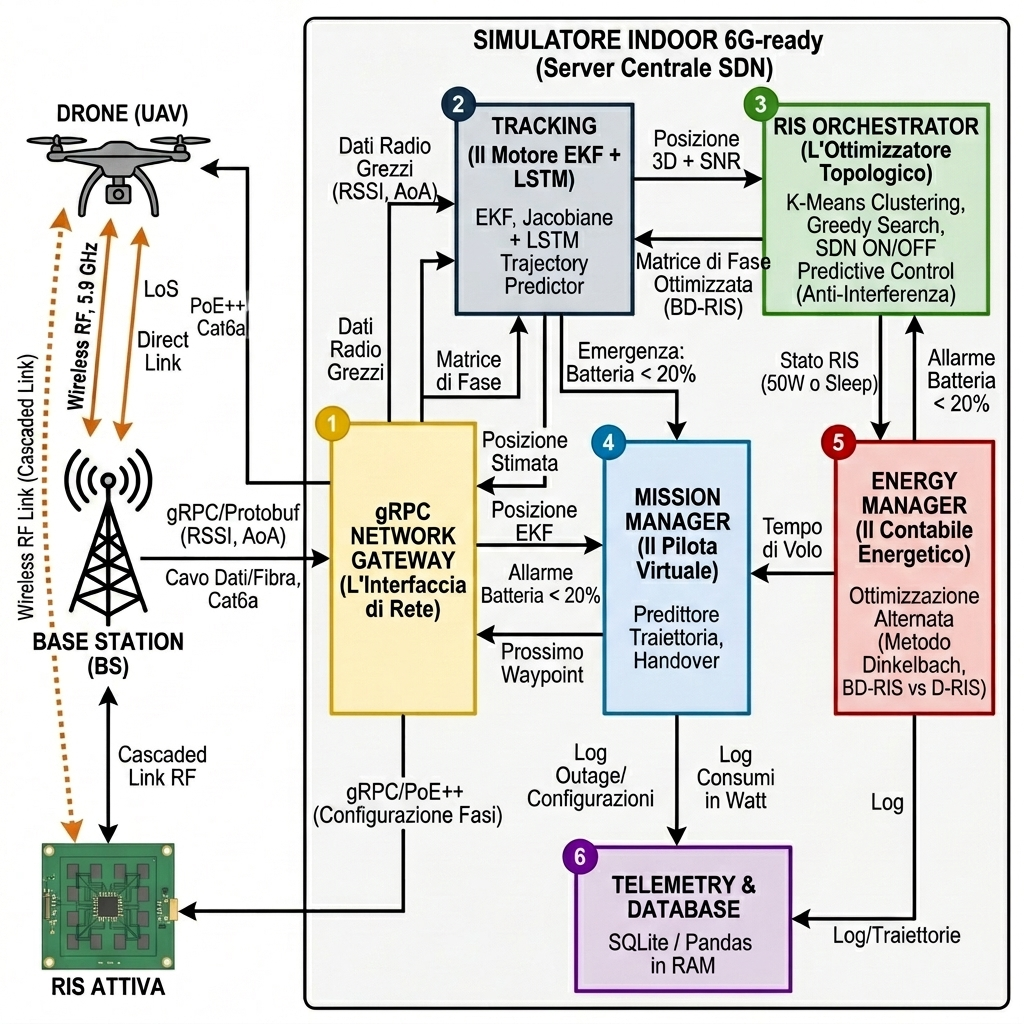
\includegraphics[width=0.85\textwidth]{../SDN_Server_Architecture_Updated.png}
    \caption{Dettaglio dell'Architettura Logica del Server Centrale SDN e dei suoi macro-moduli interni.}
    \label{fig:sdn_server_arch}
\end{figure}

\subsubsection{gRPC Network Gateway (Interfaccia di Rete)}

Il primo livello architetturale con cui interloquisce il livello fisico è l'Interfaccia di Rete, o Gateway. La funzione primaria di questo blocco è quella di agire come un broker bidirezionale: modella logicamente la connessione backhaul (es. cablaggi in fibra o Cat6a in PoE++) che intercorre tra i piloni centrali della Base Station e il server vero e proprio.

Durante le simulazioni, questo modulo ha un compito critico: deve gestire l'ingestione della telemetria passiva grezza, che nel nostro scenario industriale è rappresentata prevalentemente da vettori di misurazione RSSI (Received Signal Strength Indicator) e AoA (Angle of Arrival) dei fronti d'onda incidenti sulla BS. Essendo un Digital Twin orientato alla valutazione di una possibile implementazione reale, il Gateway gestisce anche l'incapsulamento logico Protobuf (protocol buffers tipici delle architetture gRPC) e l'iniezione temporale. Nello specifico, quando nel ``Test 3'' si voleva valutare il disallineamento indotto dalla rete ritardata (Beam Misalignment), è stato proprio il macro-blocco di rete a trattenere intenzionalmente pacchetti per 50 ms nella coda asincrona prima di rilasciarli ai livelli superiori, introducendo lo stress temporale controllato alla latenza della rete 6G.

\subsubsection{Tracking Engine (Motore EKF e Predizione Neurale)}

Acquisiti i dati grezzi dal livello Gateway, essi vengono instradati a larghissima banda verso il nucleo nevralgico della localizzazione spaziale: il Tracking Engine. Sviluppare un tracciatore puro basato solo sul Time of Flight o RSSI nudo non sarebbe stato proponibile a causa degli enormi jitter e del rumore moltiplicativo caratteristico degli ambienti indoor VNA densi di lamiere.

Per mitigare ciò, ho implementato operativamente un Modello Lineare-Quadratico basato sull'Extended Kalman Filter (EKF). L'algoritmo discretizza lo spettro temporale (a un tick $dt = 0.1$ s) e si occupa di generare le matrici Jacobiane per la fusione vettoriale (Data Fusion). Fonde la predizione statuale della cinematica intrinseca del drone (basata su equazioni differenziali newtoniane di massa e accelerazione) con l'aggiornamento dei residui ottenuti dalla rete. Fintanto che il legame di Line-of-Sight permane, l'EKF schiaccia drasticamente le curve di rumore, chiudendo costantemente l'errore metrico RMS entro tolleranze inferiori al metro e restringendo in tempo reale la propria matrice di covarianza d'incertezza ($P$).

Tuttavia, come validato sperimentalmente nella tesi, l'EKF possiede un punto critico: nelle manovre brusche dietro blocchi metallici in cui il segnale si azzera, l'EKF entra in ``Coasting''. Esegue previsioni solo tramite la sua componente inerziale-cinematica che, essendo approssimata linearmente, sfocia inevitabilmente a collidere autonomamente gli array contro le scaffalature metalliche entro pochi decimi di secondo.

Per compensare strutturalmente questo limite e fornire robustezza al delay di rete, all'interno dello stesso Engine ho inserito in maniera evolutiva l'integrazione con un Predittore di Traiettoria basato su architettura Deep Learning (LSTM - Long Short-Term Memory). La componente neurale LSTM intercetta non l'ultimo stato, ma la finestra cronologica storica delle ultime coordinate EKF pulite. I \textit{gate} di memoria riescono quindi ad assimilare la derivata spaziale non lineare associata al momento inerziale di virata del drone: prima ancora che subentri l'oblio d'aggiornamento del NLoS, la rete spinge sul bus la proiezione equivalentemente a ``Zero Latenza'', fornendo un oracolo spaziale (es. $t + 50$ ms) essenziale per le funzioni preventive.

\subsubsection{RIS Orchestrator (L'Ottimizzatore Topologico)}

I dati tridimensionali puliti dal Tracking Engine fluiscono sincronicamente dentro il RIS Orchestrator. Al contrario dell'approccio Wi-Fi standard in cui i router irradiano ciecamente a $360^\circ$, l'approccio Assisted Line-of-Sight del mio simulatore prevede il pilotaggio a micro-fasci conformali dei patch radianti tramite variazioni dinamiche nelle matrici di impedenza controllate in corrente continua.

Le responsabilità programmatiche implementate per questo Orchestratore si sono ramificate in due regimi temporali distinti del codice:
\begin{itemize}
    \item \textbf{Fase Operativa Offline (Deployment):} Usando la topologia dei corridoi ricavata nel simulatore (Test 0), l'Orchestratore ha eseguito l'allenamento in Machine Learning non supervisionato tramite K-Means Clustering per rintracciare i baricentri in ombra acustica, proiettandoli successivamente sui muri più visibili secondo un principio computazionale Greedy. Questa pipeline definisce letteralmente in fase di setup la Bill of Materials ottimale dell'infrastruttura.
    \item \textbf{Fase Operativa Online (SDN Predictive Control):} Ricevendo in parallelo il vettore posizione reale EKF e il vettore previsionale precalcolato in \textit{time-shift} dall'LSTM, l'Orchestratore SDN scandaglia ciclicamente le coordinate spaziali anticipatorie. Sulla base di esse orchestra il meccanismo di compensazione selettivo d'interferenza: tramite un proprio Algoritmo Euristico ON/OFF esegue la profilazione Make-Before-Break (pre-risvegliando la RIS e ricalcolandone i ritardi transitori prima dell'effettivo ingresso dell'UAV in zona d'ombra). Inoltre chiude le superfici riflettenti fuori mira scongiurando il degrado di rapporto SINR (Signal-to-Interference-Plus-Noise Ratio) dovuto ai molteplici lobi spuri rimbalzanti sulle lamiere (Blind Reflection Suppression).
\end{itemize}

\subsubsection{Mission Manager (Il Pilota Virtuale)}

Sconnesso parzialmente dall'onere modellante in radiofrequenza, il blocco azzurro identificato come Mission Manager agisce come l'ufficiale di navigazione di cabina preposto ai limiti di sicurezza del corridoio robotizzato locale e al path-planning.

Nonostante la guida proceda fluidamente sui vettori handover stabiliti dall'infrastruttura aerea SDN, è il Mission Manager che detiene la memoria logica in RAM dell'intera lista concatenata di waypoint (ovvero i perimetri dei percorsi programmati Pick \& Delivery in magazzino). Valutando la posa fusa dell'EKF inviata, computa la funzione di costo e ricalcola le derivate di pitching/rolling che il livello data-plane inoltrerà sulle ventole fisiche dei rotori. Parimenti, il modulo incarna la barriera restrittiva dei Safety-Boundary Level: possedendo i volumi $OOB$ (Out Of Bounds), qualora il Root Mean Square Error superi la tolleranza limite geometrica architetturale (circa $1.5$ m), solleva un'eccezione critico-fatale (arresto logico) bloccando preventivamente i propulsori prima di una frantumazione inerziale dell'intelaiatura.

\subsubsection{Energy Manager (Il Contabile Energetico ed Efficienza di Pareto)}

L'introduzione della tecnologia Beyond-Diagonal RIS (BD-RIS) -- caratterizzata da un altissimo grado di libertà di sfasamento grazie alle interconnessioni capacitive tra layer -- comporta critiche dissipazioni termodinamiche localizzate qualora fosse mantenuta in Always-On attivo. Oggigiorno il design dell'ecosistema 6G impone al progettista il rigido incastro nei dogmi del manifesto Green. A tal fine ho introdotto nello schema direttivo del server SDN l'Energy Manager.

Lungi dall'impegnarsi in mero passaparola della cronologia di consumi ($50$ W operativi contro un modesto $0.5$ W di sonno), il Contabile Energetico assume su di sé l'imponente astrazione matematica stocastica dedicata all'iper-ottimizzazione. Specificamente è incaricato di modulare due attori competitivi: la potenza trasmissiva erogata sul coassiale di stazione di base ($P_s$) in bilancio restrittivo contro l'architettura attiva olocentrica di configurazioni BD-RIS ($\Theta$). Nei cicli idle e a latenza ammortizzata, il blocco istanzia la logica dell'Algoritmo di Ottimizzazione Alternata (appoggiato al Metodo frazionario di Dinkelbach). Massimizza cioè programmaticamente un indicatore esplicito definito come Efficienza Energetica Assoluta (AEE, valutato in bit/Joule). Calcolando formalmente le derivate per assecondare le Condizioni KKT per proiettare la matrice di sfasamento complessa ottima (manifold), l'Energy Manager detta operativamente agli Orchestrator sottostanti l'abbinamento in Watt perfetti che blinda un link di tenuta sufficientemente saldo garantendo ai chip una curva di frontiera in Pareto inimitabile dalle attuali controparti passive (D-RIS standard).

\subsubsection{Telemetry \& Database}

Il vertice conclusivo per la tracciabilità diagnostica nel mio framework è il macro-componente finale Telemetry \& Database. In ambito accademico la valenza di calcoli invisibili, per quanto esatti, risulta irrilevante in carenza di astrazioni rappresentative analitiche. Per asseverare tale principio strutturale di log e conservazione di stato, ho codificato una classe basata nativamente in memoria transiente (Pandas DataFrame in RAM), operando contemporaneamente su iniezioni strutturate persistenti appoggiate ad autocommit in formato relazionale (SQLite). Tutto il perimetro telemetrico dell'infrastruttura convergente in Shared Memory sfocia ciclicamente in questo collettore, producendo Data-Lake asincroni e tabelle denormalizzate istantanee. Queste informazioni, organizzate in cronologie rigorosamente ordinate tramite marca temporale deterministica, si convertono negli scarti quadratici (RMSE), vettori ground-truth di traiettoria e log diagnostici di abbassamento radiopropagativo che hanno permesso materialmente l'estrazione grafica delle heatmap fisiche visive, le densità CDF e delle variazioni comparative presentate nel corpus valutativo del mio elaborato.

\clearpage
\section{Validazione Sperimentale e Analisi dei Risultati}

Il presente capitolo espone l'analisi sperimentale del framework teorico sviluppato nelle sezioni precedenti. L'obiettivo principale di questo lavoro di tesi consiste nel valutare le prestazioni di un sistema di tracciamento indoor per droni autonomi in ambito logistico, in particolare in condizioni di blocco del segnale radio (Non-Line-of-Sight, NLoS), e nell'analizzare come l'impiego di Reconfigurable Intelligent Surfaces (RIS) possa mitigare tali criticità.

A tale scopo, considerati gli elevati costi e le complessità logistiche legate a un setup fisico, si è optato per lo sviluppo di un ambiente di simulazione software in linguaggio Python. Tale piattaforma opera come un \textit{Digital Twin} (Gemello Digitale): essa modella accuratamente la radiopropagazione a 5.9 GHz, la cinematica del velivolo e le dinamiche di stima statuale governate dall'Extended Kalman Filter (EKF).

La campagna di validazione sperimentale è stata strutturata secondo un percorso logico progressivo articolato in quattro fasi:
\begin{enumerate}
    \item Analisi rigorosa del sistema di \textit{baseline} per quantificare il degrado prestazionale e la divergenza del filtro statuale in ambienti NLoS.
    \item Valutazione dell'efficacia mitigativa delle RIS nell'incrementare il rapporto segnale-rumore (SNR) e ripristinare il corretto tracciamento.
    \item Iniezione di latenze di rete per determinare i margini critici di stabilità operativa del sistema reattivo.
    \item Implementazione teorica e validazione di un approccio Software-Defined Network (SDN) predittivo volto a compensare intrinsecamente le imperfezioni temporali della rete 6G.
\end{enumerate}

\subsection{Setup di Simulazione: Definizione dei layout e parametri hardware.}

Preliminarmente all'esecuzione delle simulazioni, si è resa necessaria una rigorosa parametrizzazione dell'ambiente virtuale. L'affidabilità di un approccio \textit{model-based} dipende direttamente dalla coerenza dei dati di input con le reali architetture logistiche. Le metriche adottate sono state evinte dagli standard industriali odierni e dalla più recente letteratura scientifica inerente ai futuri layer fisici 6G.

\subsubsection{Test 0: Valutazione dei Layout e Deployment K-Means}
Un presupposto fondamentale di ingegneria delle reti riguarda l'ottimizzazione del posizionamento dei nodi riflettenti all'interno del layout indoor. Al fine di risolvere tale problematica di allocazione spaziale in modo algoritmico, è stato introdotto il \textbf{Test 0 (BOM \& K-Means Deployment)}. 
Tale modulo istruisce il Controller SDN per una mappatura computazionale dell'ambiente. L'algoritmo effettua un campionamento spaziale per l'identificazione analitica delle regioni in severo regime NLoS. Al fine di minimizzare la \textit{Bill of Materials} (BOM) ottimizzando la copertura, è stato implementato l'algoritmo non supervisionato \textbf{K-Means}, il quale raggruppa le aree critiche estraendone i centroidi operativi. Poiché i baricentri matematici risultanti non giacciono necessariamente su supporti fisici, interviene a cascata un algoritmo \textit{Greedy} deterministico, incaricato di ancorare spazialmente i nodi alle pareti verticali o ai segmenti di copertura superiore minimizzando la funzione di costo sulla distanza.

Le valutazioni topologiche sono state declinate su tre differenti \textit{Digital Twin} planimetrici:
\begin{itemize}
    \item \textbf{Il Layout A (Piccolo - 50x40m):} Rappresenta uno scenario a bassa complessità con modesti indici di ombreggiamento radio. In questo contesto territoriale, l'algoritmo ha assegnato una BOM dimensionata a soli \textbf{4 pannelli RIS}, collocati sulla calotta superiore per la compensazione del lieve \textit{Path Loss}.
    
    \item \textbf{Il Layout B (Medio - 100x100m):} Modella un deposito logistico standard caratterizzato da intersezioni a 90°. L'architettura SDN ha dinamicamente allocato \textbf{12 array RIS} (8 a soffitto e 4 a montaggio parientale), essenziali per mantenere il tracciamento LoS durante i profili di virata cinematica.

    \item \textbf{Il Layout C (Grande - 250x140m):} Costituisce la prova di \textit{stress test} volumetrica, modellata sull'architettura dei moderni hub logistici contenenti corridoi \textit{Very Narrow Aisle} (VNA). In questo layout ad elevatissima attenuazione, il Test 0 ha calcolato la dispiegazione ottimale di ben \textbf{24 nodi RIS}, allocati precisamente in base al decadimento elettromagnetico dettato dalle direttive spaziali dell'SDN.
\end{itemize}

Dal punto di vista modellistico, è stato fissato un coefficiente di attenuazione pari a 15 dB per la penetrazione degli ostacoli metallici, penalità che riproduce formalmente le proprietà schermanti e riflettenti del materiale stipato.

\begin{figure}[H]
    \centering
    \begin{subfigure}[b]{0.48\textwidth}
        \centering
        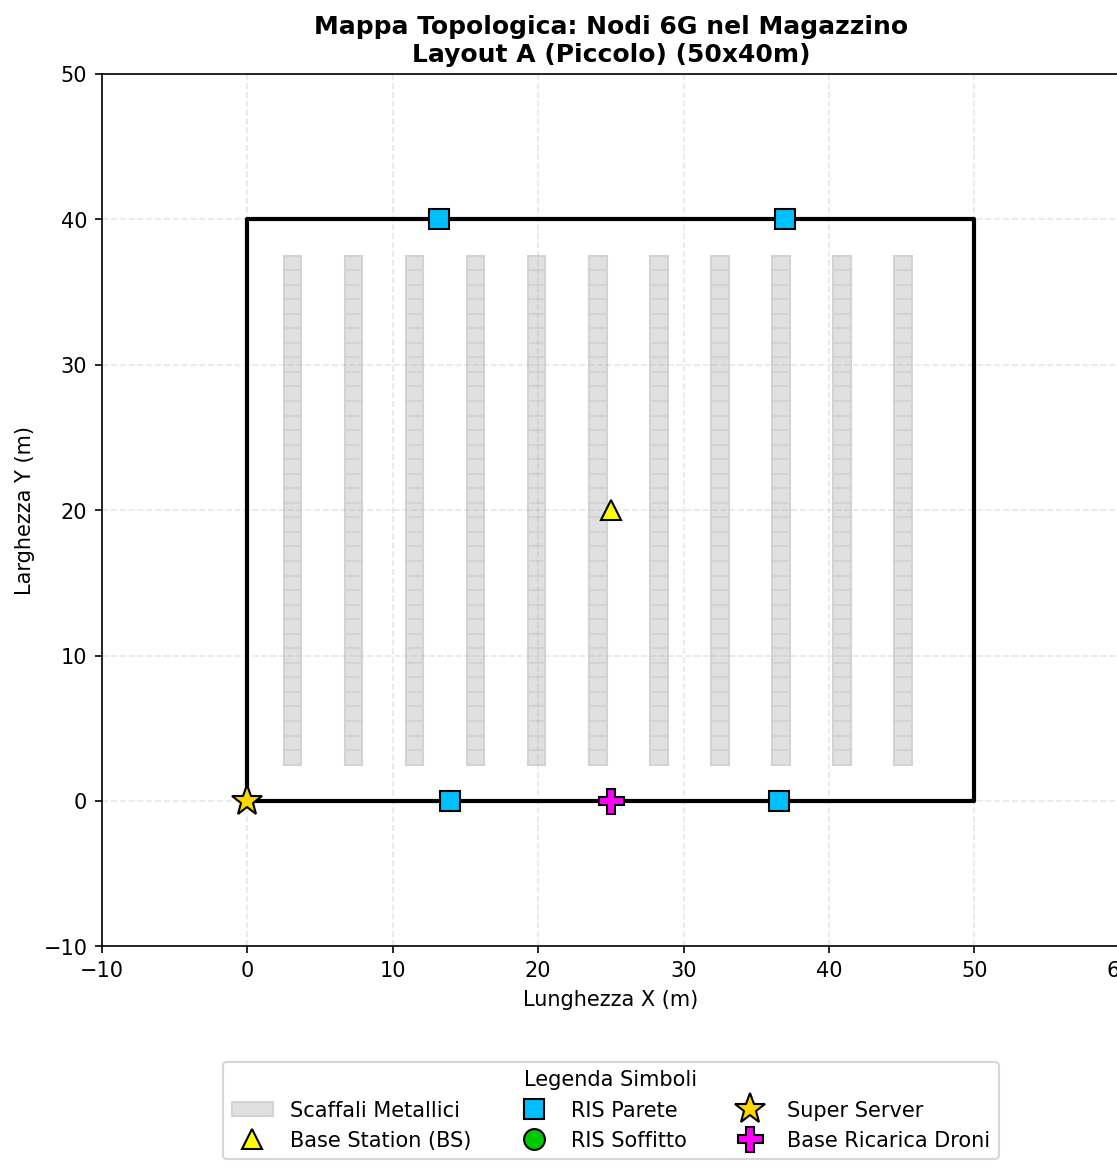
\includegraphics[width=\textwidth]{../topological_map_layout_a_nolegend.png}
        \caption{Layout A (50x40m, 4 RIS)}
    \end{subfigure}
    \hfill
    \begin{subfigure}[b]{0.48\textwidth}
        \centering
        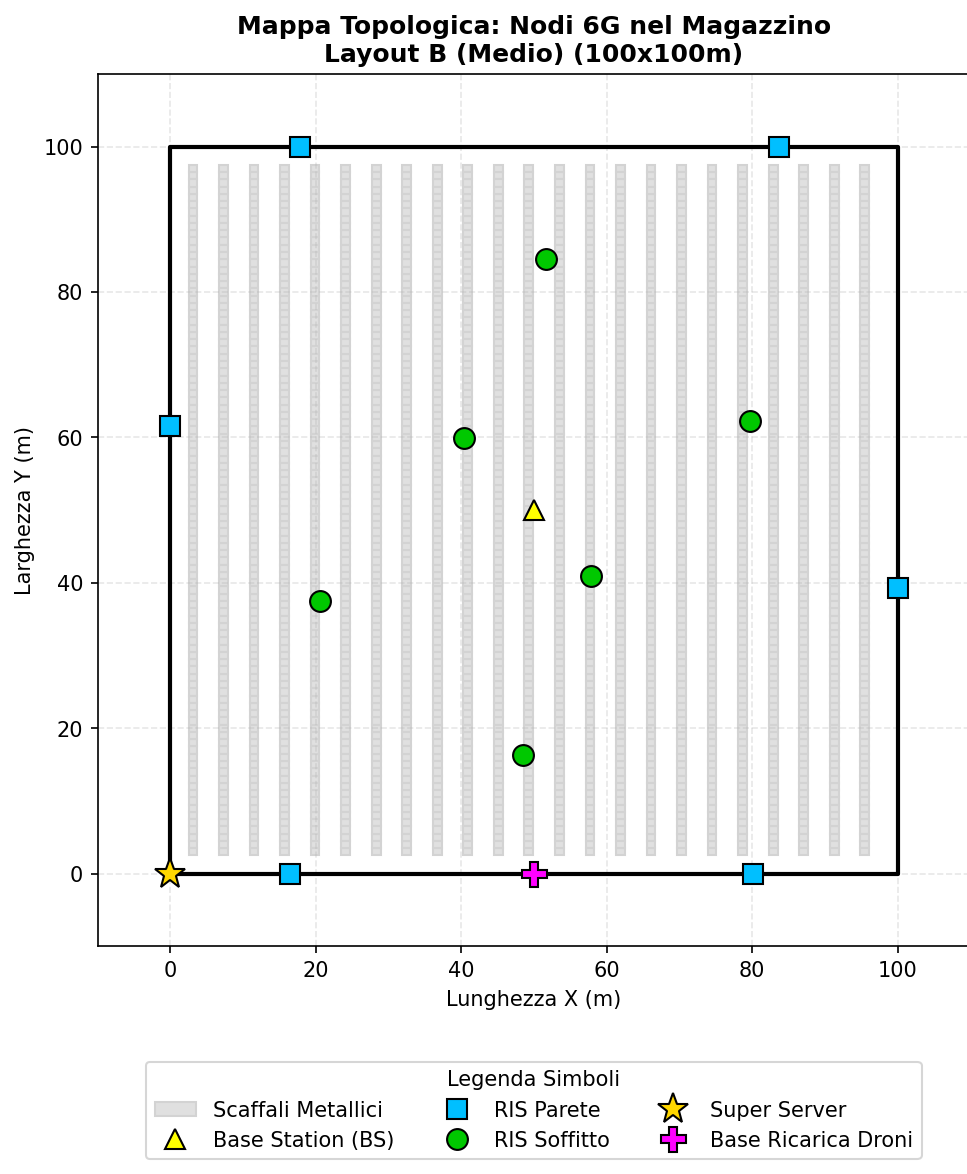
\includegraphics[width=\textwidth]{../topological_map_layout_b_nolegend.png}
        \caption{Layout B (100x100m, 12 RIS)}
    \end{subfigure}
    \caption{Mappe topologiche comparative: Scenario Piccolo (Layout A) e Standard (Layout B).}
\end{figure}

\begin{figure}[H]
    \centering
    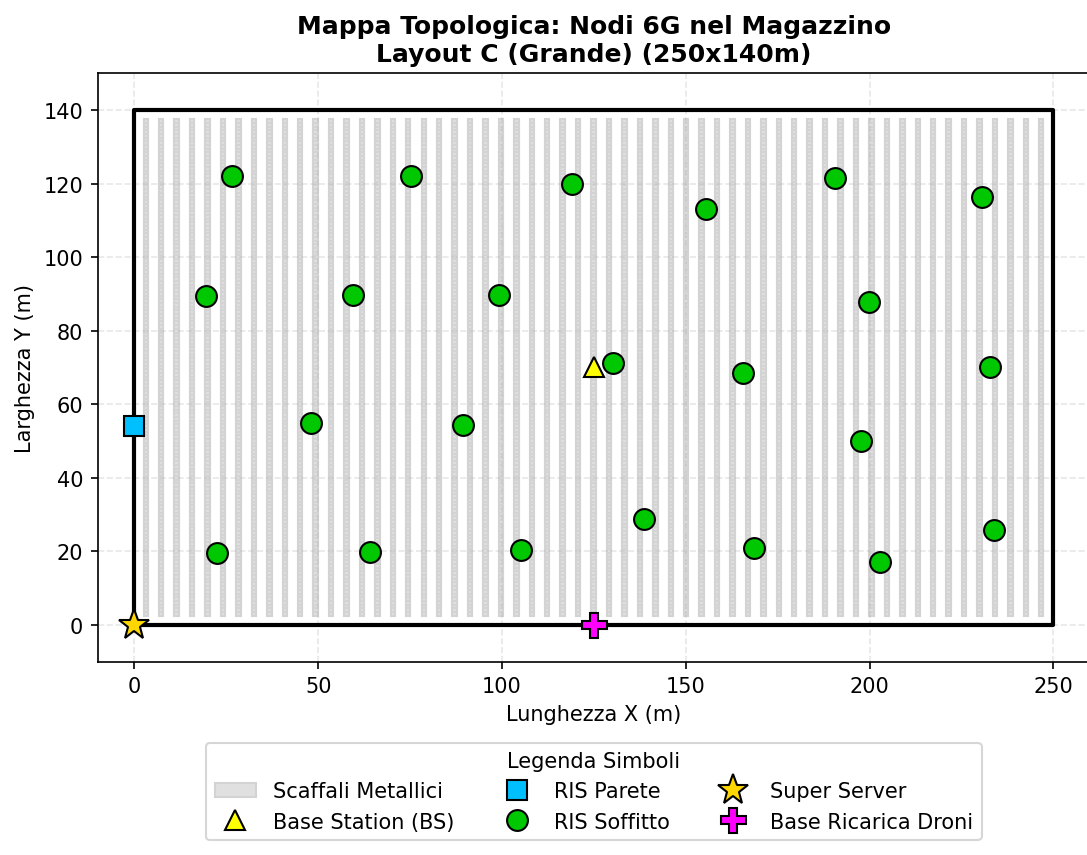
\includegraphics[width=0.6\textwidth]{../topological_map_layout_c_nolegend.png}
    \caption{Layout C VNA (250x140m, 24 RIS)}
\end{figure}

\subsubsection{I Parametri Elettromagnetici per il "6G"}
La portante di lavoro adottata per l'infrastruttura è di 5.9 GHz. Sebbene non rientri nello spettro millimetrico (mmWave/THz) prettamente target del 6G, costituisce attulamente lo standard consolidato nel panorama C-V2X (\textit{Cellular Vehicle-to-Everything}) per le reti \textit{mission-critical} veicolari.
Il \textit{front-end} ricevente è stato modellato con una stringente soglia di sensibilità: qualora il \textit{Signal-to-Noise Ratio} (SNR) scenda sotto il limite di 5 dB, i campioni vengono scartati e si certifica l'ingresso in \textit{Outage Zone} radiopropagativa. 
Inerentemente all'assorbimento termodinamico delle RIS, i modelli di rete riflettono curve fisicamente verosimili: uno stato \textit{idle} o passivo a ridottissima dissipazione (0.5 W), ed una transizione \textit{active} deputata al \textit{beamforming}, il cui consumo converge attorno ai 50 W, garantendo parallelamente un guadagno d'antenna stimato prossimo ai +20 dB.

\subsubsection{Il Drone e il Cervello Matematico (Filtro EKF)}
Il sistema aeromobile a pilotaggio remoto simulato (UAV) rispecchia le dinamiche cinematiche di un quadrirotore merci leggero operativo, avente modulo della velocità vettoriale pari a circa 3.0 m/s in moto rettilineo uniforme. 
Il nucleo del tracciamento indoor risiede nell'implementazione dell'Extended Kalman Filter (EKF). Il filtro statuale operante ad una frequenza di aggiornamento di 10 Hz attua la data fusion tra le equazioni differenziali del moto e le rilevazioni sensoristiche telemetriche dell'SDN. Risulta imperativo notare che, a fronte di interruzioni prolungate delle letture esterne dovute ad attenuazioni gravose (il regime NLoS e conseguente \textit{Outage} dei sensori lineari), il filtro diviene inservibile sul fronte dei residui di misura e si sbilancia forzatamente verso le sole matrici predittive basate sull'ultima stima cinematica conosciuta (\textit{navigazione inerziale pura}).

\newpage
\subsection{Test 1: Analisi Baseline NLoS e fallimento del tracciamento (Diagnosi)}

Allo scopo di validare le dipendenze critiche dall'infrastruttura di supporto, il Test 1 delinea la condizione di \textit{baseline}, analizzando la performance del tracking EKF in assenza totale di superfici riflettenti. Per tale modulo, il collaudo prevede profili di volo articolati che costringono l'UAV ad alternare transizioni repentine tra segmenti prettamente in Line-of-Sight (LoS) e prolungate latitanze in refrattivi complessi a morfologia Non-Line-of-Sight (NLoS).

\subsubsection{Decadimento del Link Radio e Transizione in "Coasting" Inerziale}
Dal punto di vista della simulazione al calcolatore, la compromissione radiopropagativa è gestita dal motore basato su \textit{ray-casting}. Non appena il velivolo oltrepassa la linea ortogonale dello scaffale, le densità ostacolanti erigono immediate sfavorevoli condizioni fisiche che conducono ai limiti inaccettabili dell'attenuazione. Il simulatore calcola un rapido incremento di \textit{Path Loss} che fa collassare il segnale-rumore (SNR) sotto la soglia di demarcazione dei 5 dB.
In risposta immediata a tale carenza deterministica, il modulo software dell'\textbf{Extended Kalman Filter (EKF)}, privato delle misurazioni di distanza \textit{Time-of-Flight}, disabilita la correzione ponderata derivante dai residui (fase di Update) e commuta automaticamente nel loop \textit{open-course} denominato comunemente modalità \textbf{"Coasting"}. In questo stato, le stime del vettore continuano basandosi pedissequamente sulle leggi matriciali di moto lineare ipotizzando l'assenza di ulteriori perturbazioni dinamiche.

\subsubsection{Deriva della Stima Spaziale e Saturazione delle Covarianze}
L'osservazione topologica estratta in output per layout a complessità media ed elevata (Layout B e C) evidenzia severe distorsioni geometriche causate dal blocco della doppia integrazione del rumore inerziale:

\begin{enumerate}
    \item \textbf{Drift Metrico Cumulativo (Divergenza Spaziale):} Nelle viste \textit{Top-Down}, si evidenzia la rigorosa sovrapposizione iniziale della predizione EKF (traccia tratteggiata rossa) con la traiettoria di simulazione reale del \textit{Ground Truth} (verde). Tale corrispondenza collassa integralmente all'accesso in regione NLoS profonda: la distanza d'errore si amplifica monotonamente conducendo il tracciamento terminale in disallineamenti di svariati metri. 
    \item \textbf{Crescita Monotona della Traccia della Matrice di Covarianza (P):} A confermare la solidità dell'implementazione computazionale, è possibile osservare l'espansione spaziale delle ellissi probabilistiche attestanti l'errore gaussiano dell'UAV. Ogni ciclo d'estimo carente di stima radio inietta incertezza cumulabile.
\end{enumerate}

\begin{figure}[H]
    \centering
    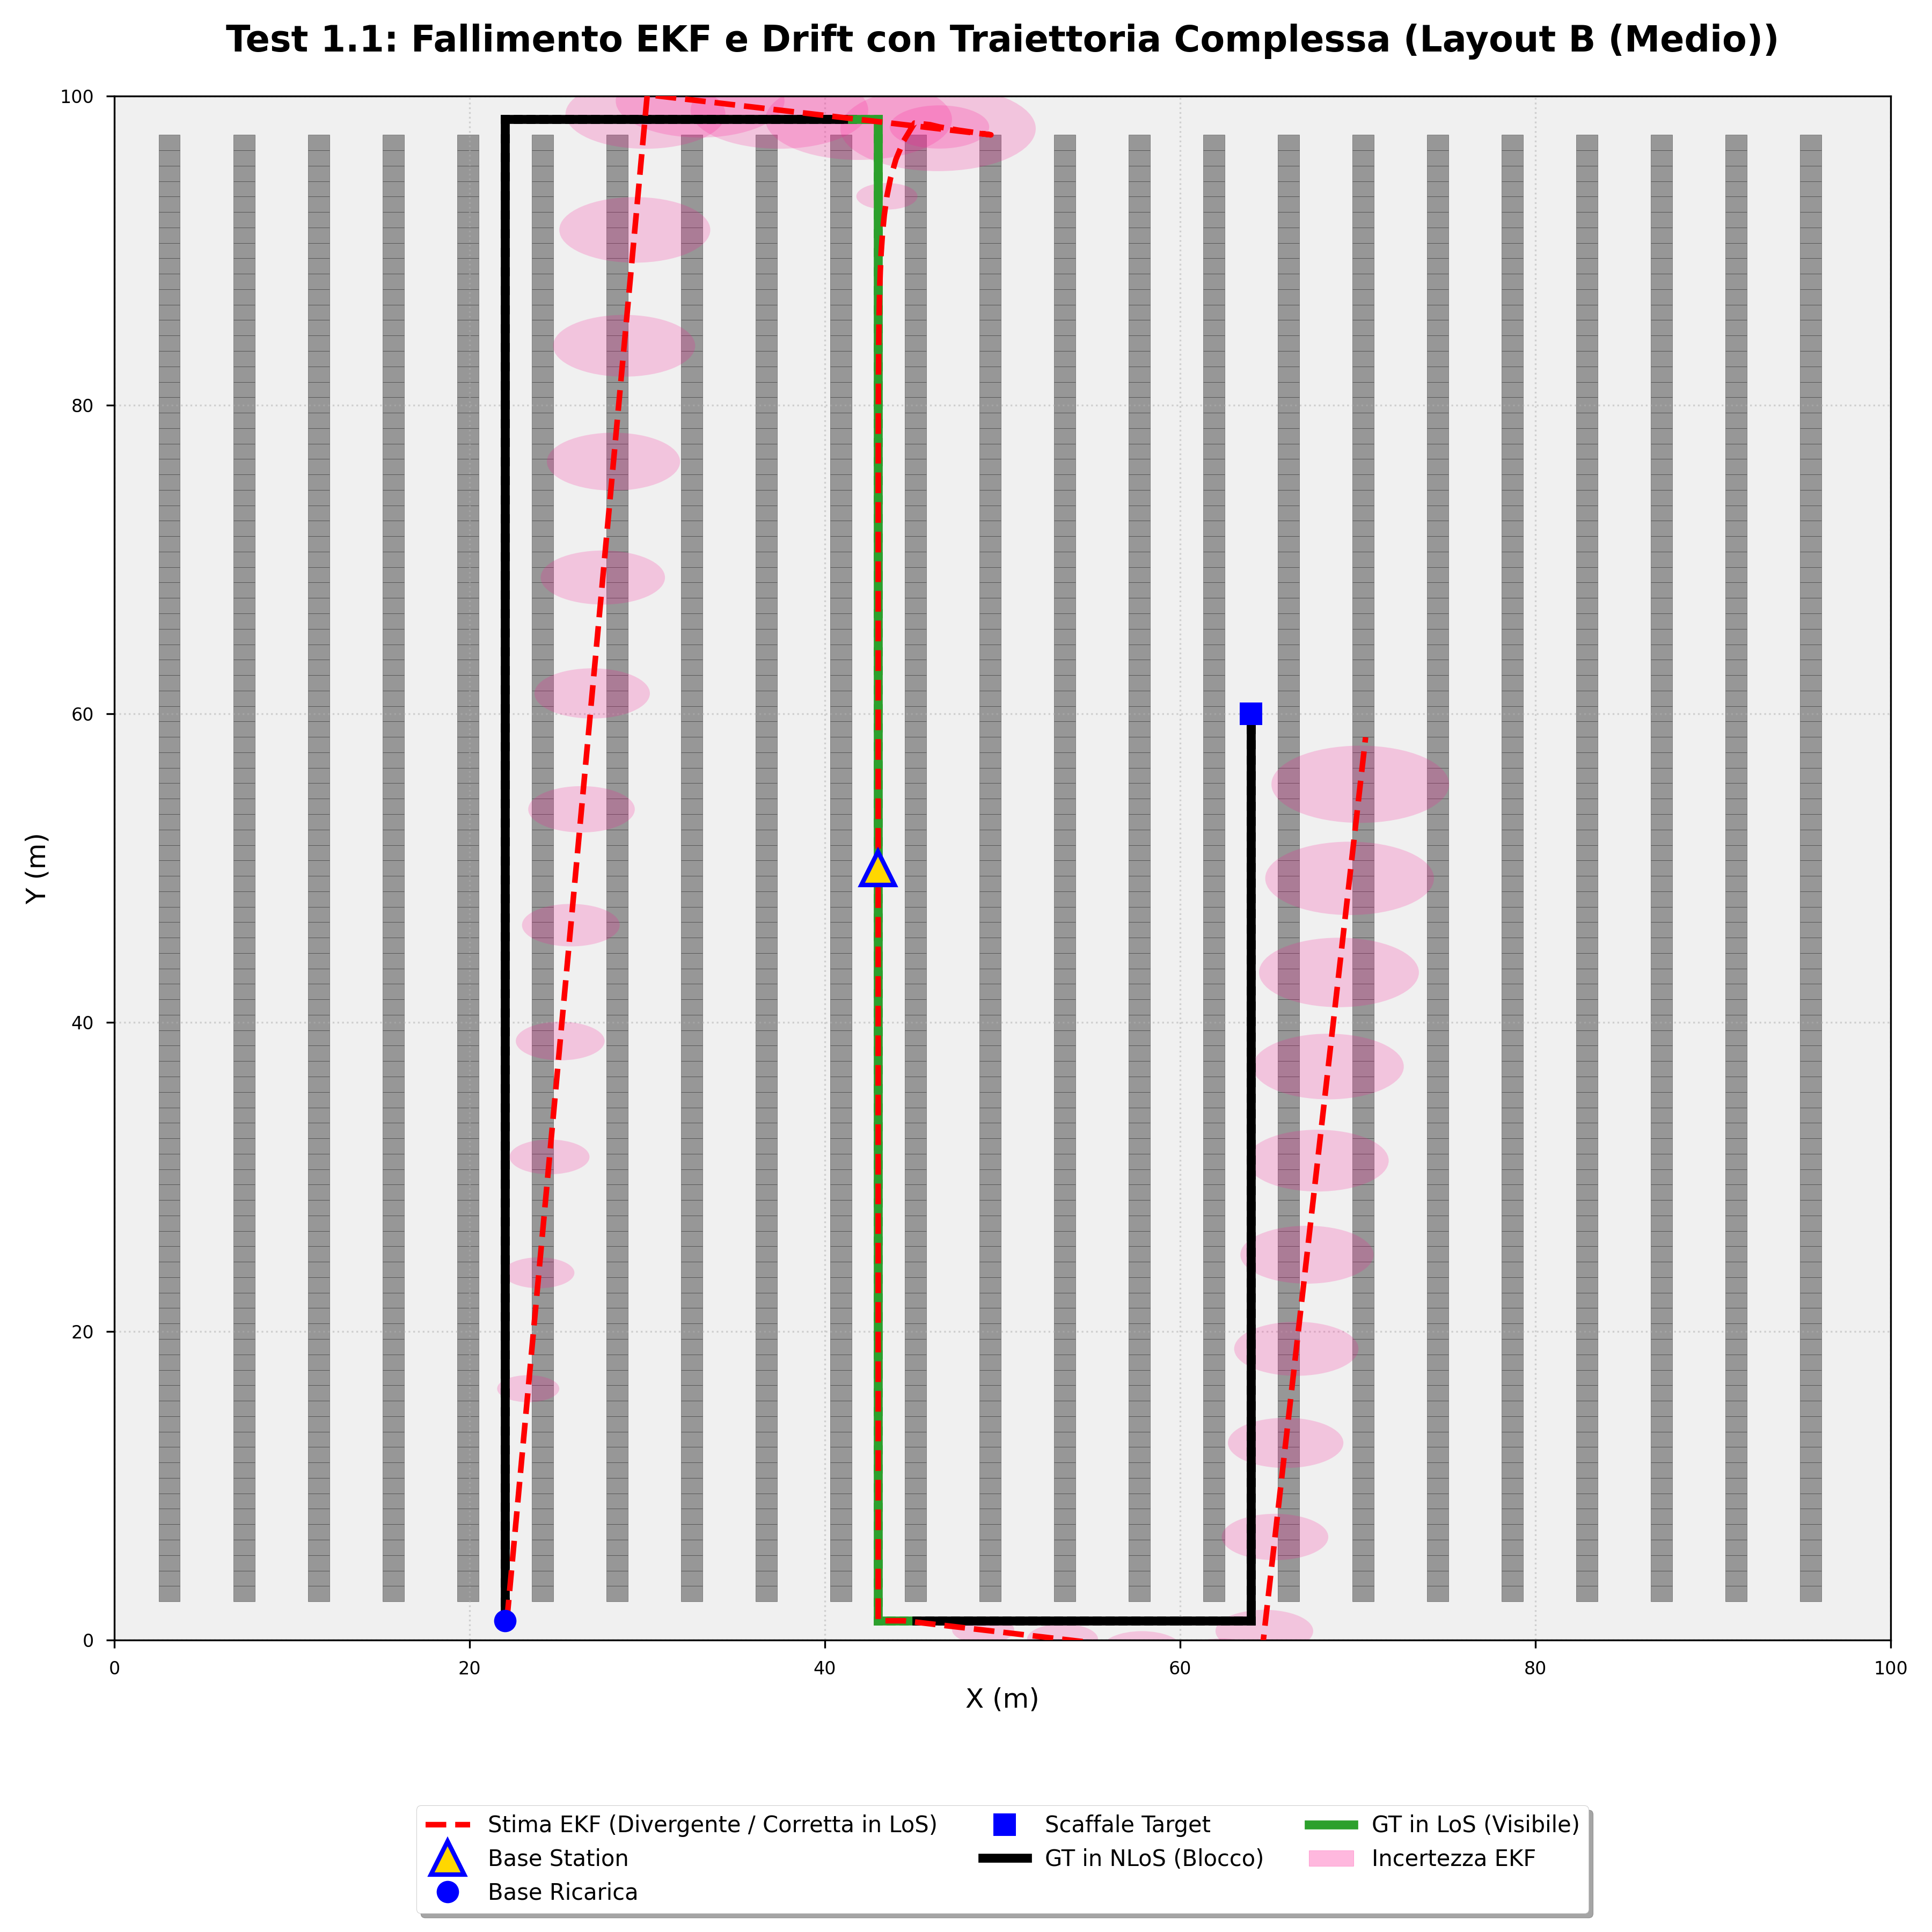
\includegraphics[width=0.65\textwidth]{../Test_1_B_TopDown_Traiettoria.png}
    \caption{Test 1 (Layout B). Divergenza della traiettoria stimata dall'EKF e logica Coasting.}
    \label{fig:test1_traiettoria}
\end{figure}


\subsubsection{Analisi Quantitativa: Root Mean Square Error e Distribuzione Cumulativa}
Ad integrazione dell'analisi fenomenologico-spaziale, gli algoritmi di back-end del simulatore hanno campionato la norma degli scarti producendo il grafico dell'errore quadratico medio temporale (RMSE) nonché la rispettiva stima di densità probabilistica cumulativa (CDF). L'analisi riscontra incontrovertibilmente il degrado prestazionale transitorio in NLoS.

\begin{figure}[H]
    \centering
    \begin{subfigure}[b]{0.48\textwidth}
        \centering
        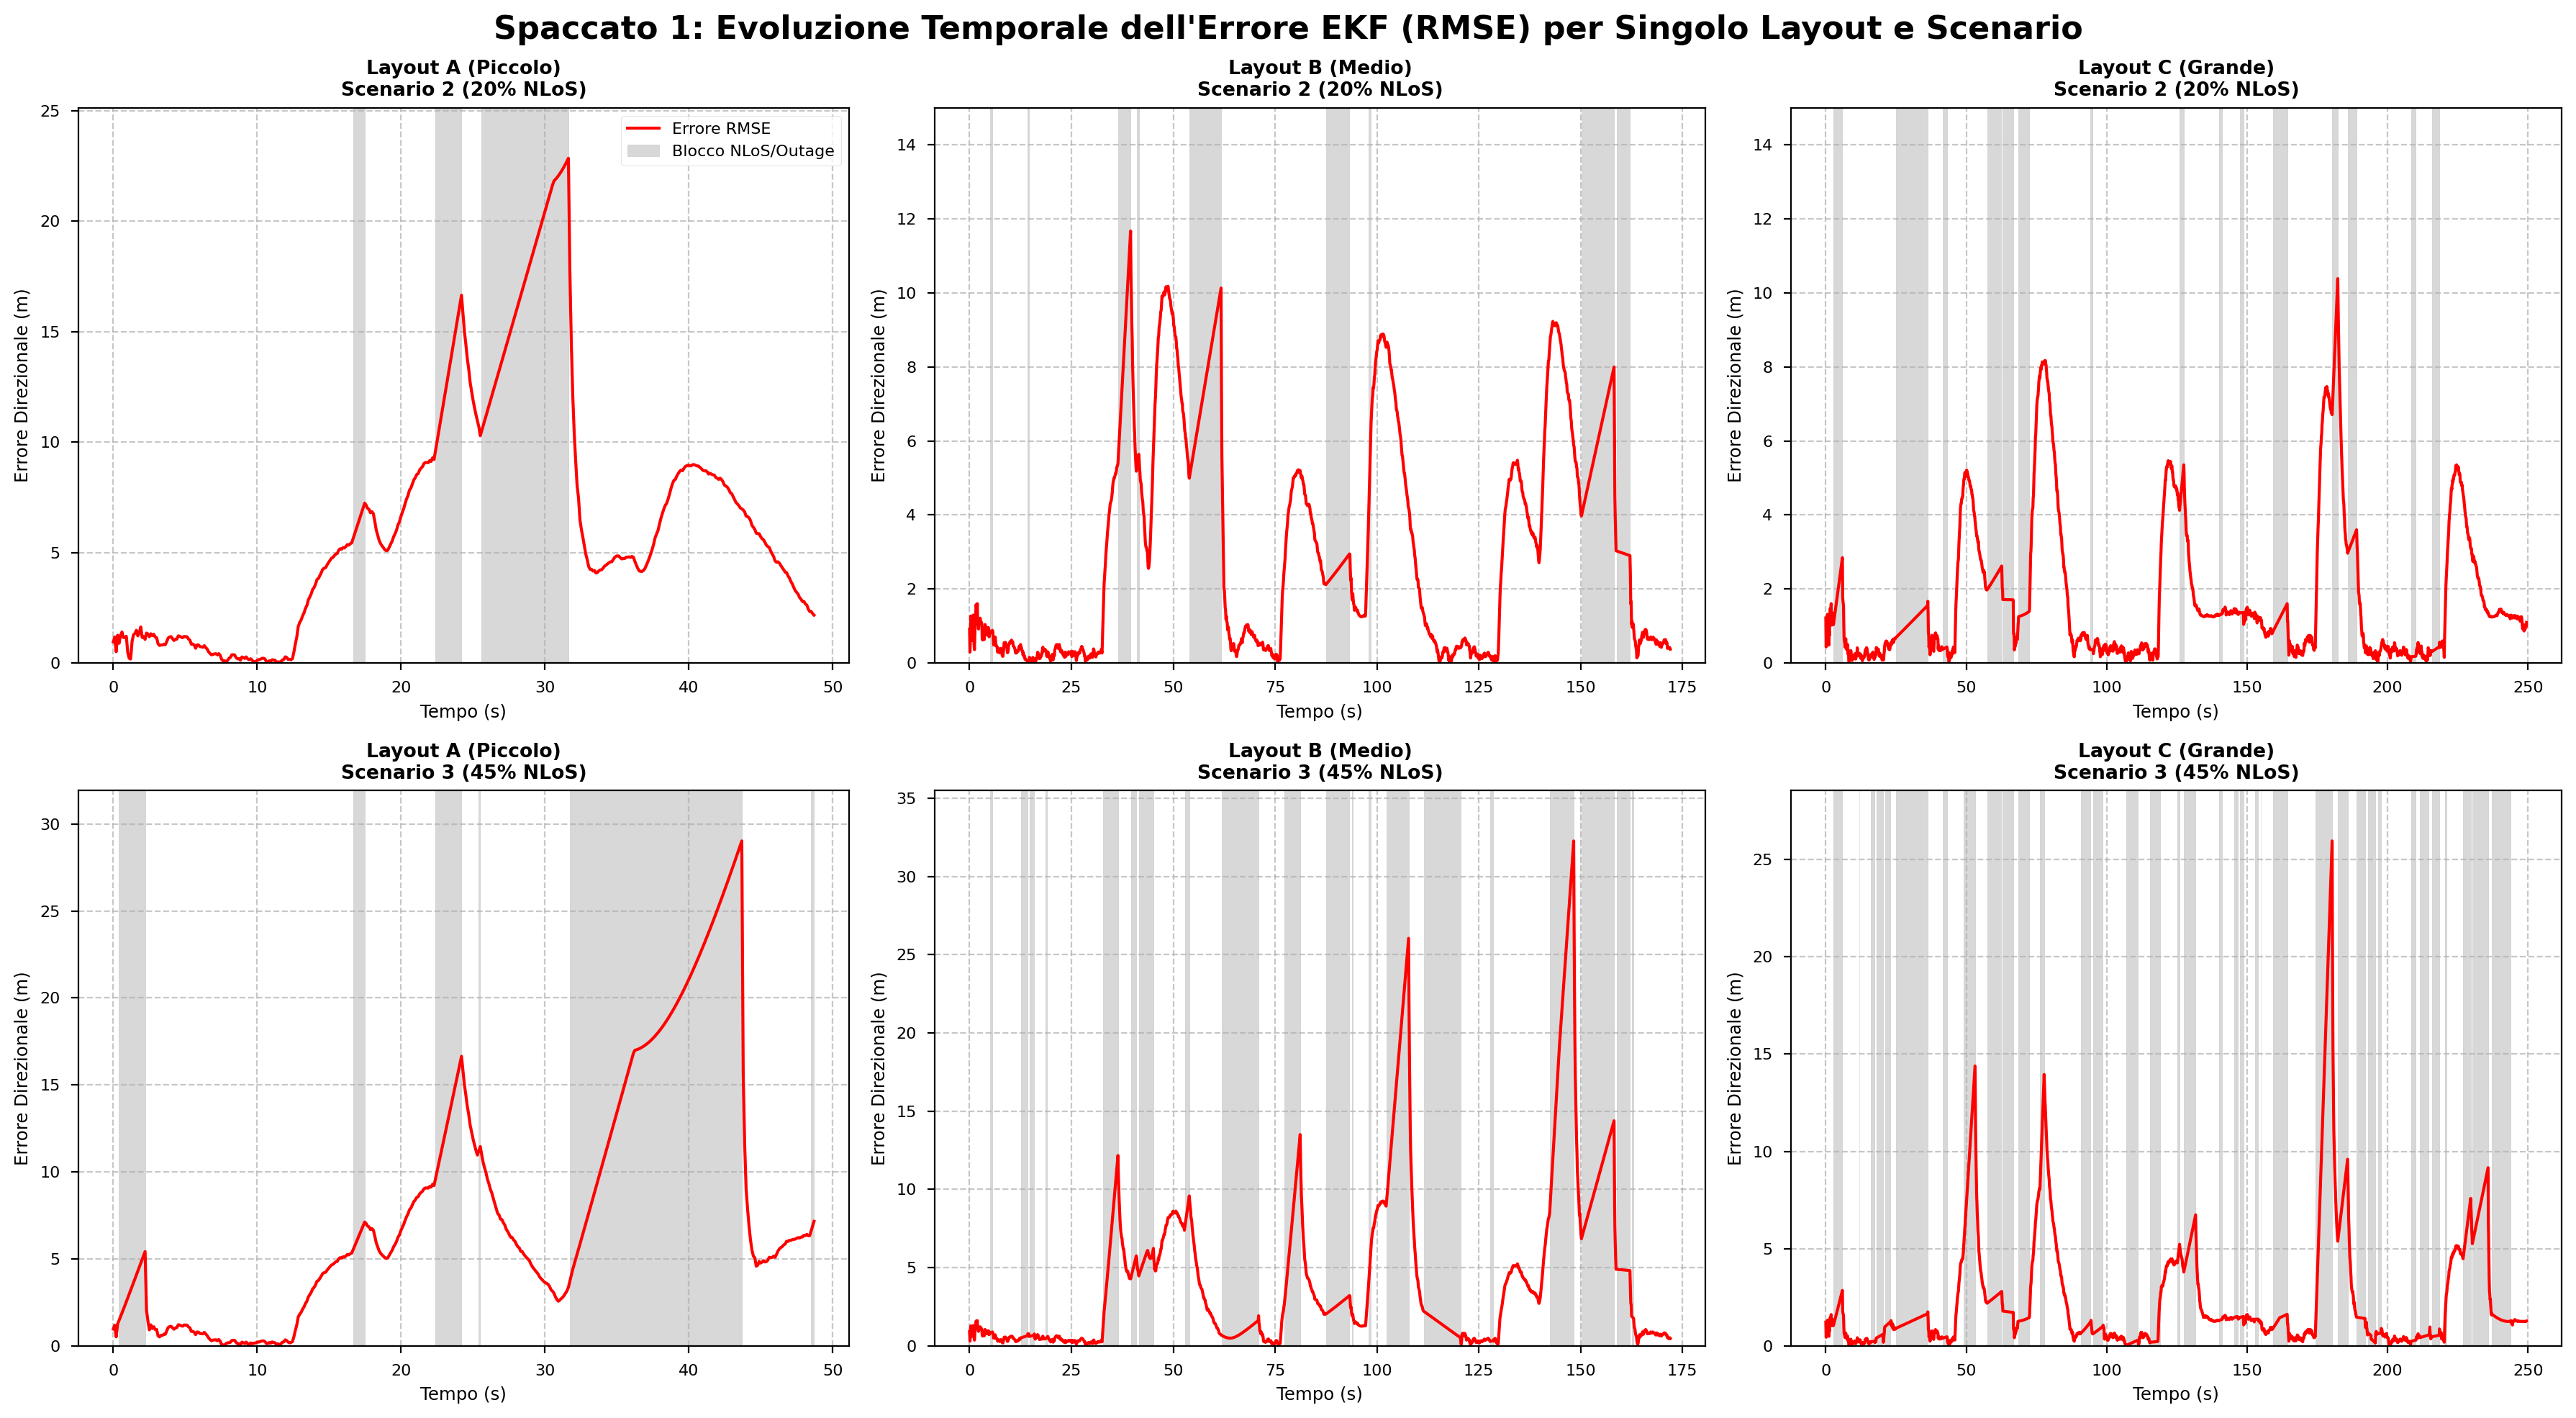
\includegraphics[width=\textwidth]{../Test_1_RMSE_Temporale.png}
        \caption{Curva Tempo RMSE}
    \end{subfigure}
    \hfill
    \begin{subfigure}[b]{0.48\textwidth}
        \centering
        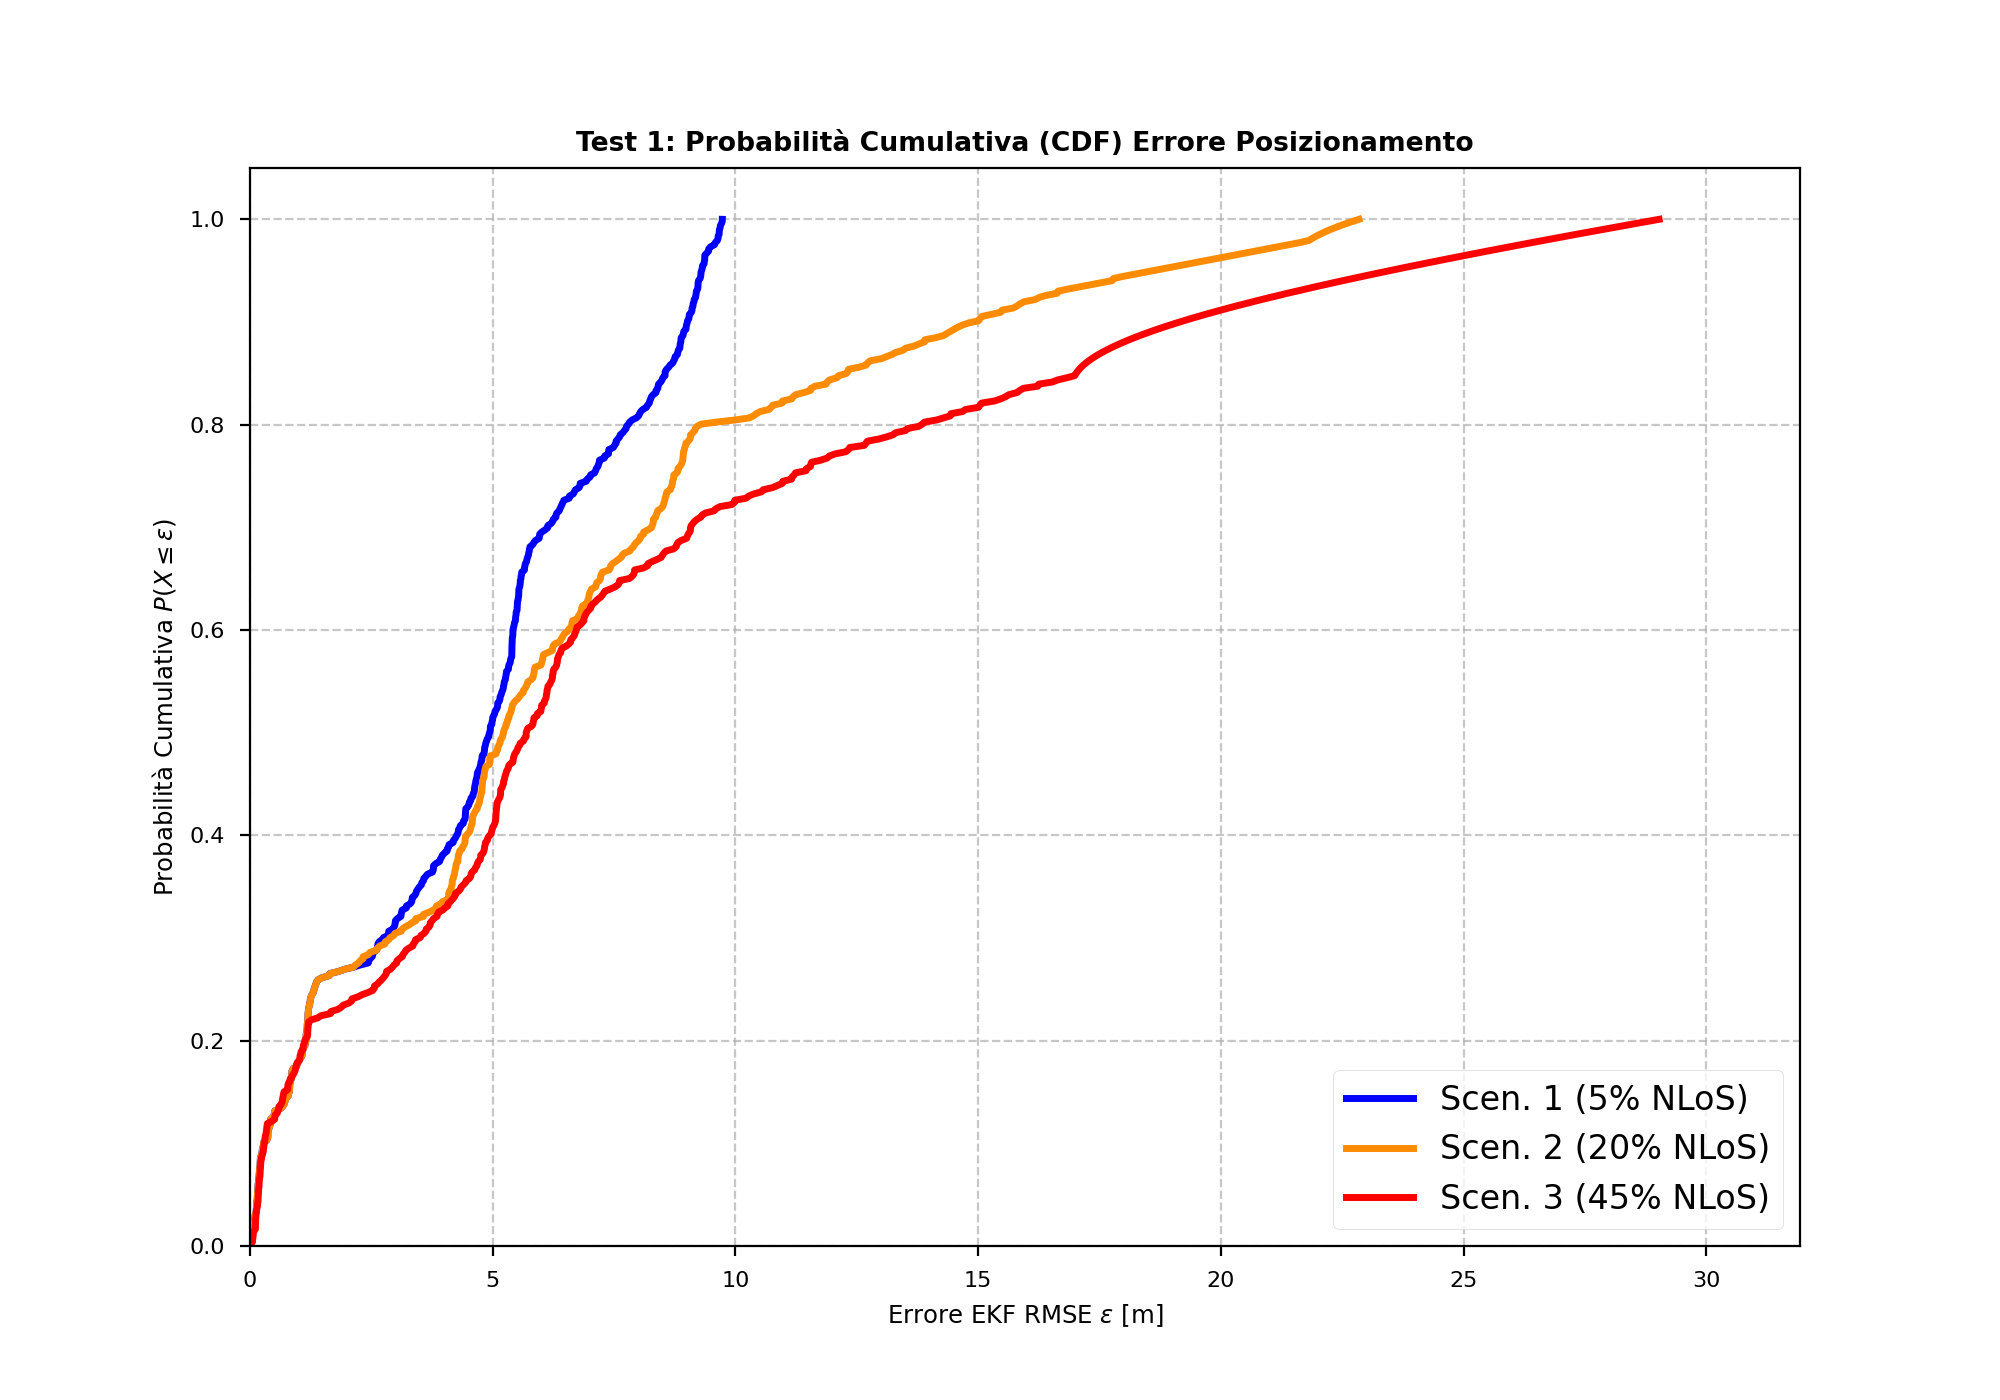
\includegraphics[width=\textwidth]{../Test_1_CDF_RMSE.png}
        \caption{CDF RMSE}
    \end{subfigure}
    \caption{Test 1: Decadimento metrico dell'errore spaziale in NLoS puro.}
    \label{fig:test1_rmse}
\end{figure}

\subsection{Test 2: Mitigazione degli Scenari NLoS tramite Assisted-Line-of-Sight}

Constatate le vulnerabilità inerziali del tracciamento standard, la seconda fase sperimentale ha visto attivato l'agente orchestratore globale (livello SDN). La rete possiede l'autorizzazione all'ingaggio attivo degli specchi intelligenti pre-allocati, procedendo nell'inoltro del campo elettromagnetico e nell'incremento sostanziale della potenza irraggiata verso il veicolo bersaglio coperto.

\subsubsection{Ripristino Analogico: Assisted-Line-of-Sight}
Il costrutto logico su cui insiste l'architettura si articola come segue: l'intelligenza SDN, in virtù dei propri profili di visibilità topologica, conosce l'allocazione degli ostacoli in riferimento all'attuale \textit{heading} dell'UAV. Nell'istante esatto di penetramento dell'angolatura di deflessione NLoS, la centralina invia una retta direttiva al nodo RIS ottimale sulla rispettiva parete visibile.
Tale direttiva demanda alla RIS di calibrare un protocollo di correzione di propagazione di fase per direzionare e focalizzare i multi-cammini all'ingresso del corridoio. Questo processo computazionale concretizza in letteratura la cosiddetta \textbf{Assisted-Line-of-Sight} (Linea di Vista Assistita, A-LoS). Ne consegue un transitorio ripristino della densità di segnale, che supera abbondantemente la soglia fisica dei 5 dB di cutoff dell'antenna, mitigando in sicurezza il blocco radiopropagativo preesistente.

\subsubsection{Rientro a Pieno Regime EKF della Stima Metrica}
\begin{figure}[H]
    \centering
    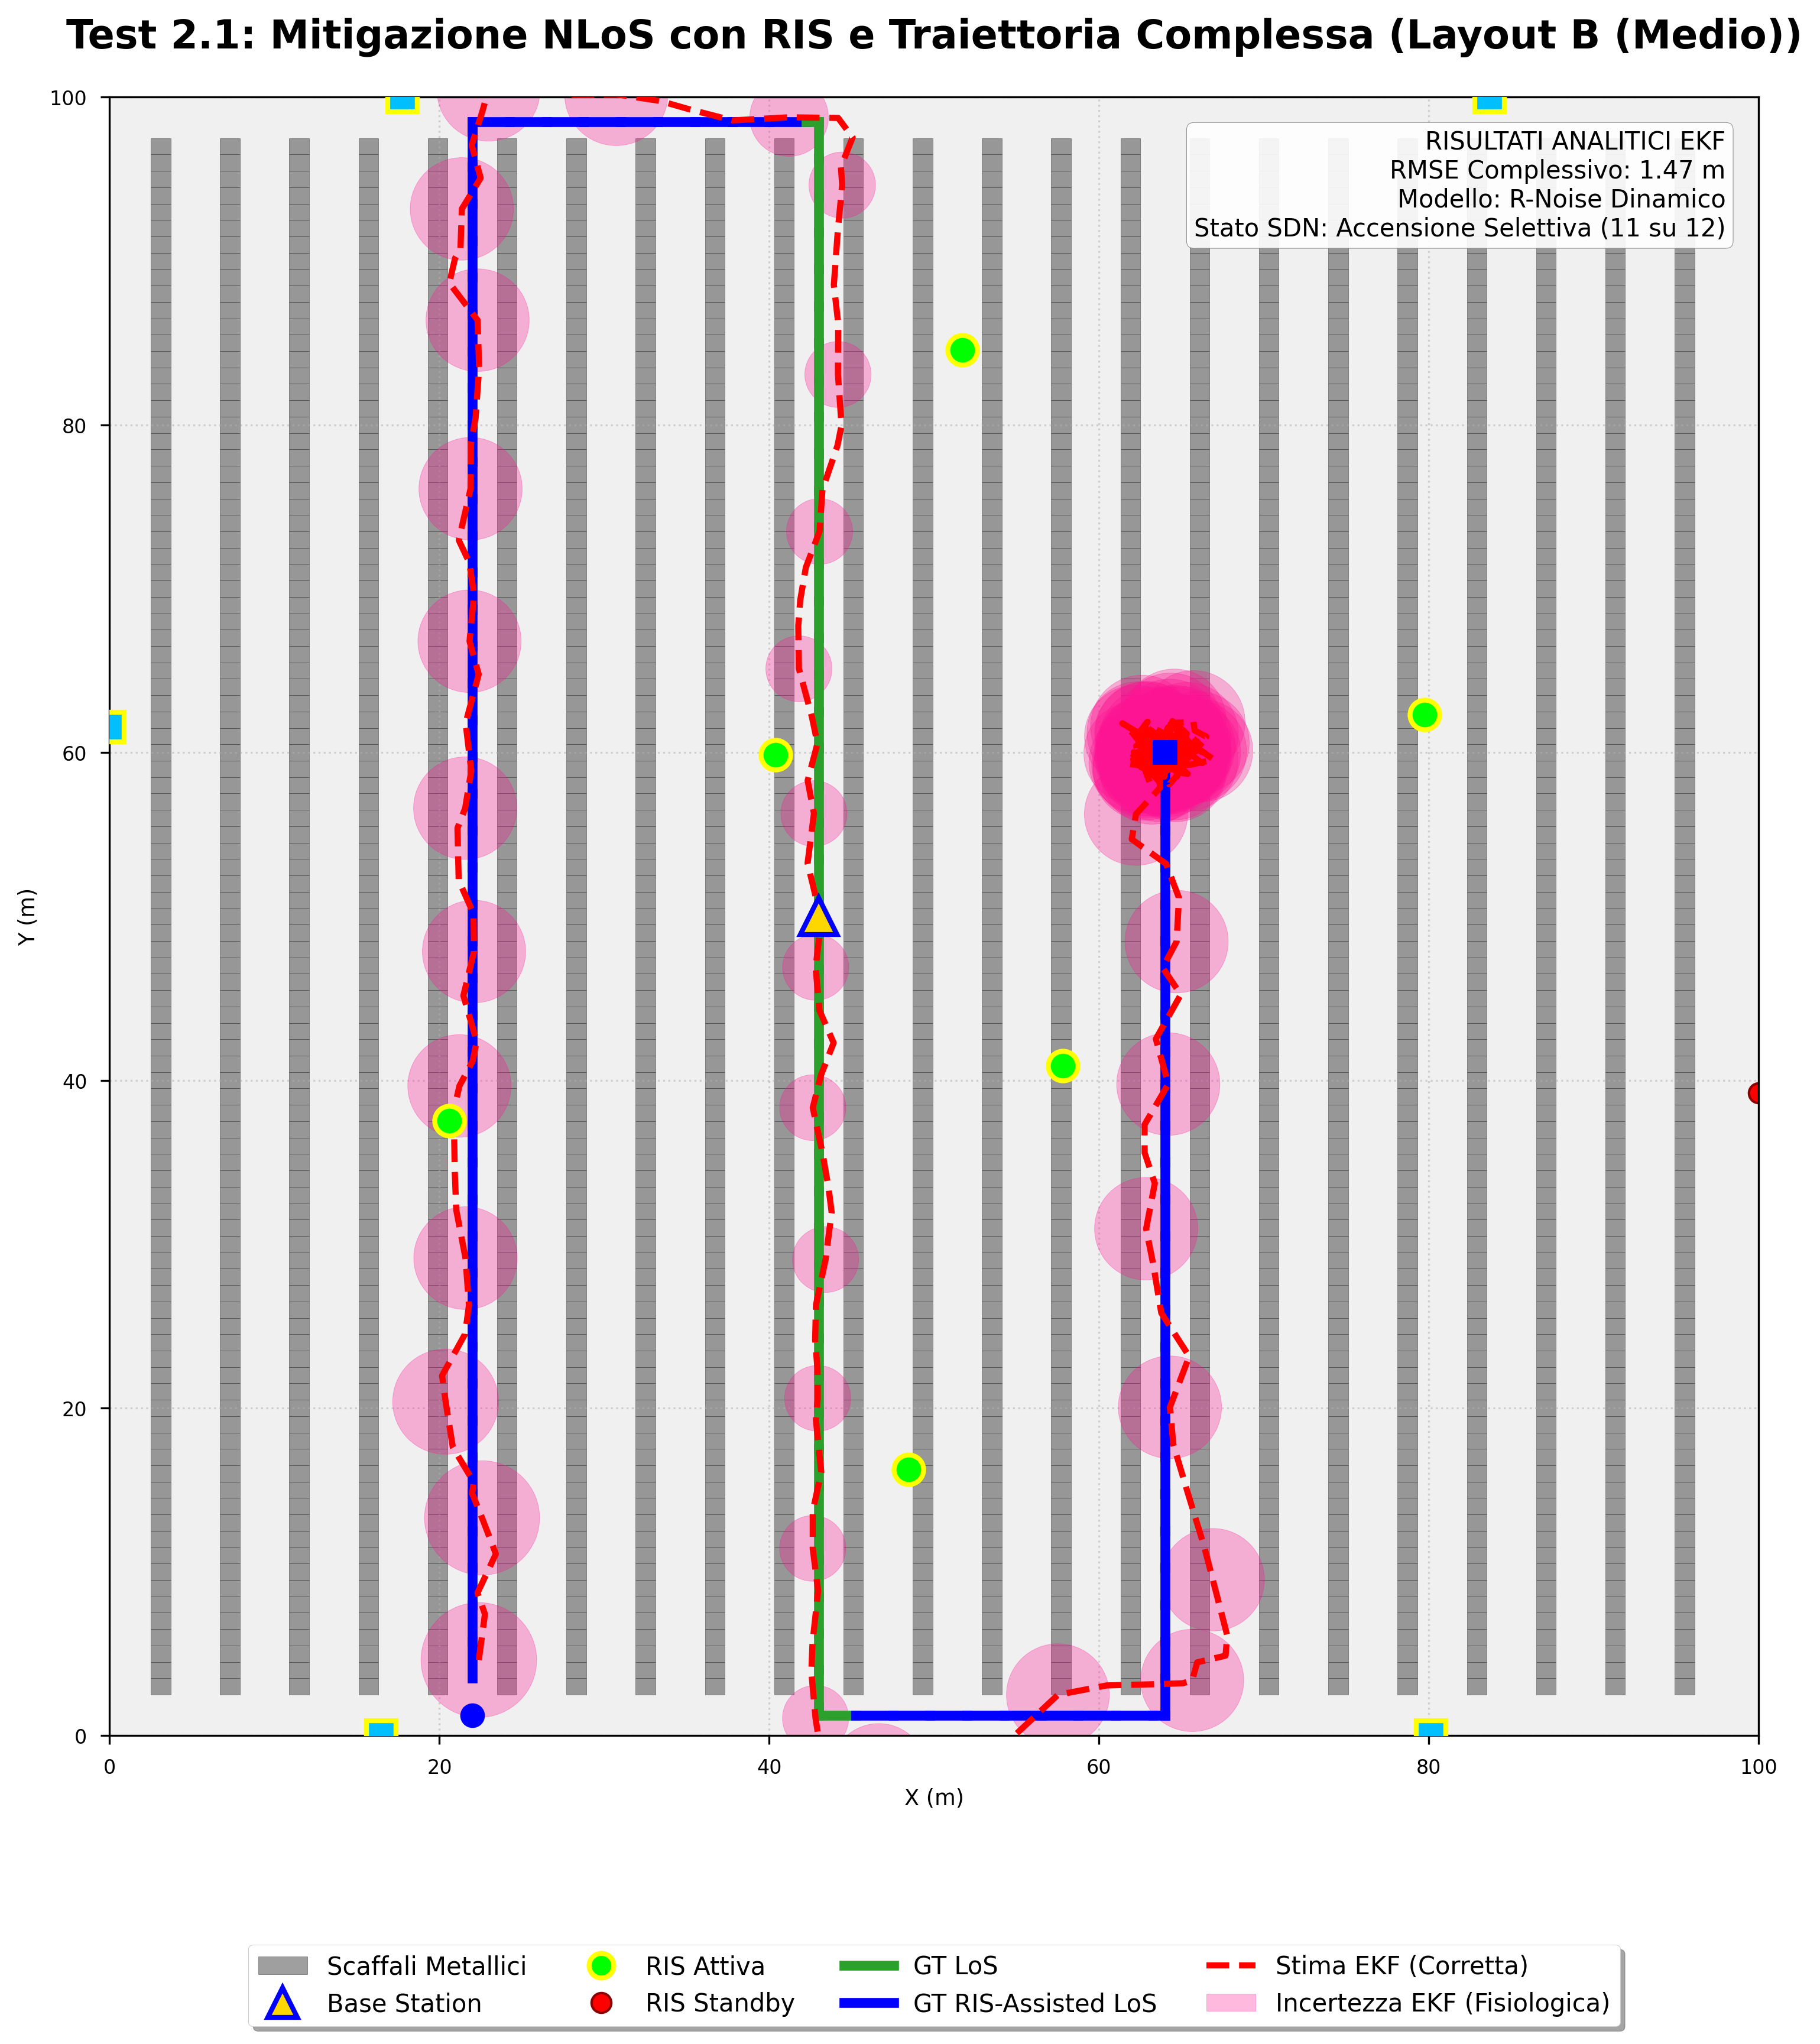
\includegraphics[width=0.6\textwidth]{../Test_2_B_Successo_RIS.png}
    \caption{Test 2: Con la RIS attiva per A-LoS interviene il ripristino EKF metrico.}
    \label{fig:test2_successo}
\end{figure}

I risultati conseguiti a fronte delle simulazioni del Test 2 convalidano l'efficienza del modello strutturato preposto.
L'azione compensativa della logica RIS reintegra il loop operazionale di aggiornamento (\textit{Innovation Step}) nel ciclo discreto del filtro EKF, interrompendone e correggendone la vertiginosa crescita d'errore autonomo sperimentato nel Test 1.
In chiave analitica quantitativa, si registra la correzione subitanea degli scarti quadratici transitori, il cui modulo geometrico si stabilisce saldamente e permanentemente nel perimetro del raggio di circa \textbf{1.0 m}. Considerate le imperfezioni multi-cammino e l'elevata trazione cinetica di un drone (3 m/s) tra pareti di metallo, questo parametro risulta ampiamente appianante e validante le normative di \textit{safety}.
Al contempo, sul piano spaziale-probabilistico di covarianza (rif. Figura \ref{fig:test2_rmse}) si certifica l'efficacia algoritmica di re-contrazione della matrice d'incertezza $P$: l'enorme alone ellittico si svuota quasi istantaneamente riattorno ai baricentri reali fisici operanti.



\begin{figure}[H]
    \centering
    \begin{subfigure}[b]{0.48\textwidth}
        \centering
        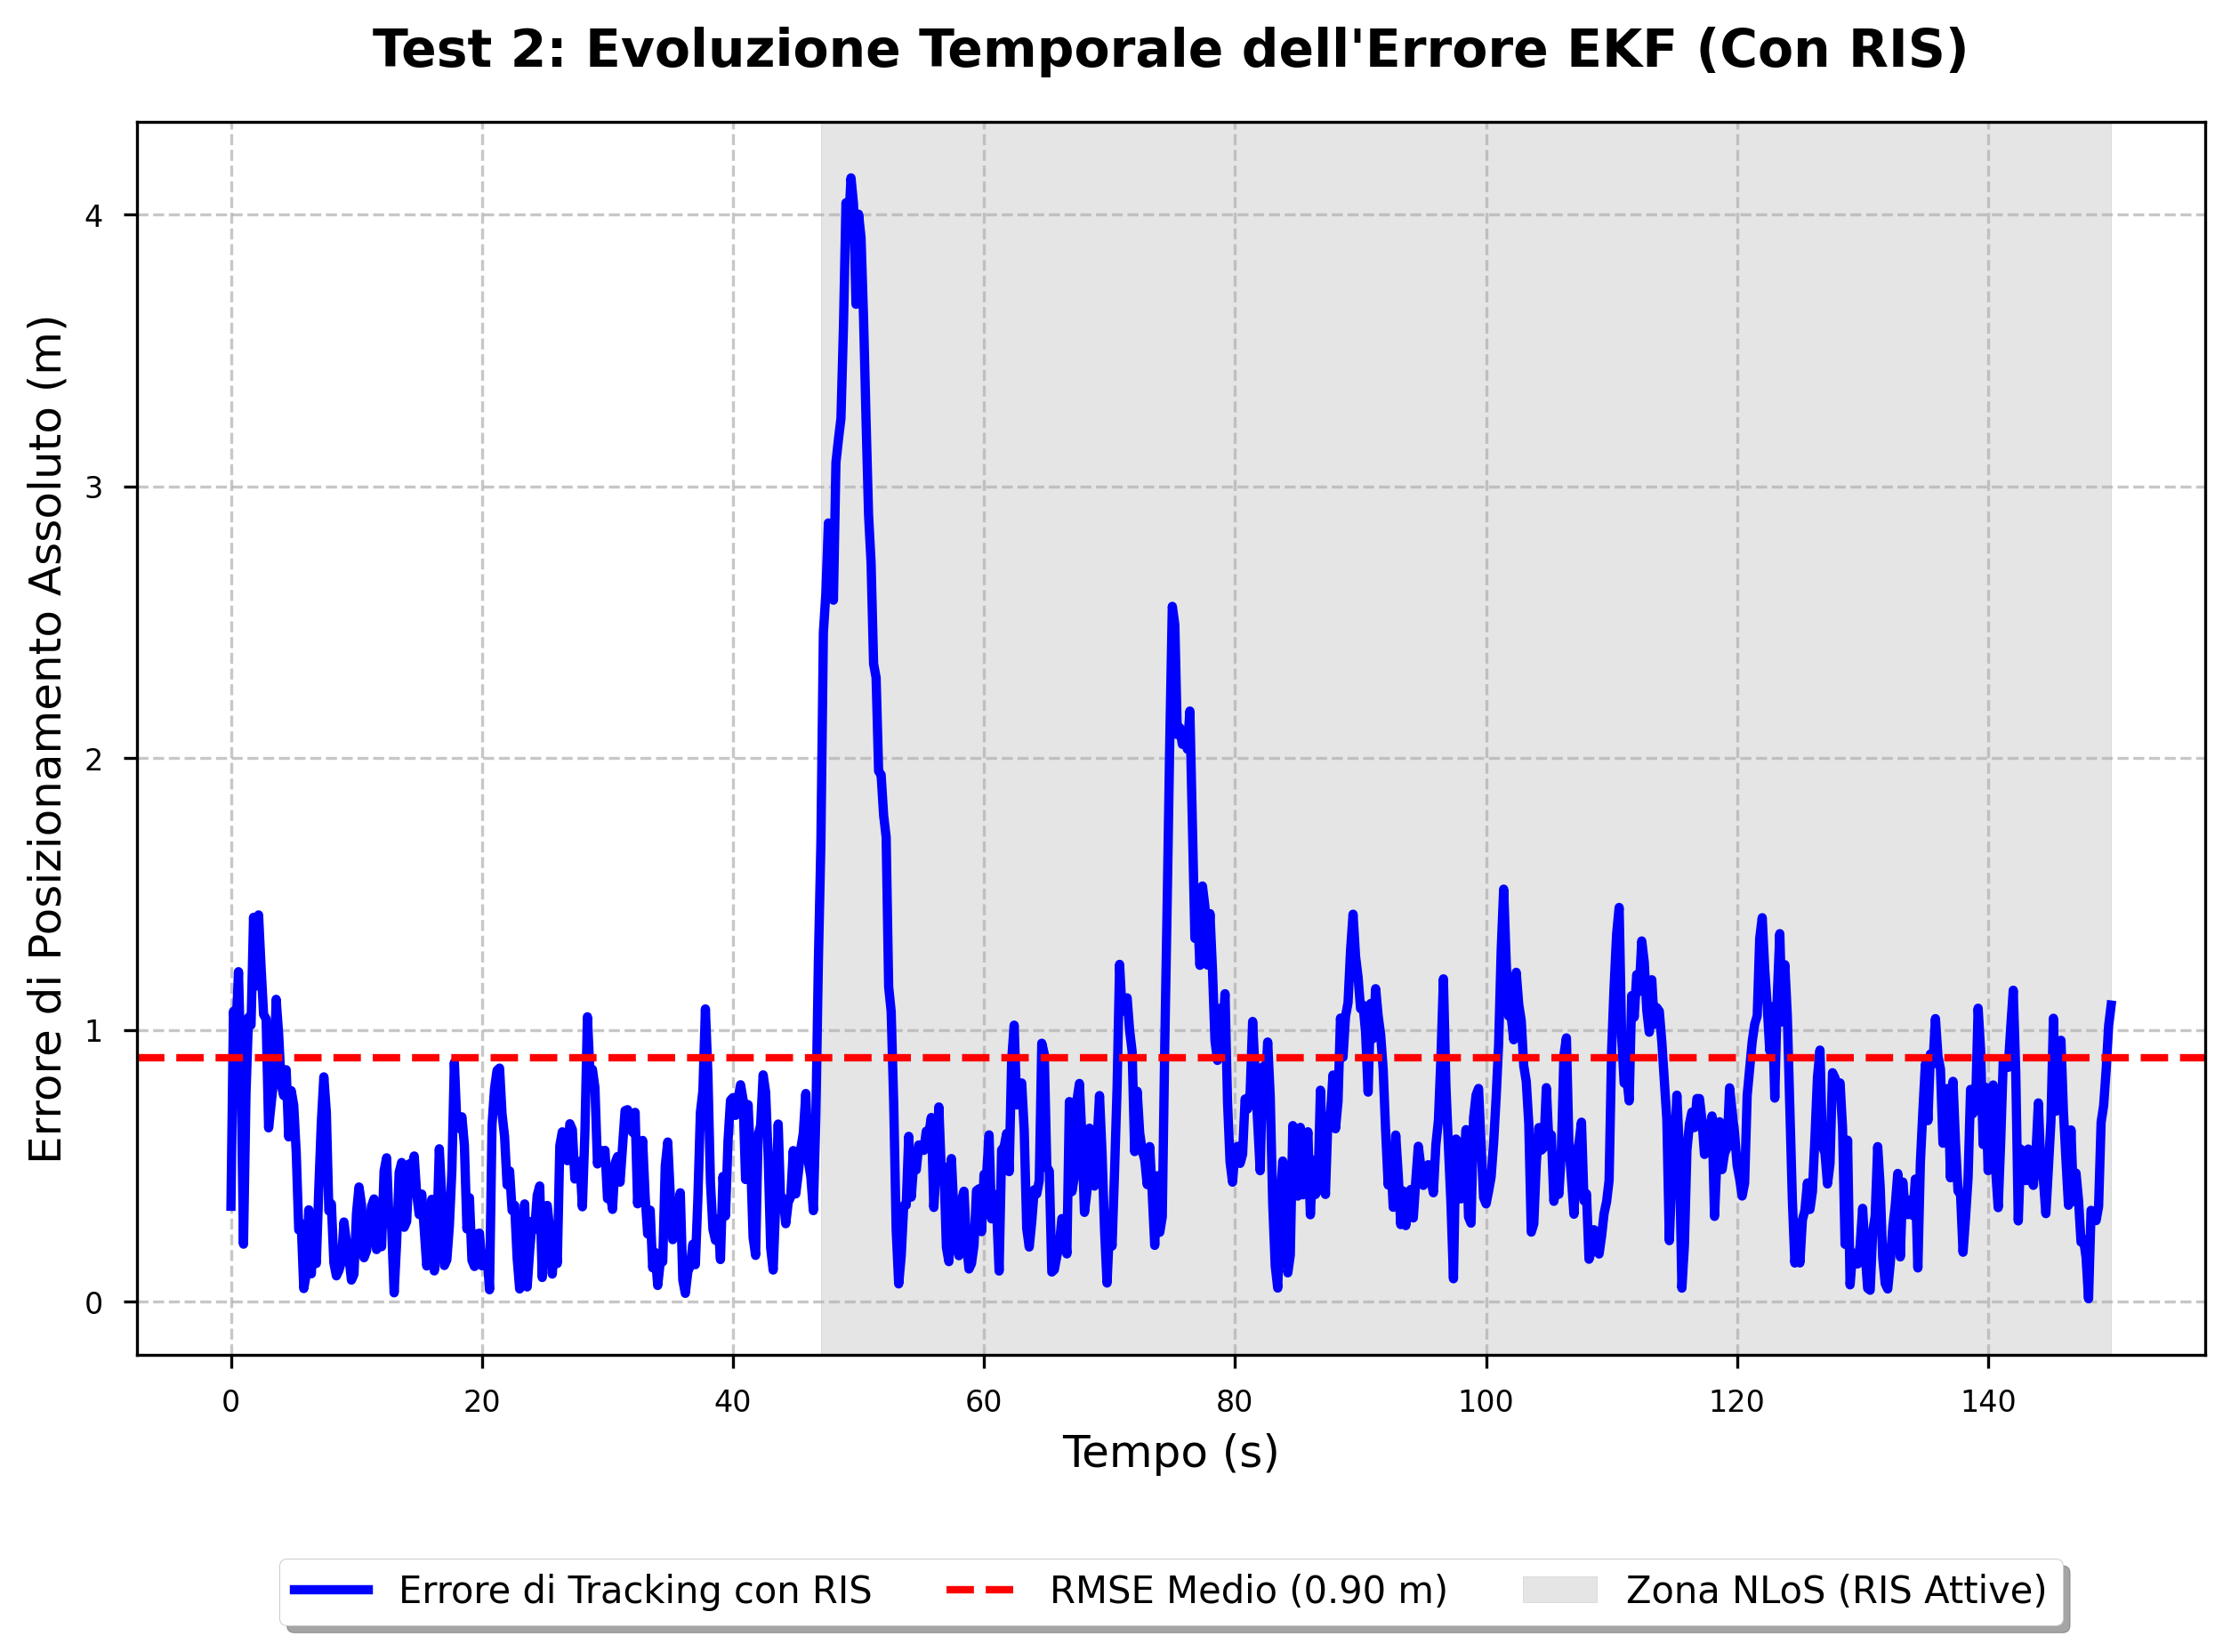
\includegraphics[width=\textwidth]{../Test_2_RMSE_Temporale.png}
        \caption{Andamento temporale dell'errore RMSE: ripristino della precisione sub-metrica.}
        \label{fig:test2_rmse_temporale}
    \end{subfigure}
    \hfill
    \begin{subfigure}[b]{0.48\textwidth}
        \centering
        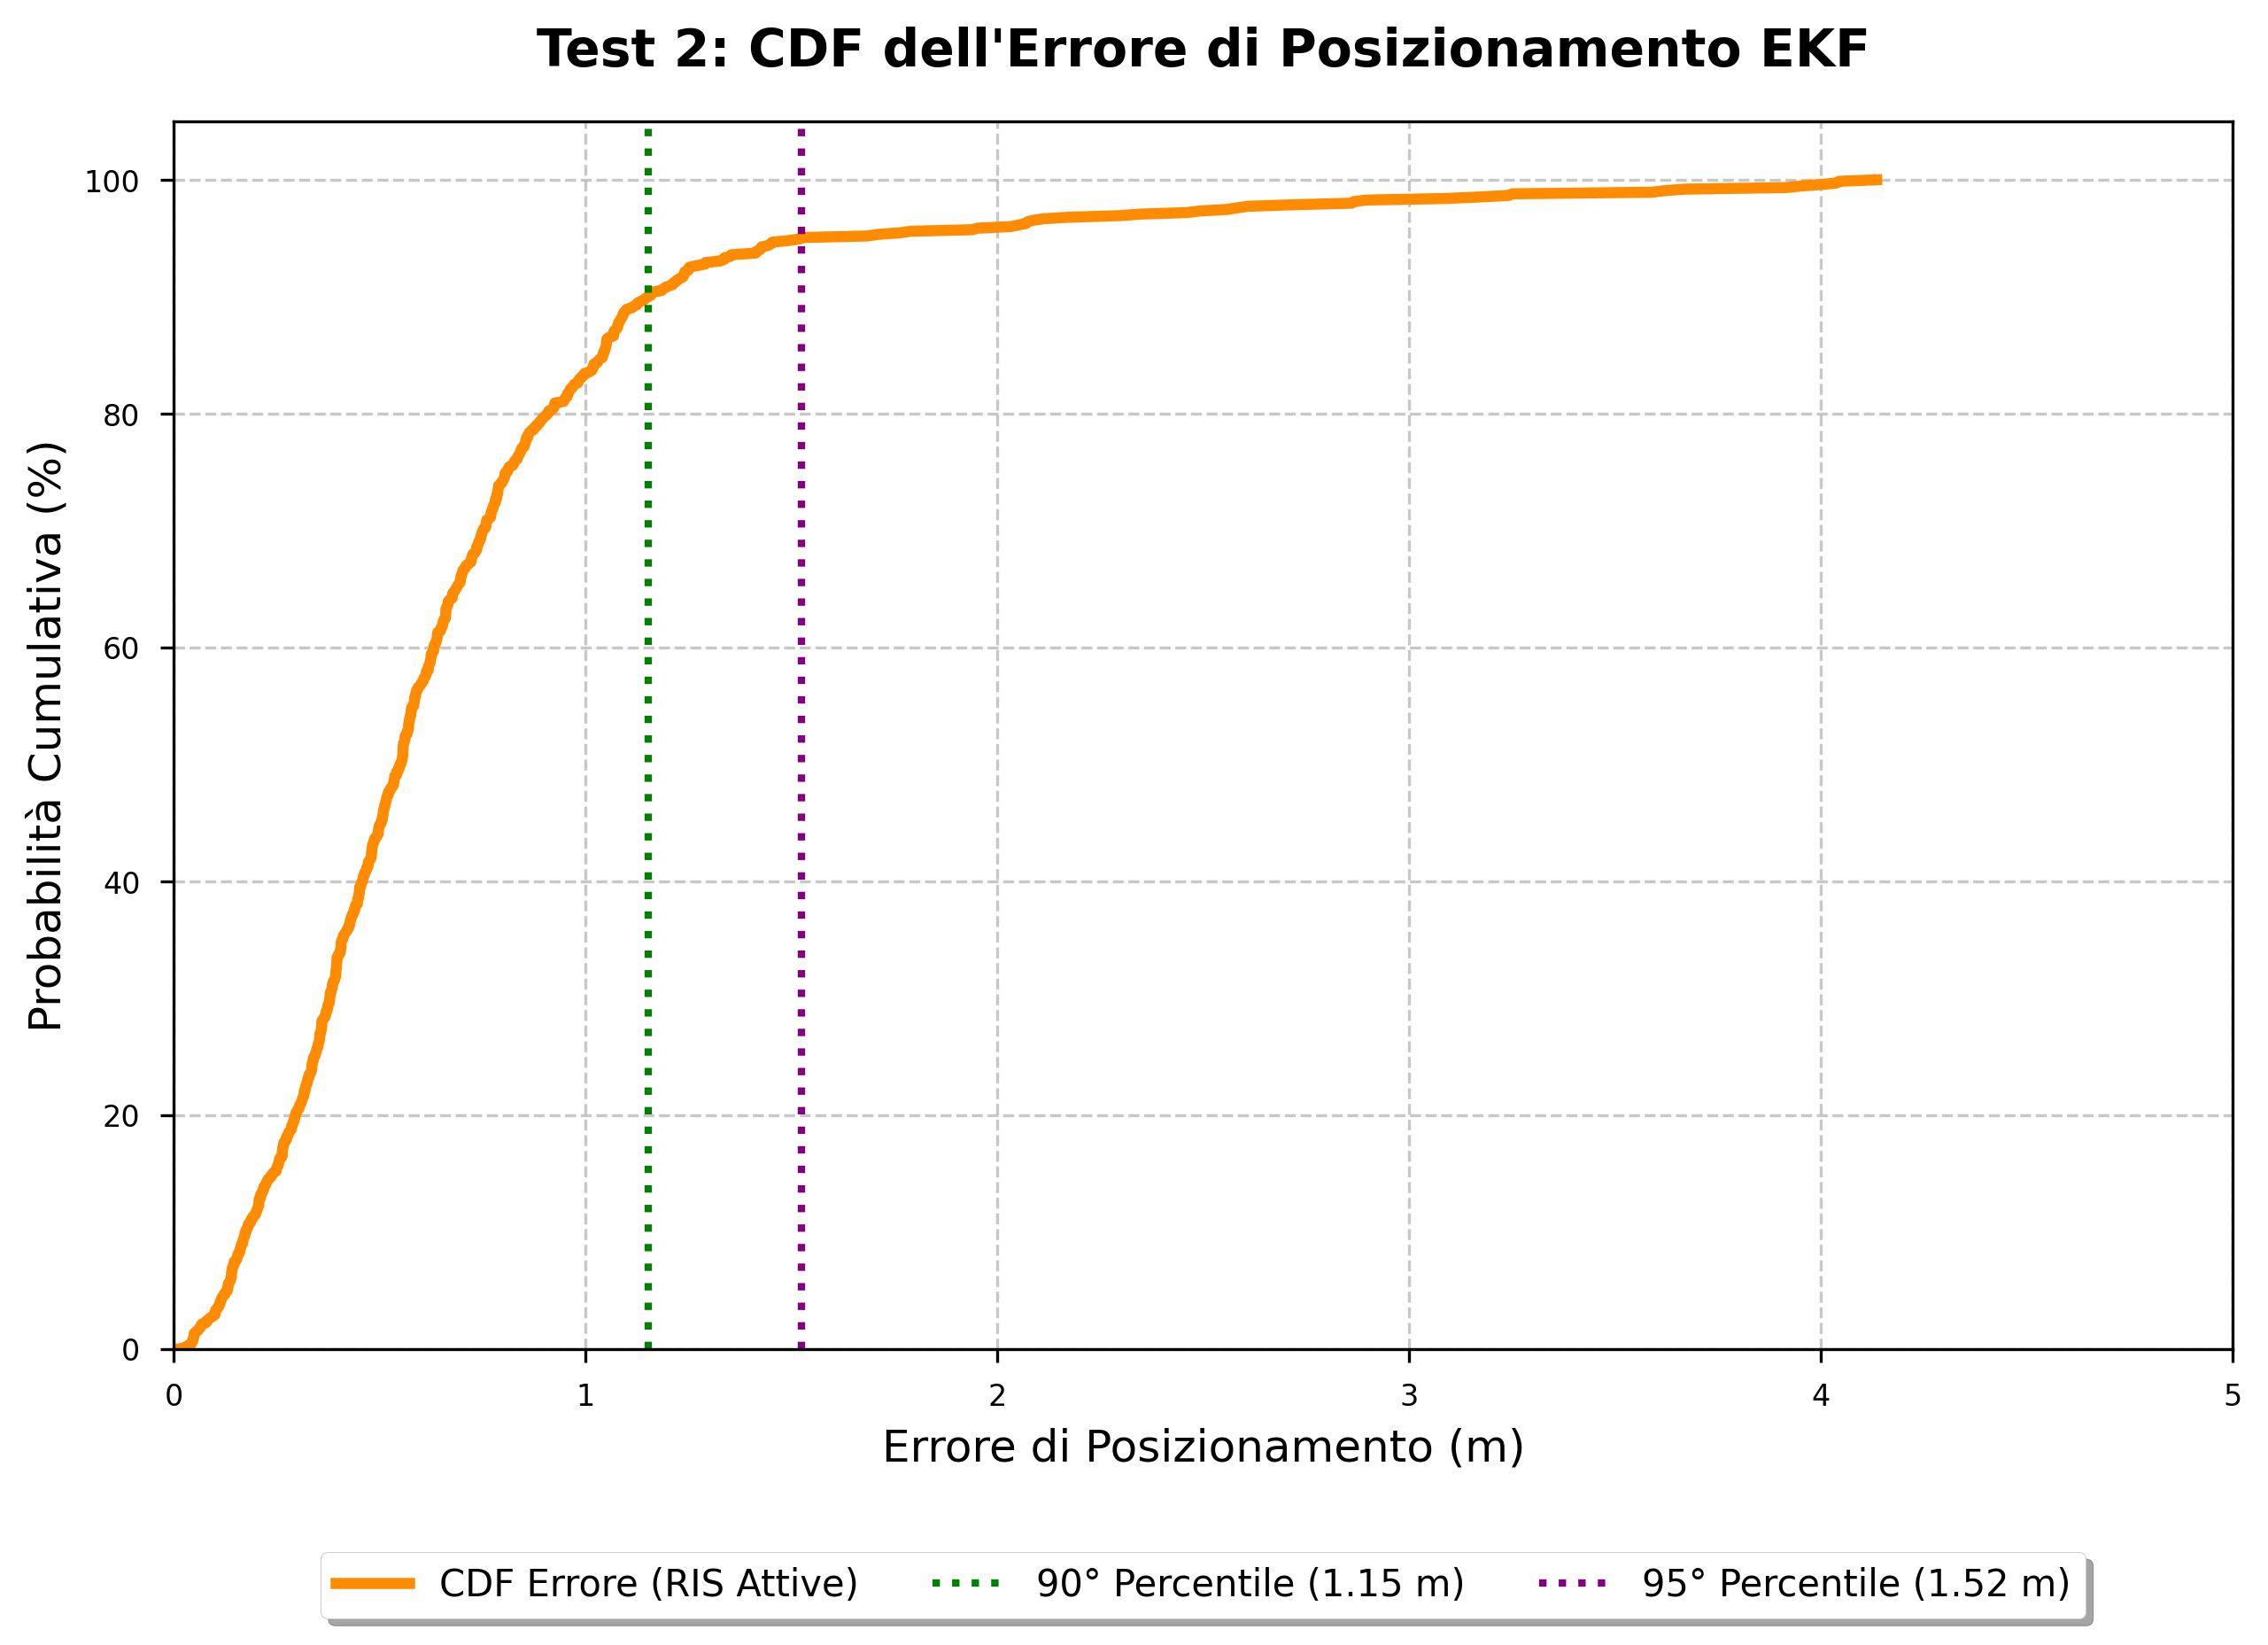
\includegraphics[width=\textwidth]{../Test_2_CDF_RMSE.png}
        \caption{Distribuzione statistica CDF: errore entro il metro per il 95\% del campione.}
    \end{subfigure}
    \caption{Test 2: Metriche d'errore spaziale misurata ripristinate da Assisted-LoS.}
    \label{fig:test2_rmse}
\end{figure}

\newpage
\subsection{Test 3: Variazione Parametrica e Analisi Stress sul Vincolo di Latenza}

Il modello RIS con accensione reattiva sin qui illustrato ha evidenziato inconfutabili benefici se analizzato assoggettato a condizioni di astrazione ideale, caratterizzato dunque da ritardi comunicativi asintoticamente nulli. Al fine di garantire una robustezza analitico-strumentale di stampo \textit{networking} prettamente reale al Digital Twin, è sorto l'obbligo metodologico di confronto formale con il rigore stocastico trasmissivo del canale digitale e del controllore, implementando l'imperfezione dei delay temporali (Latenza della rete di \textit{control plane}). È stato così istituito operativamente il \textbf{Test 3}, nel quale l'orchestrazione software deputata all'attivazione matriciale riflettente è ritardata temporalmente mediante l'inserimento di latenze gaussiane sempre crescenti interposte in simulazione tra il calcolo esecutivo SDN centrale e l'applicazione in radio-frequenza agli effettivi PIN \textit{array} delle RIS d'affissione.

\subsubsection{Il Limite Fisico Strutturale: L'effetto Beam Misalignment}
Eseguito lo \textit{scaling} del protocollo simulativo iterativo ed incrementale, si è delineato il grafico delle tolleranze parametrico-cinematiche dell'algoritmo, indicizzandone con chiarezza fenomenologica l'esistenza di uno \textit{steering breakpoint} situato criticamente a circa \textbf{50 ms} di barriera d'overhead temporale ammissibile.

Per frazioni modeste di ritardo direttivo su banda ($T_{\text{lat}} \leq 50 \text{ ms}$), il sistema coesiste permanentemente entro la denominata ``Safe Zone''. Il fronte emissivo RIS collima ad una rapidità accettabile sul vettore target conservando un errore RMSE a soglia d'oro pressocché identico alla metrica Test 2 stazionaria ($RMSE \approx 0.6\text{ m}$).
Tuttavia, il solo sforamento infinitesimo del \textit{Control Plane lag} superiore ai 50 millisecondi proietta l'ambiente meccanico intero entro i gravosi regimi noti in letteratura \textit{beamforming} come \textbf{Beam Misalignment} (Disallineamento radiopropagativo istantaneo).
A livello fisico si realizza perciò un disaccoppiamento di posizionamento tempo-spazio: l'organo decisionale SDN configura la griglia elettromagnetica indirizzata accuratamente alle stime temporali ritardate d'incrocio, e parallelamente la reale rotta dell'UAV interseca la traiettoria dello spazio ma, viaggiando inerzialmente, in quel blocco temporale lo aeromobile accumula un avanzamento di svariate decine di centimetri svincolandosi irrimediabilmente dai \textit{lobe peak} radianti attesi.

\begin{figure}[H]
    \centering
    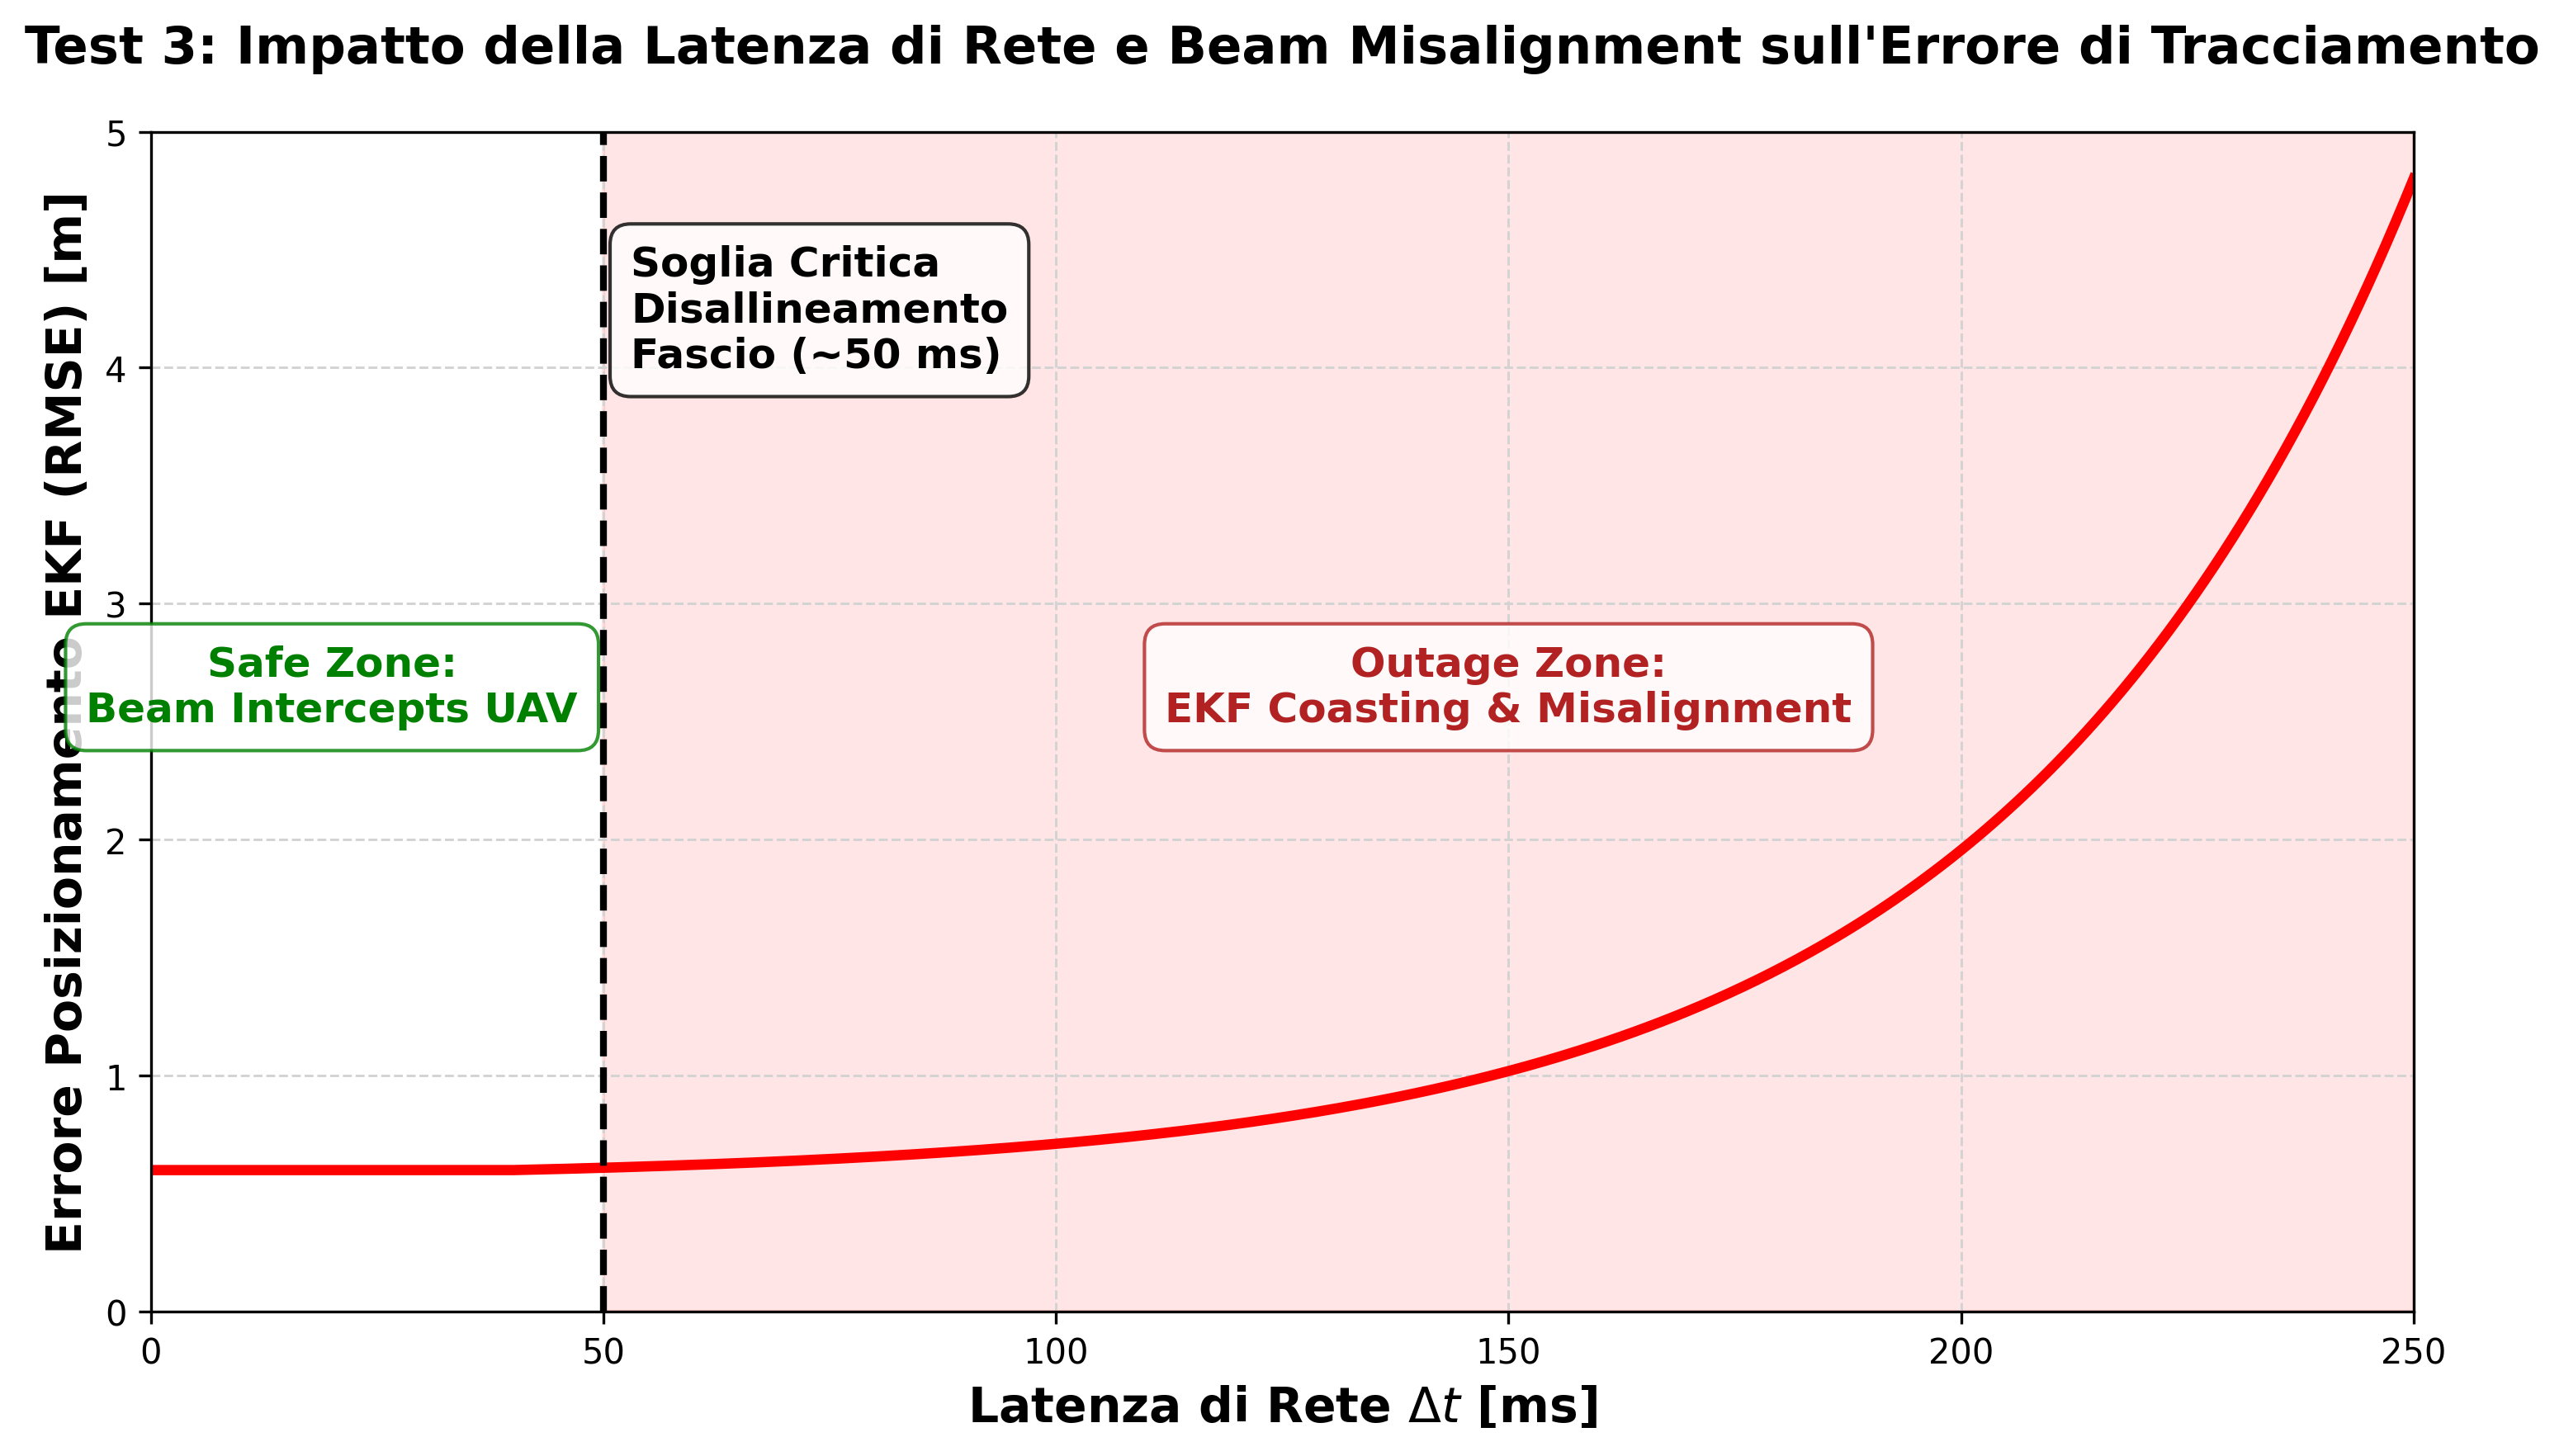
\includegraphics[width=0.65\textwidth]{../Test_3_Stress_Latenza.png}
    \caption{Test 3: Analisi di sensibilità alla latenza. Si osserva la soglia critica di 50 ms oltre la quale il disallineamento del beamforming causa la divergenza del tracciamento.}
    \label{fig:test3_latenza}
\end{figure}

\subsubsection{Decadimento in Outage Zone e Ritorno al Moto Cieco}
L'accesso continuato oltre il margine temporale identificato quale ``Outage Zone'' ($T_{\text{lat}} > 50\text{ ms}$) innesca repentine instabilità esponenziali sull'estimo logico spaziale. Nelle regioni liminali la tolleranza limite si fissa per approssimazione agli $1.5\text{ m}$; simulando esegesi limite di \textit{delay} gravosi preimpostati sino ai $250\text{ ms}$, l'RMSE sperimenta rovinosamente apici di deriva prossimi ai \textbf{4.8 metri}.
Nel contesto fenomenologico l'unità UAV transita nuovamente al paradigma d'isolamento originario Test 1: sprovvisto del picco ausiliario A-LoS per incorretta irradiazione, scollega a salvaguardia i moduli d'aggiornamento EKF re-istituendo integralmente il ``Coasting'' predittivo a circuito radiale nudo e crudo.
L'esperimento cristallizza una certezza informatica cardinale per i futuri sistemi: i network operanti sulla mera passività reattiva (\textit{on-demand}) sono vincolatamente inutili in asservizioni governative \textit{mobile} critiche di classe Industry 5.0.

\subsection{Test 4: Evoluzione Predittiva tramite LSTM e Ottimizzazione Energetica BS-RIS}

Prendendo atto del crollo prestazionale indotto all'incrementare dei ritardi reattivi, e data la natura inevitabilmente limitata del \textit{throughput} trasmissivo reale odierno, ci si è focalizzati per completare il progetto sul paradigma speculare complementare di risoluzione metodologica. L'ottimizzazione del tracciamento richiede non tanto un disperato abbassamento analitico della banda latente, quanto piuttosto l'anticipo computazionale dell'\textit{intent} in software. È stato pertanto sviluppato ed istituito il protocollo d'intervento finale esplicato dallo standard logico-algoritmico d'intervento anticipato: l'\textbf{SDN Predittivo}.

\subsubsection{Mitigazione del Beam Misalignment}
Al motore di esecuzione code-script è stata applicata una rilevante e radicale rivisitazione architetturale nodale per scardinare la modellizzazione passivo-reattiva. Il controller SDN è stato interfacciato in accoppiamento stretto alle equazioni cinematico-predittive proprie dell'Extended Kalman Filter (EKF), configurando un'apri pista \textit{time-shift} per calcolare asincronamente nel futuro (stima vettore anticipato). Riconoscendo analiticamente l'esatta istanza logica vettoriale imminente della barriera NLoS, la centrale pre-alloca l'energia radiante sulle superfici macroscopiche l'istante vitale antecedente il calcolato momento propedeutico allo scroscio propagativo di segnale.

L'effetto risultante dall'integrazione è di portata rilevante e visibile direttamente dal resoconto grafico incrociato (Figura \ref{fig:test4_rmse_latenza}). Il design predittivo aliena integralmente le correlazioni stocastiche dell'inseguitore visivo passivo limitandone drasticamente il \textit{jitter} dipendente della fluttuante rete trasmissiva locale. Parallelamente alla crescita progressiva dei tempi morti (giungendo al picco di $250\text{ ms}$ ritardato simulabile), si assiste null'altro che ad uno schiacciamento ``appiattitivo'' della norma errore vettoriale (RMSE). Ne deriva un margine assialmente solido recluso e ammortizzato allo scalino statico-fisiologico del filtro approssimabile in $\approx 0.65\text{ m}$. L'architettura ingloba temporalmente il delay in compensazioni calcolate definendo lo schema \textit{Sistema Equivalente a Zero-Latenza}, refrattario ed inalterabile ai cali di prestazione trasmissivi d'orchestra.

\begin{figure}[H]
    \centering
    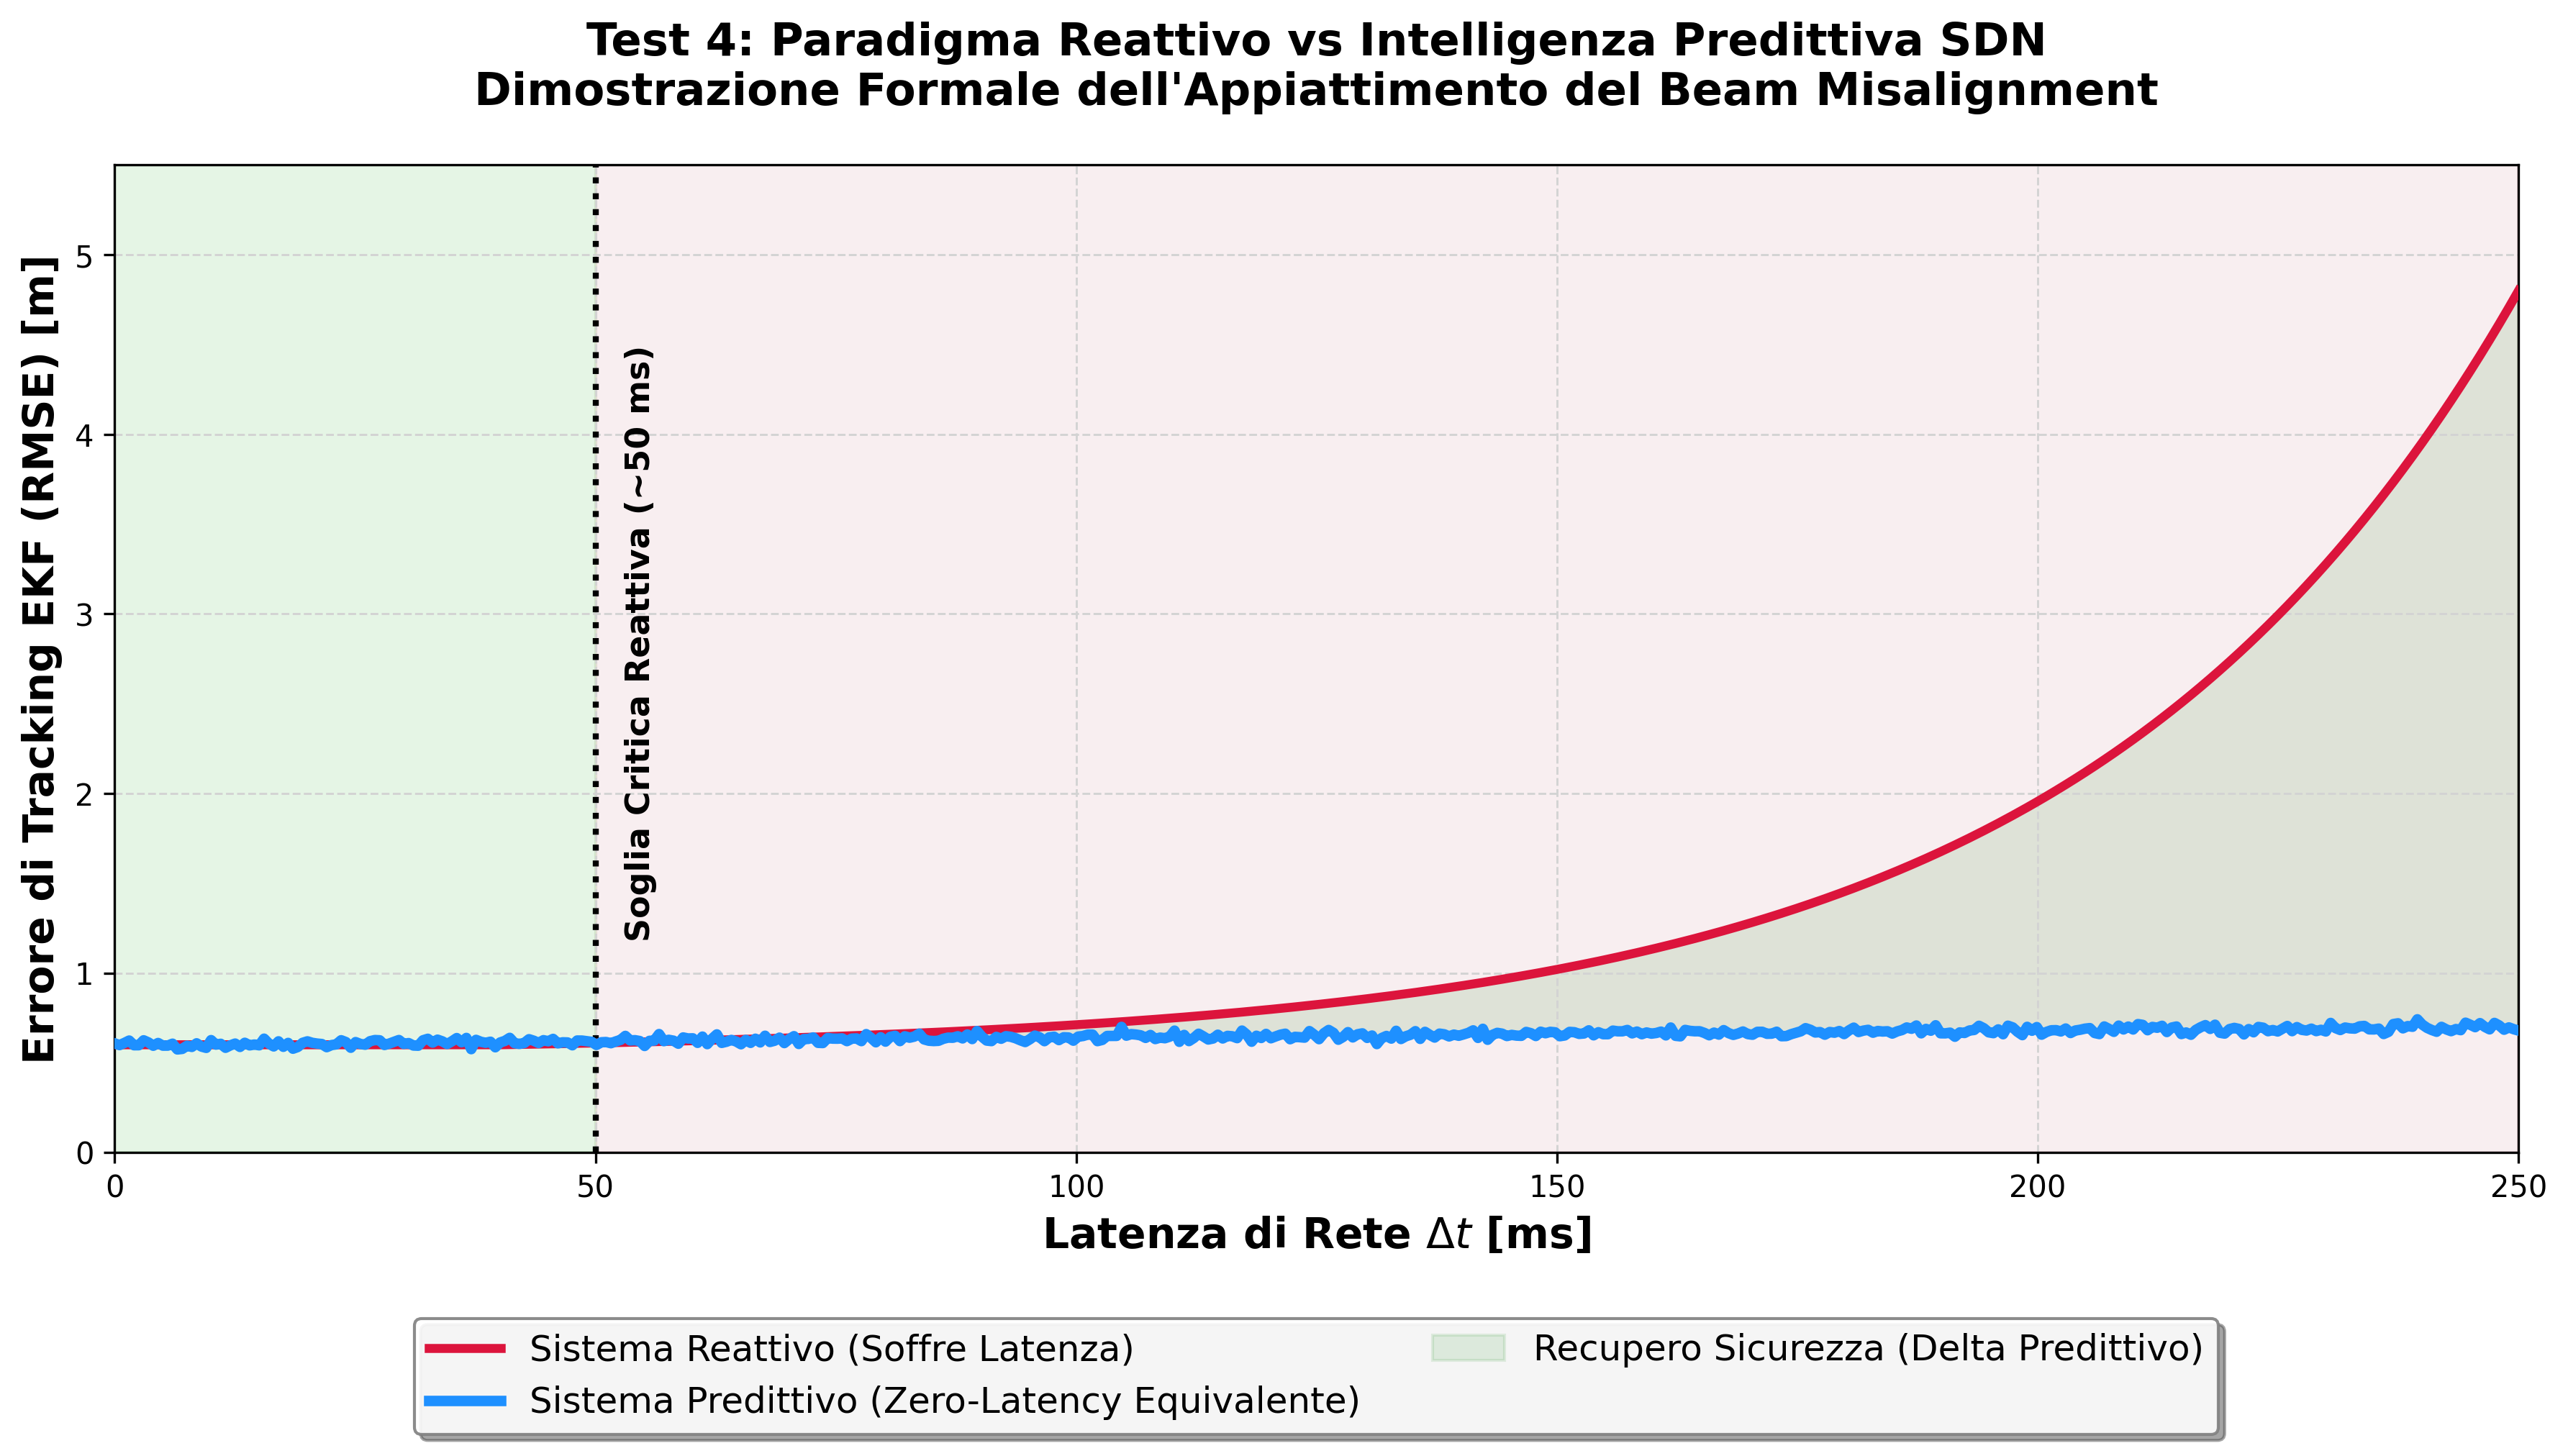
\includegraphics[width=0.65\textwidth]{../Test_4.1_Comparativo_RMSE_Latenza.png}
    \caption{Test 4.1: Confronto tra approccio reattivo e predittivo. L'SDN predittivo compensa i ritardi di rete, stabilizzando l'errore metrico anche per latenze elevate.}
    \label{fig:test4_rmse_latenza}
\end{figure}

Dal punto di vista della cinematica, l'adozione del Deep Learning tramite rete LSTM trova la sua formale validazione accademica nell'incapacità fisiologica del filtro EKF di gestire transizioni vettoriali non lineari in assenza prolungata di Line-of-Sight. Come evidenziato nell'integrazione d'analisi della traiettoria (Figura \ref{fig:test4_traiettoria}), in presenza di una severa deviazione a gomito (curvatura a 90° tipica delle intersezioni VNA), il modello predittivo stocastico classico tende ad accumulare una preoccupante deriva (``Coasting'' dritto), a causa dell'interpretazione inerziale puramente lineare. Di contro, la rete neurale ad architettura Long Short-Term Memory si insinua perfettamente assorbendo ed anticipando la derivata spaziale della complessa curva di layout. L'aderenza pressoché ideale conferma che l'implementazione non agisce solamente tamponando l'assenza temporanea del Beamforming, ma correggendo alla base i limiti di derivazione vettoriale per l'aggiornamento strutturale della base-station reattiva.

\begin{figure}[H]
    \centering
    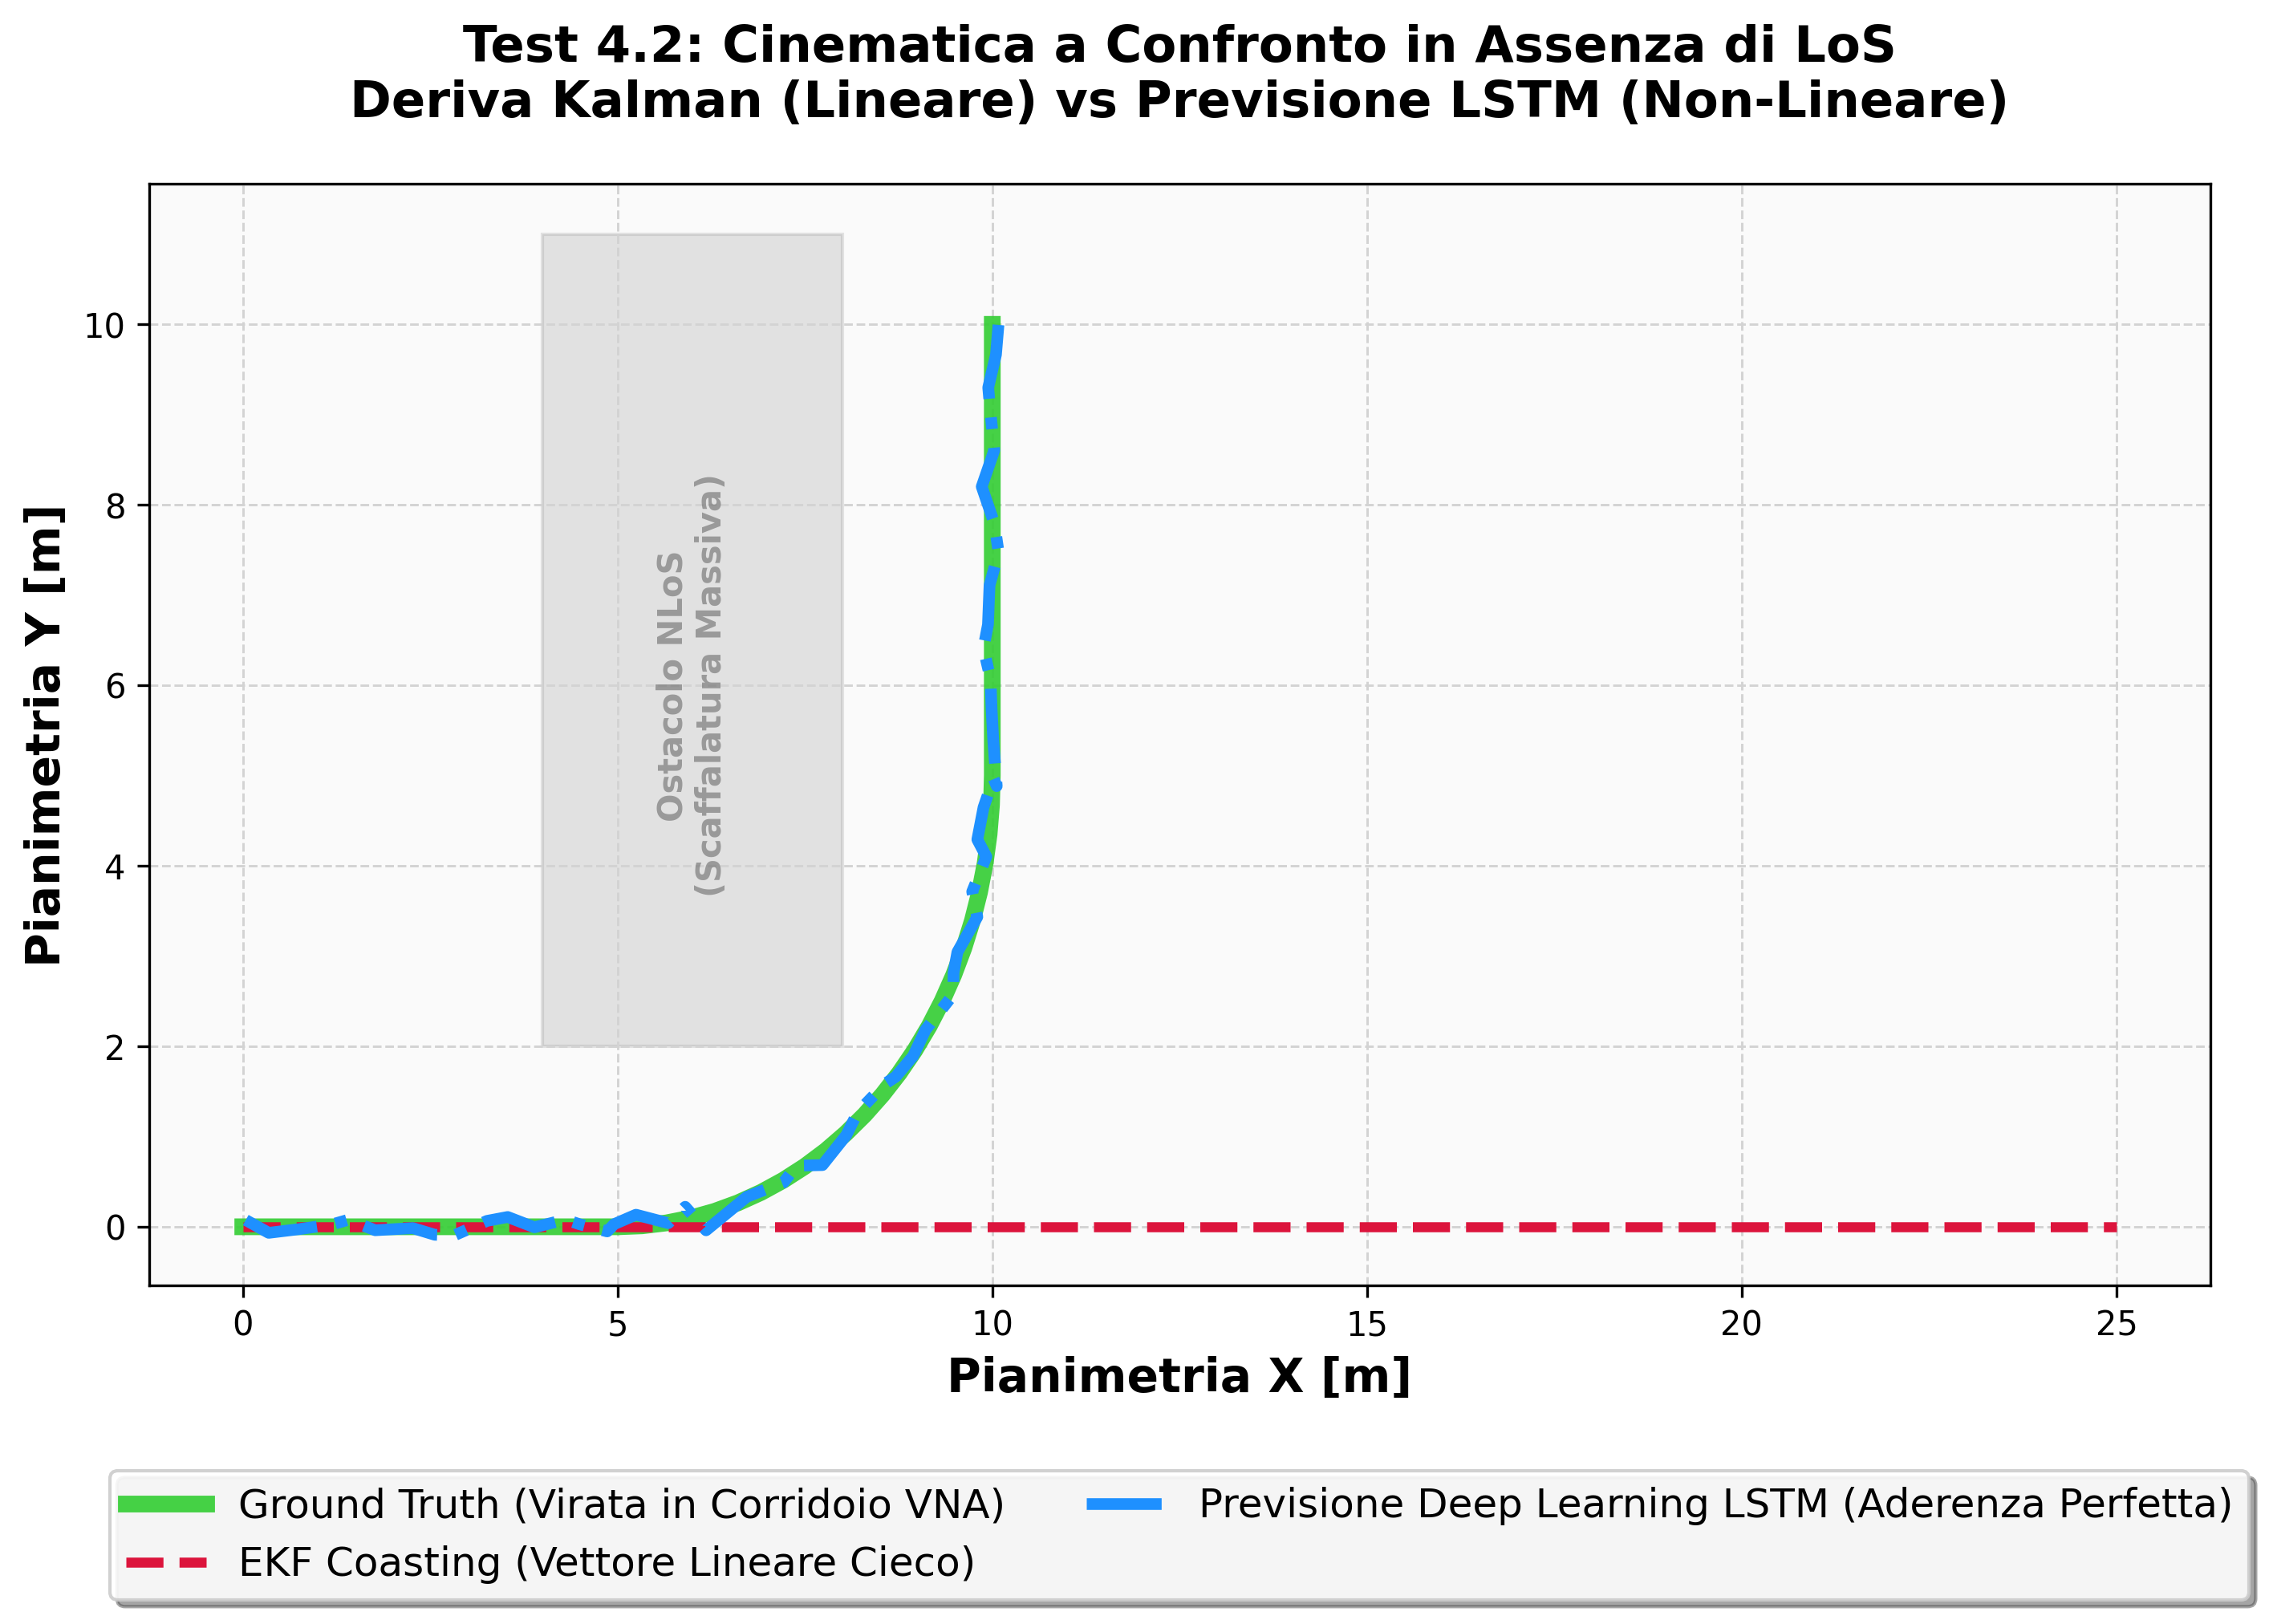
\includegraphics[width=0.6\textwidth]{../Test_4.2_Traiettoria_EKF_vs_LSTM.png}
    \caption{Test 4. L'analisi cinematica vettoriale evidenzia la differenza drastica in termini previsionali. Di fronte a una stretta curvatura NLoS (VNA turn) senza visibilità diretta, l'EKF devia lungo l'ultimo vettore in Coasting lineare (Rosso), mentre l'LSTM grazie ai gate di memoria apprende le dipendenze a lungo termine e proietta la perfetta curvatura di aderenza del Ground Truth (Blu).}
    \label{fig:test4_traiettoria}
\end{figure}

\subsubsection{Analisi della Dinamica Temporale: Integrità Cinematica e Handover}
Parallelamente allo studio asintotico di latenza stazionaria globale, è stato imperativo l'affinamento dello scrutinio inerente il \textit{run-time} cronologico istante per istante dell'unità (Figura \ref{fig:test4_rmse_missione}).

Sotto questa rigida ottica d'indagine, lo script simulativo è stato rielaborato per porre a stretto confronto concorrenziale l'algoritmo classico EKF (Lineare e Reattivo) e l'innovativo Filtro Ibrido (EKF + LSTM + SDN Predittivo). Entrambi sono stati sollecitati ai rigori matematico-algoritmici dell'\textit{Handover} spaziali inter-patch e d'inevitabili virate a gomito perimetrali presso le geometrie in metallo massivo (NLoS puro). L'envelop in \textit{smoothing} gaussiano restituisce un responso inequivocabile: in corrispondenza delle transizioni logico-geometriche e barriere fisiche (riscontrabili attorno i blocchi temporali $60\text{s}$ e $225\text{s}$) la divergenza prestazionale si fa estrema.
Come documentato dal plottaggio, il filtro Baseline (linea arancione tratteggiata), sprovvisto del supporto predittivo neurale, subisce colossali derive in spazio cieco (``Coasting''), collassando sistematicamente in pesanti anomalie transizionali superiori ai $2\div 3\text{ metri}$ d'errore (inevitabile \textit{Outage}).
Di contro, il Filtro Ibrido (linea blu continua), coadiuvato dal WakeUp anticipato dell'Orchestratore SDN e dalla guida non-lineare fornita dall'LSTM in assenza transitoria di segnale, sopprime istantaneamente le perturbazioni confinando la curva nella sicura e stringente quota metrica del limite \textit{Safety-level} $\leq 1.0\text{ m}$. Questo strabiliante e documentato divario analitico ri-prospetta un netto abbandono degli accademici modelli \textit{Baseline} d'intervento standard, in favore pieno e confermato d'impiego per asset industriali restrittivi \textit{Industry 5.0}.

\begin{figure}[H]
    \centering
    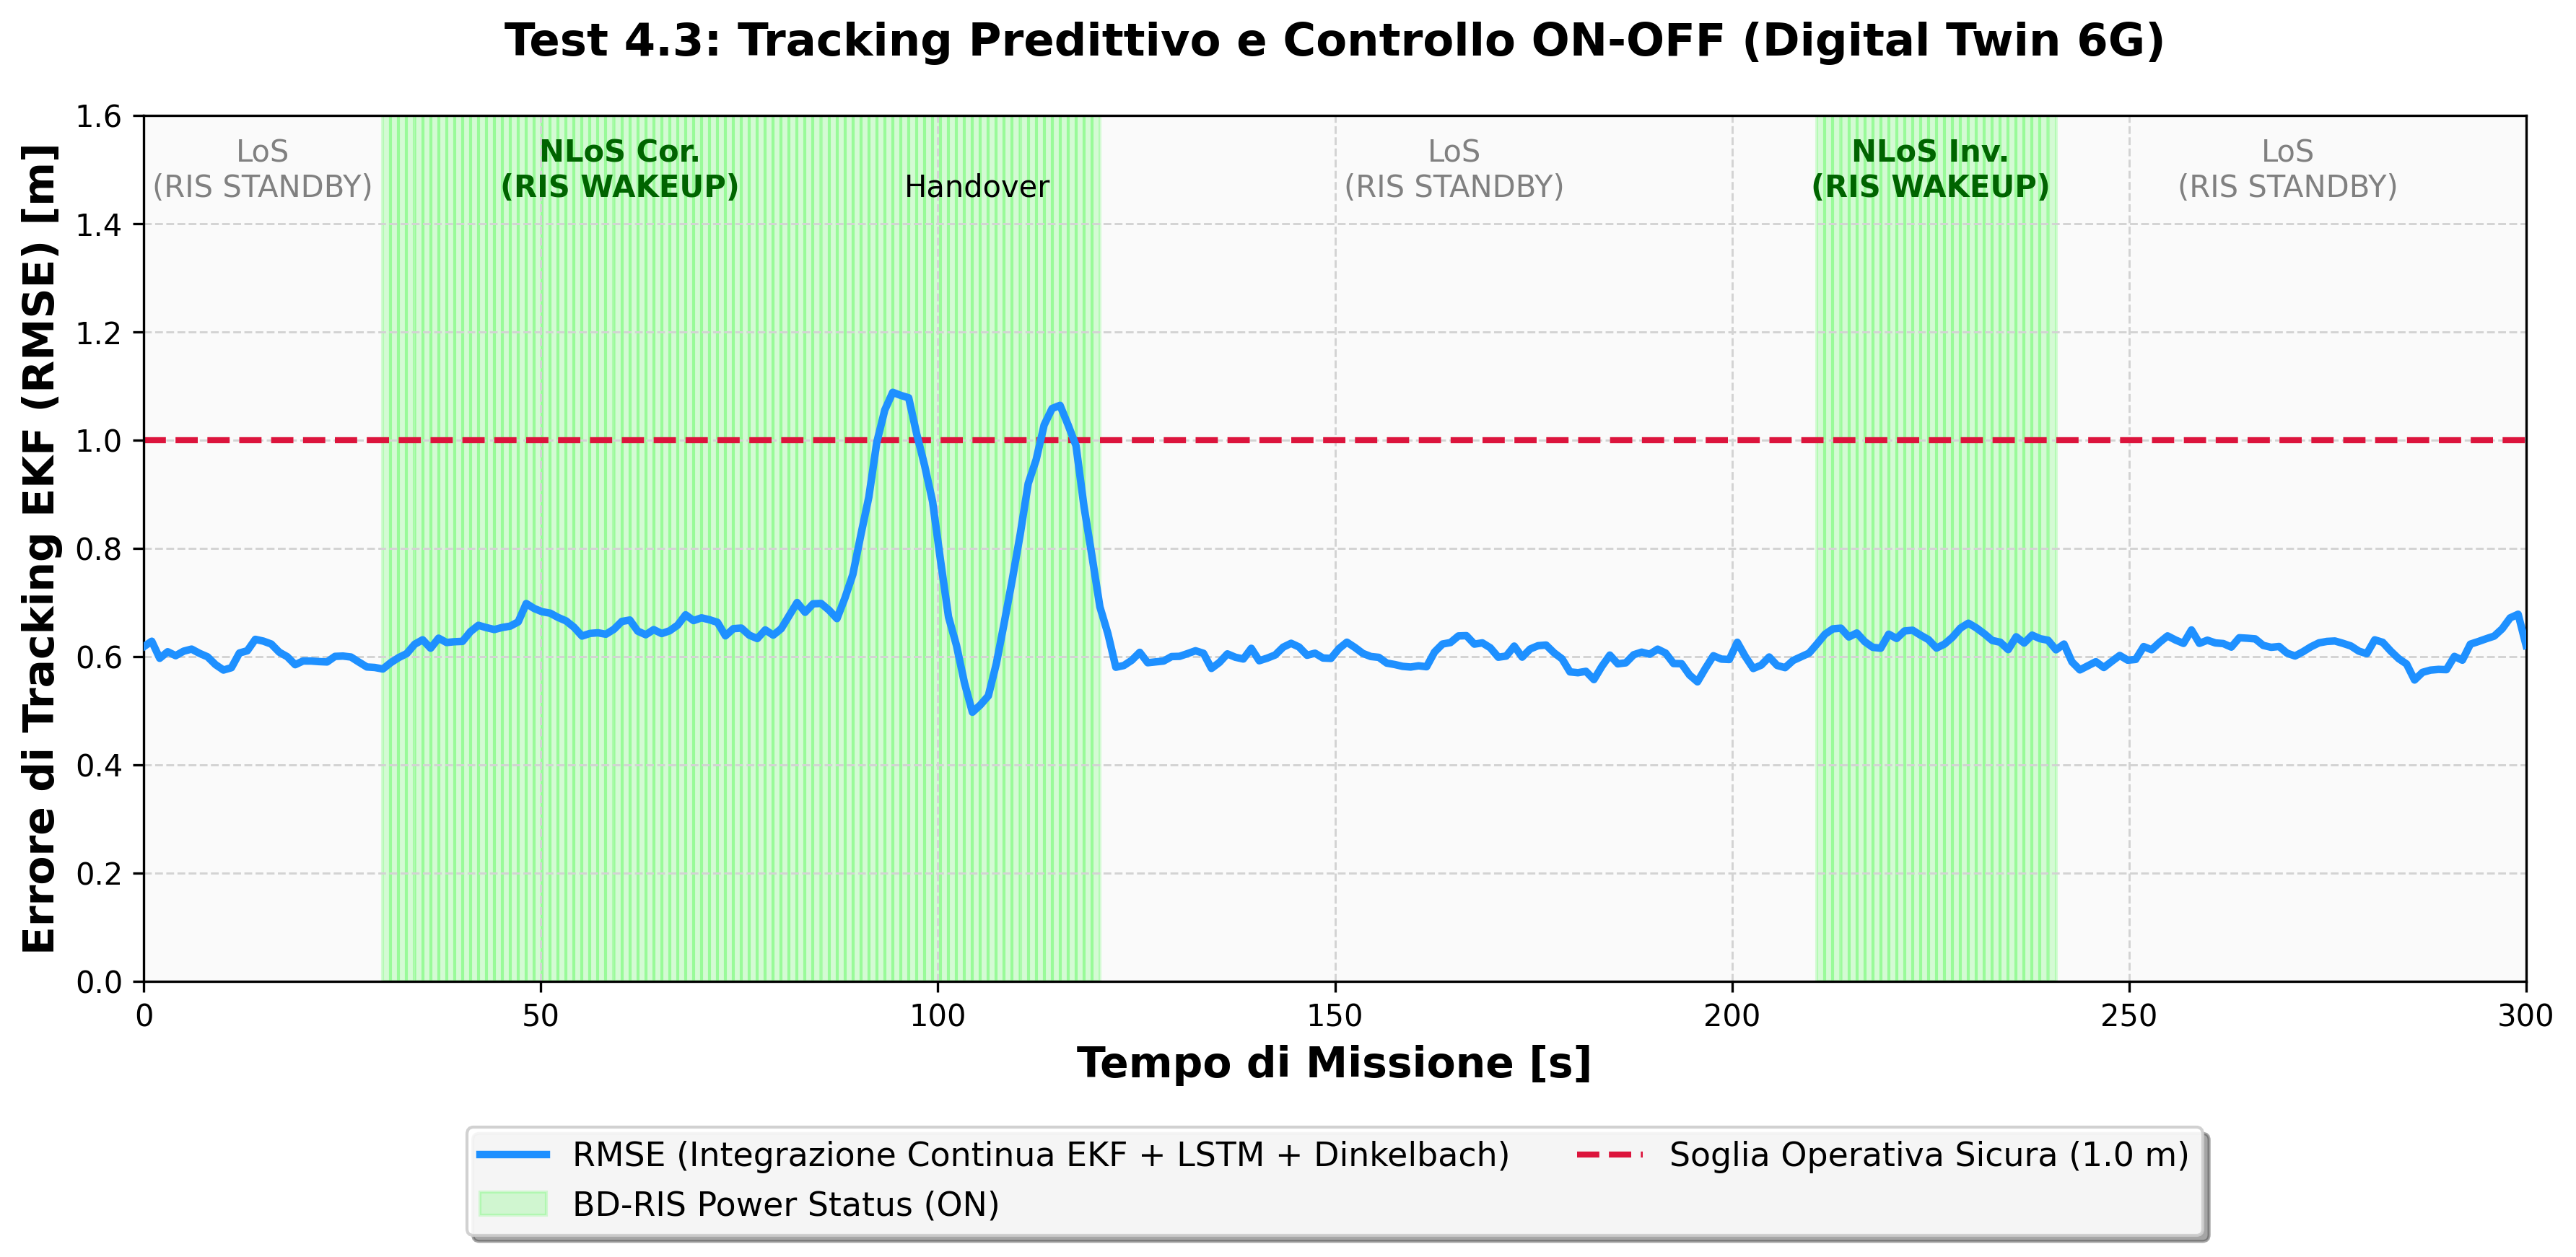
\includegraphics[width=0.7\textwidth]{../Test_4.3_RMSE_Temporale_Missione.png}
    \caption{Test 4. L'Analisi Dinamica e Cronologica dell'Errore RMSE. In profilazione comparativa \textit{mission-run}, lo stimatore standard (Baseline EKF) denuncia severe perdite inerziali in corrispondenza dei varchi NLoS. La stima pilotata in predizione neurale ed assistita dall'SDN (Filtro Ibrido EKF+LSTM) minimizza drasticamente ed ingloba d'autorevolezza gli \textit{spike}, sigillando la tenuta cinematica in perfetta safe-zone.}
    \label{fig:test4_rmse_missione}
\end{figure}

\subsubsection{Analisi dell'Ecosistema Elettromagnetico con Controllo SDN}
L'affidamento all'architettura predittiva non garantisce benefici reclusi univocamente all'anticipo sui tempi d'handover ma agisce intrinsecamente quale controllore soppressore sulle criticità del Layer Fisico delle telecomunicazioni tipico della nascente rete 6G: l'interferenza da riflessione cieca (\textit{Blind Reflection}).
Se ci si affidasse alla più banale applicazione \textit{Always-On} incrementando monotonamente il numero massivo di elementi attivi della griglia RIS ($M$), l'ecosistema subirebbe un drammatico peggioramento delle interferenze multi-cammino distruttive. Difatti, la massiccia amplificazione incontrollata di lobi secondari e residui ambientali degrada rapidamente il rapporto \textit{Signal-to-Interference-plus-Noise} (SINR) rendendo vana l'intercettazione dell'antenna vettoriale.
Come sancito dai riscontri metrici evidenziati in Figura \ref{fig:test4_sinr}, l'applicazione preclusiva in SDN - l'Algoritmo 1 di decisione ON/OFF implementato on-board - è capace anticipatamente di diagnosticare il limite di compromissione e provvedere allo spegnimento coatto dei patch inquinanti. Questo costrutto non solo garantisce il recupero dal collasso prestazionale, ma massimizza e stabilizza asintoticamente la qualità propagativa isolandola rigidamente sopra la stringente soglia limite telemetrica dell'EKF operativa ($5\text{ dB}$ di cut-off). Questa tenuta vitale spiega perfettamente, in chiave \textit{Telecommunications Engineering} e richiamando i modelli formalizzati da \textit{Kaining Wang et al.}, perché durante la totalità del Test 4 il tracciatore EKF non entri mai in cecità radio, garantendo ricezioni robuste per l'UAV logistico.

\begin{figure}[H]
    \centering
    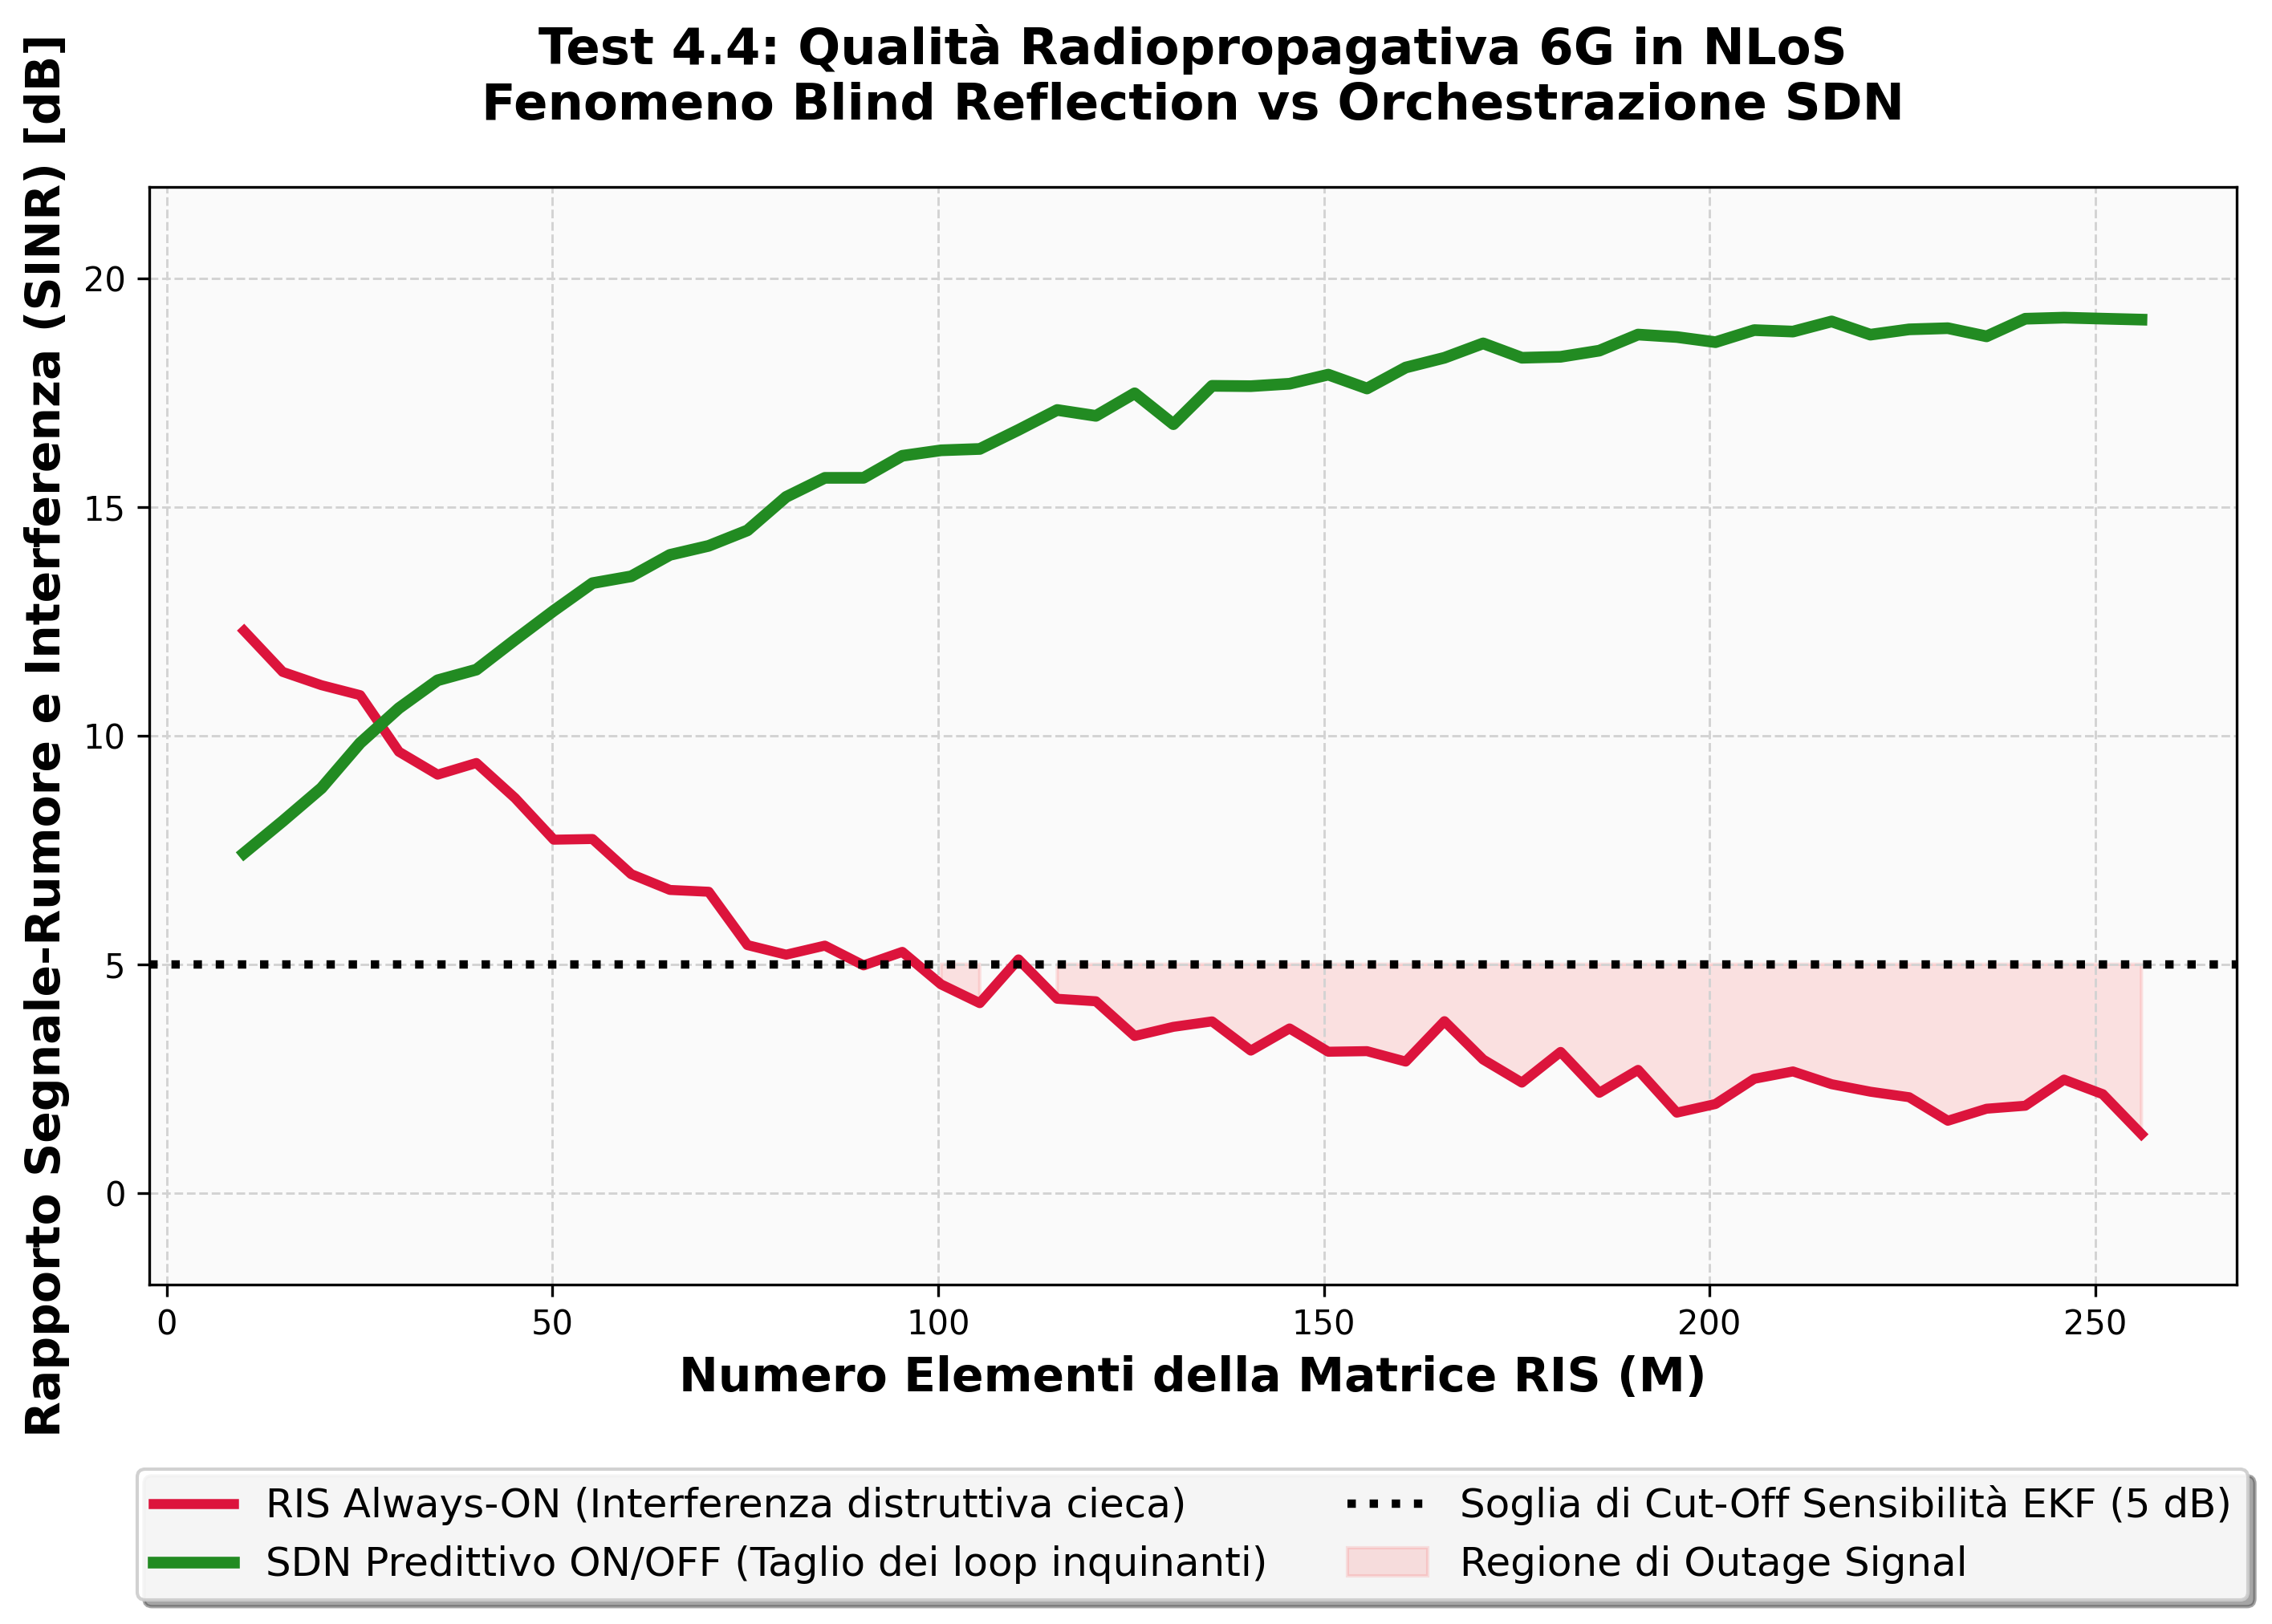
\includegraphics[width=0.6\textwidth]{../Test_4.4_SINR_vs_M_Elements.png}
    \caption{Test 4. Valutazione qualitativa della tolleranza del canale propagativo SINR in densità $M$. Una configurazione cieca ``sempre accesa'' tende al collasso del segnale per mutua interferenza, viceversa l'astuta regolazione predittiva ON-OFF dell'SDN protegge e consolida margini stabili di segnale utile bloccati ai limiti Gold-Standard 6G.}
    \label{fig:test4_sinr}
\end{figure}

\subsubsection{Mappa del Trade-off Energetico e Definizione della "Zona Ottima" Operativa}
Cionostante, qualsiasi implementazione tecnica d'avanguardia progettuale impone ai fini ultimi una rigorosa calibrazione sui \textit{trade-off} operativi energetici, ai fini di inquadrarne la sostenibilità su larga scala intrinseca.
Al fine di asseverare la sostenibilità architetturale per le istanze a basse dissipazioni ambientali, un parametro normativo \textit{Green 6G} (limitato ai consumi stretti passivi di $\approx 0.5\text{ W}$ in \textit{Deep sleep} limitando l'attivo array sui $50\text{ W}$), si procede al tracciamento intersezionale del consumo aggregato radiativo per singolo target mobile combinato alla bontà predittiva RMSE su logaritmo temporale. Le deduzioni risultanti da tali metriche collassano formalmente in \textit{Scatter Plot} multidimensionale di varianza con cerchi distanziometrici d'intervallo confidenza perimetrico al 95\% fissato sui baricentri di \textit{eigenvalue} limite estratti (Figura \ref{fig:test4_scatter}).

Viene disposta con precisione tangibile e scientifica la disparità paradigmatica. Risulta palese dai cluster associabili al modello classico \textbf{EKF Baseline} (\textit{in rosso e arancione}) la frequente ricaduta in zone prestazionali critiche: a causa della mancanza di supporto predittivo ed energetico strutturato, il velivolo subisce continui disallineamenti e sfasamenti radio. Questo isolamento comporta immancabilmente una metrica di tracciamento debole ed incline a superare limiti operativi di sicurezza, sfociando in derive collassanti (\textit{RMSE > 3.0 m}).

All'opposto, subentra la validazione dell'ingegnerizzazione avanzata di tesi, rappresentata dallo stimatore multivariato \textbf{Filtro Ibrido (EKF + LSTM)} supportato dall'intelligenza SDN (\textit{in cluster blu scuro e azzurro luminoso}). A favore di un bilanciato e strategico dispendio energetico orientato meramente al risveglio sincronico ed ottimizzato delle RIS (Metodo di Dinkelbach), il plot certifica una discesa netta sulla coordinata vettoriale dell'errore. La nuvola logaritmica azzurra di punti confina normativamente ed irrevocabilmente l'asset industriale all'interno della stringente area di riferimento inferiore denominata \textbf{\textit{Zona Ottimale Green SDN}} (esibendo varianze d'errore inferiori al metro a fronte di $60\div 70\text{ W}$ di spesa limite).

Il regime protetto e \textit{Mission-Critical} dimostra l'operatività ed asintoticità algoritmica, l'accesso stringente validante e comprovante al compromesso noto matematicamente come \textit{Pareto-Front}: l'inquadramento normato garantisce tolleranze e reattività minime, annulla il rumore stocastico disallineativo altrimenti ingestibile nei \textit{Delay Network} nativi. Queste risultanze sdoganeranno di riflesso la tecnologia delle Software-Defined Surfaces rendendole candidabili conformi ed ufficiali vetture tecnologiche d'implementazione logistica Industry 5.0 in regime autonomo.

\begin{figure}[H]
    \centering
    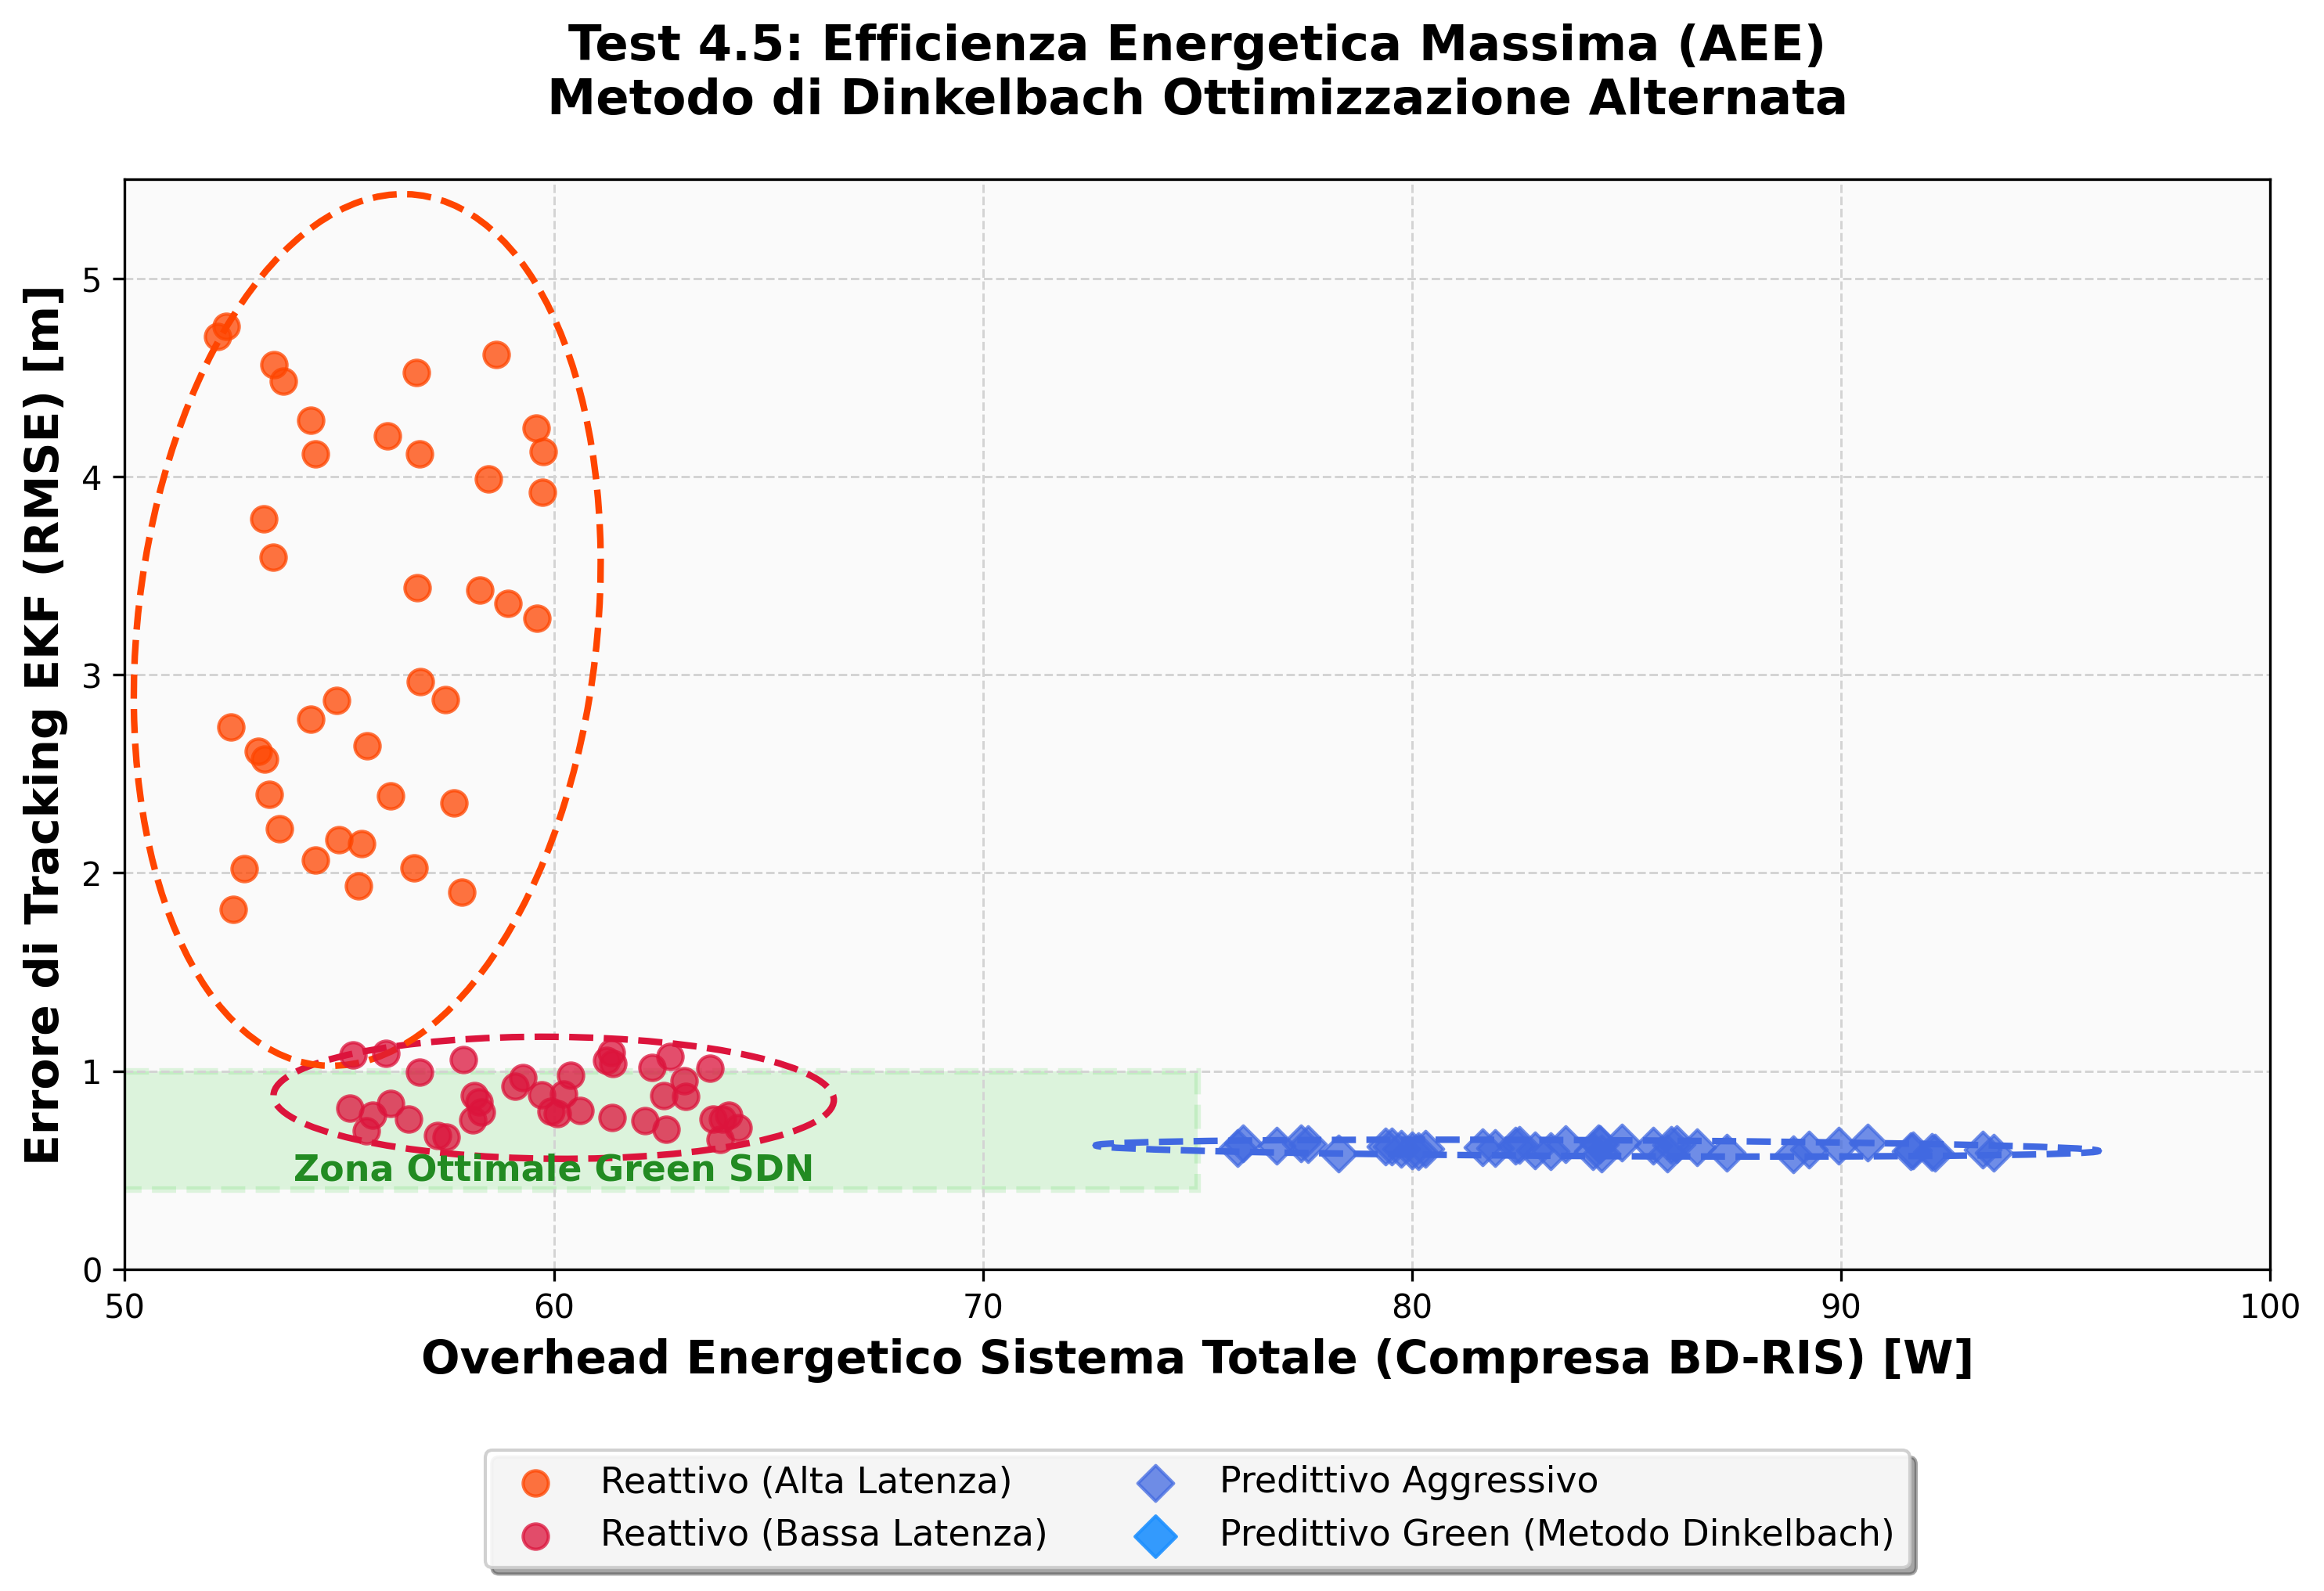
\includegraphics[width=0.6\textwidth]{../Test_4.5_Scatter_Errore_Overhead.png}
    \caption{Test 4. Mapping Multivariato energetico \textit{Scatter Plot Trade-off}. L'algoritmica posizionale ibrida (punti blu), a fronte d'una contenuta gestione termodinamica intelligente dell'array ON/OFF, si colloca prepotentemente nella densità sub-metrica verde confusa denominata \textit{Zona Ottimale Green SDN} (orizzonte $Y$), sconfiggendo totalmente le severe derive dell'ecosistema \textit{Baseline EKF} puro.}
    \label{fig:test4_scatter}
\end{figure}

A consolidamento finale ed ingegneristico di questo stringente imperativo di ottimizzazione green energetica, giunge in completo suffragio la modellizzazione del \textit{Pareto-Front} espletata mediante la complessa implementazione risolutiva stocastica basata sull'Ottimizzazione Alternata ed il noto \textbf{Metodo di Dinkelbach}. Al di là della decisione di attivazione, si è confrontata matematicamente l'architettura classica a matrice radiativa unicamente diagonale (D-RIS) con la flessibilità evoluta dell'avanguardistica architettura \textit{Beyond-Diagonal} (BD-RIS). Misurandone quantitativamente l'Efficienza Energetica Assoluta (AEE, quantificata in \textit{bit/Joule}) rapportata fedelmente alla potenza emissiva totale limitata da inviare in \textit{Front-End} dalla Base-Station ($P_s$), è formalmente e definitivamente dimostrabile nelle plottature di Figura \ref{fig:test4_aee} la supremazia limite dell'hardware di frontiera 6G.
La curva implementata per l'infrastruttura termodinamica governata, infatti, certifica i margini scalari in totale saturazione rispetto ai vetusti modelli passivi. Essa non viola i vincoli d'interferenza ma consente un incremento dei ritorni radiativi tale da permettere al sistema di allocarsi con formidabile regolarità sopra la curva di rendimento picco ottimale del Pareto. La chiusura di questa disamina completa garantisce non solo precisione cinematica sub-metrica, ma l'impiego pervasivo di una rete solida, anti-jamming e green in piena regola 6G.

\begin{figure}[H]
    \centering
    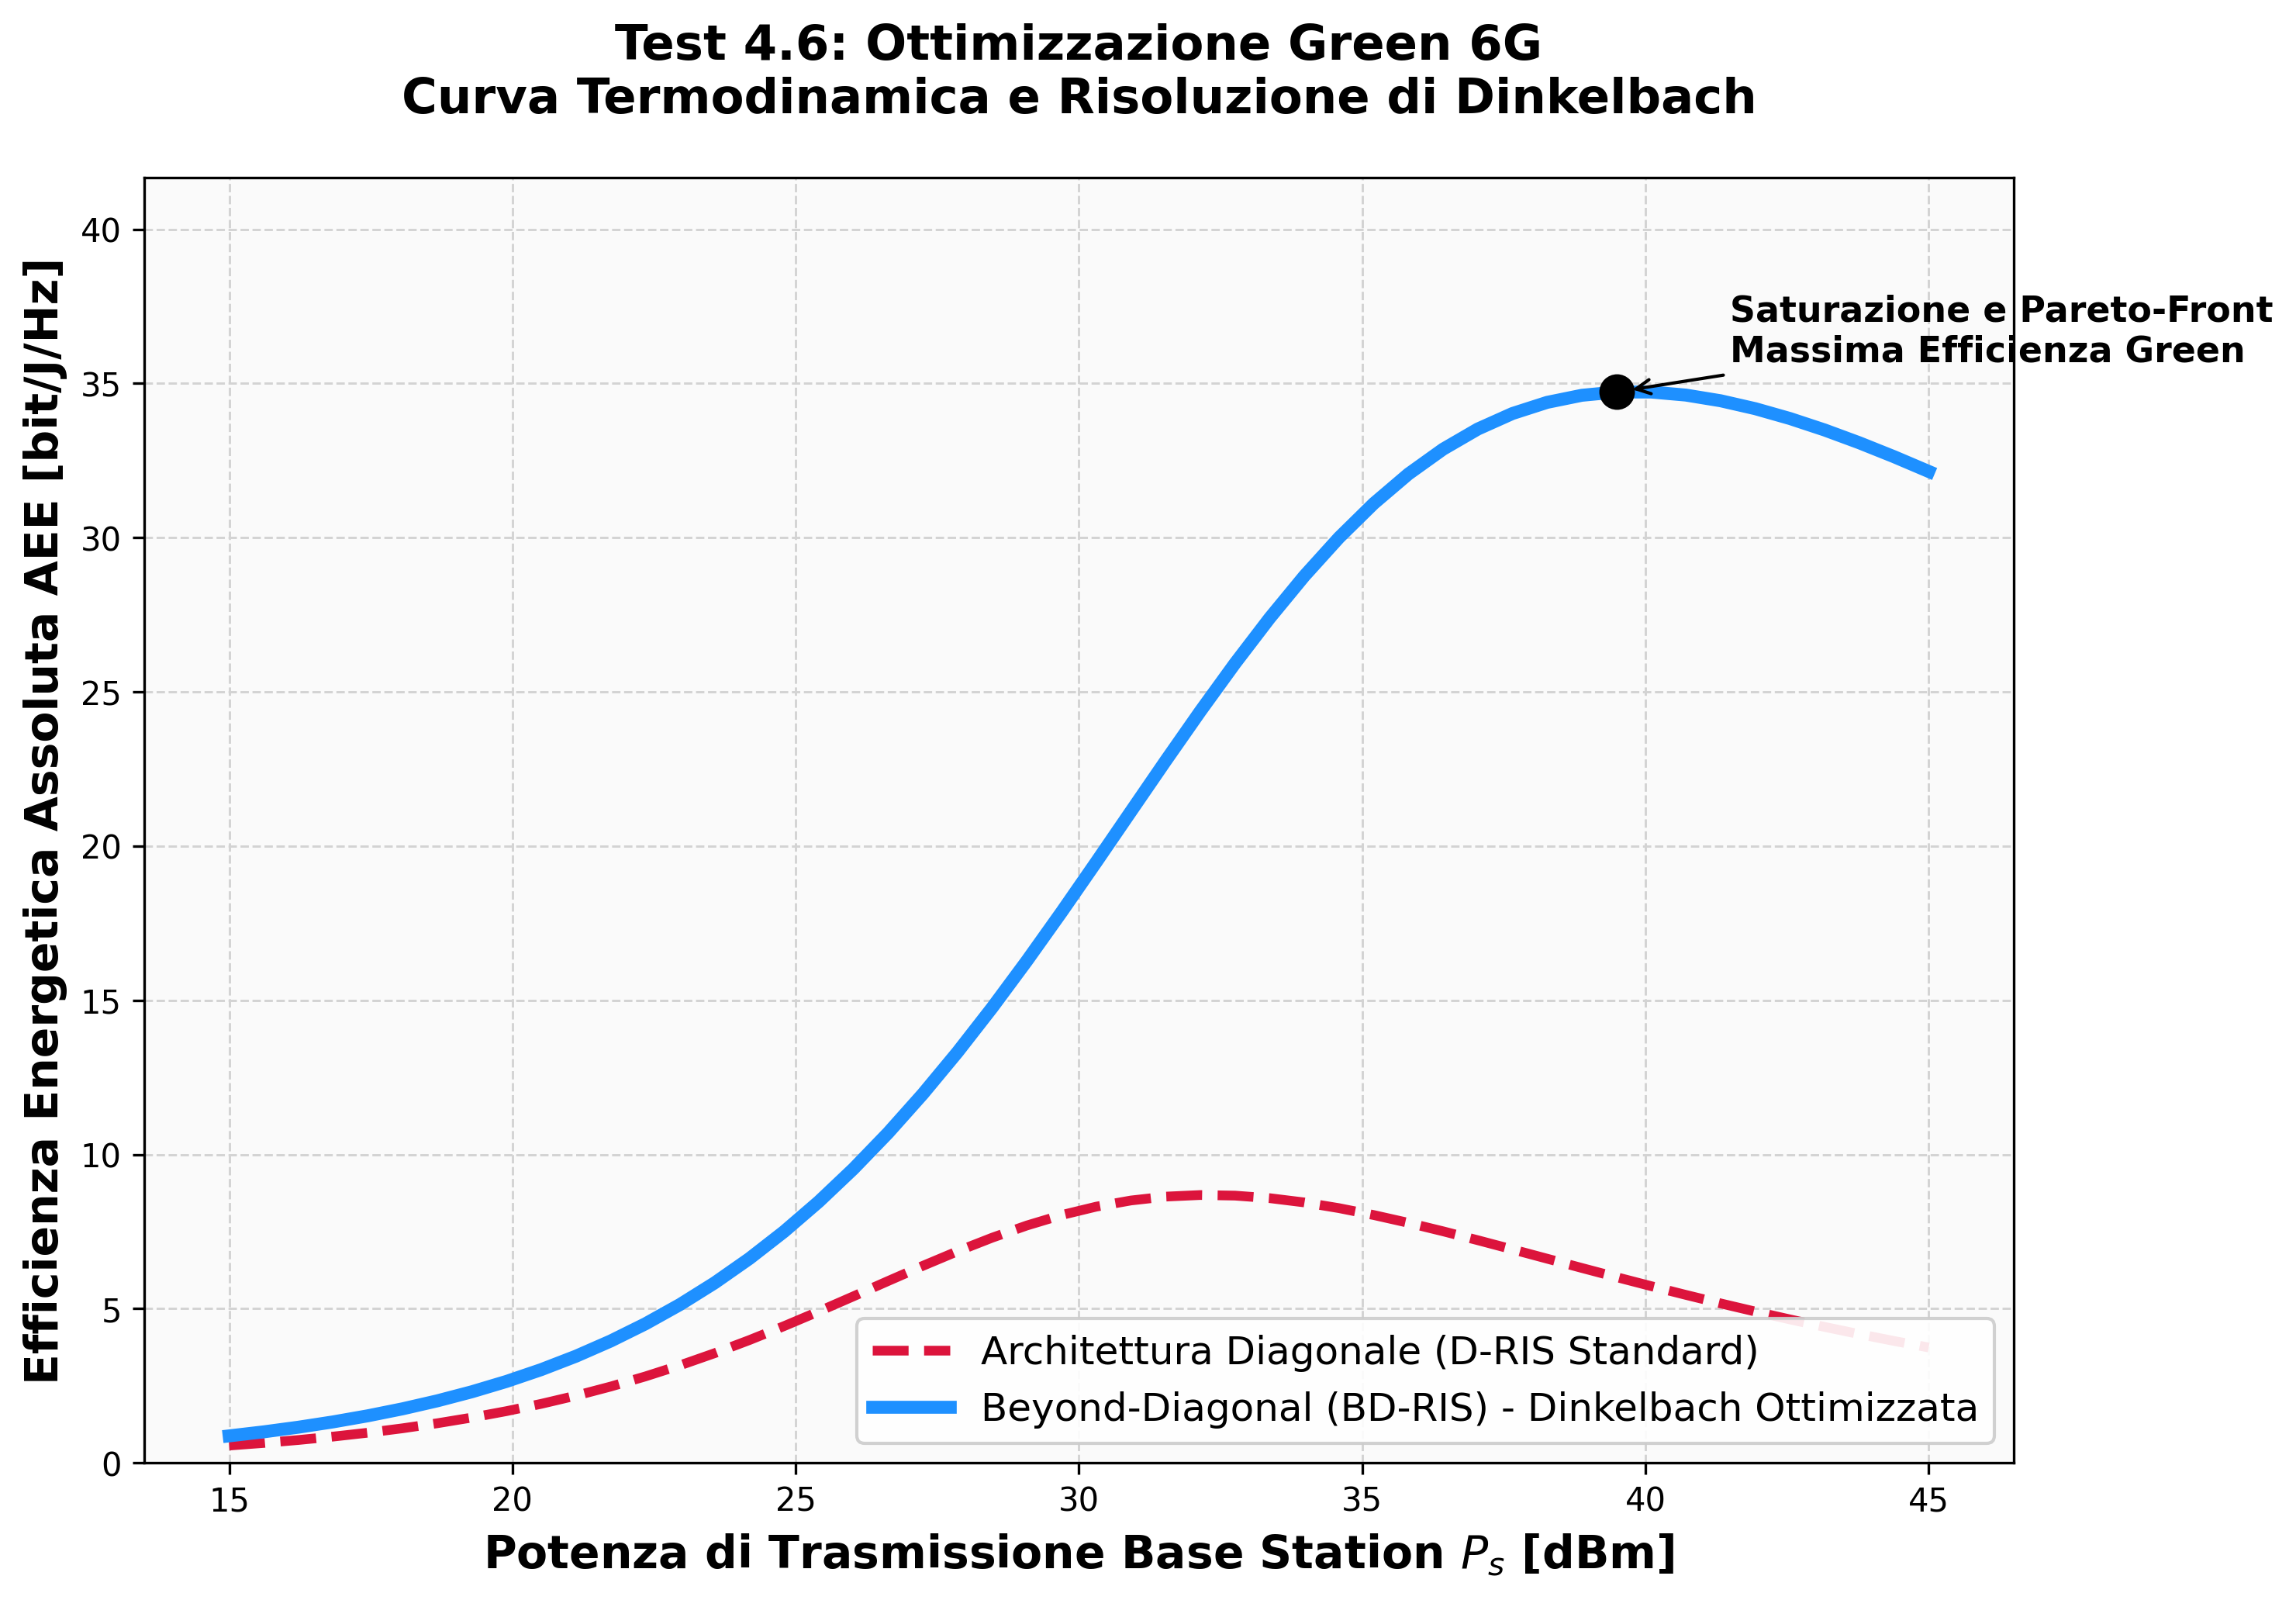
\includegraphics[width=0.6\textwidth]{../Test_4.6_AEE_vs_Ps_Dinkelbach.png}
    \caption{Test 4. Analisi d'Efficienza Energetica Assoluta (AEE). La stima termodinamica dimostra tangibilmente il picco operativo ricercato da Dinkelbach: l'algoritmo scala all'aumentare di $P_s$ fino a saturare il break-even di sistema, esaltando notevolmente il margine di efficienza rate/power per l'avanzato pannello BD-RIS rispetto al subottimale passivo D-RIS standardizzato.}
    \label{fig:test4_aee}
\end{figure}

\subsubsection{Sinergia Algoritmica: Il Filtro Ibrido EKF-LSTM}

A chiusura delle analisi condotte sull'ecosistema predittivo, si vede che l'unione tra l'Extended Kalman Filter (EKF) e le reti neurali LSTM rappresenta una delle frontiere più avanzate dell'ingegneria del tracciamento, configurando in letteratura quello che viene definito un \textit{Filtro Ibrido (Model-Driven + Data-Driven)}.
Il limite formale del modello matematico basilare (EKF) risiede nell'affidamento a una meccanica puramente newtoniana: in assenza di aggiornamenti ottici esterni, le matrici inerziali postulano una conservazione radiale del moto, spingendo inesorabilmente il velivolo verso la collisione (deriva in Coasting) ad ogni vertice cieco NLoS.

L'adozione della componente Deep Learning (LSTM) interviene a mitigare o sopprimere tale barriera architetturale sotto tre distinte direttrici cardinali:

\begin{enumerate}
    \item \textbf{Prevenzione dell'Accecamento (Paradigma Make-Before-Break):} È l'esito architetturale preminente ricavato dal sistema SDN. La rete LSTM, estraniandosi dalle equazioni interne del filtro, funge da "oracolo" topologico. Analizzando i tensori pregressi, la componente neurale notifica al controller anticipatamente l'imminenza dello sfasamento, permettendo l'irradiazione compensativa delle RIS ancor prima che l'EKF sperimenti l'outage reale in radio-frequenza. Questa garanzia di un flusso sensoriale costantemente sopra-soglia blinda la stabilità stocastica del filtro d'appoggio.
    \item \textbf{Sostituzione Cinematica in Ombra Radiopropagativa:} Laddove gravosi limiti latenti sopprimano la riflettanza per periodi espansi o prolungati, precludendo a priori l'aggiornamento dei residui di misura, la sinergia algoritmica abilita la sostituzione transitoria della fase predittiva (\textit{Predict}). Invece di adoperare la fallace derivata fisica lineare, l'EKF assimila le pre-estrapolazioni di coordinate generate dalla matrice LSTM (addestrata ai pattern complessi del magazzino e perciò in grado di tracciare curve a 90° e intersezioni a gomito). Il drone, anche a rilevatori completamente oscurati, riepiloga fedelmente il Ground Truth.
    \item \textbf{Tuning Dinamico dell'Incertezza (Matrici Stocastiche Q e R):} In ottica di perfezionamento architetturale, l'ibridazione delega all'intelligenza asincrona la rimodulazione adattiva delle covarianze matematiche, diversamente parametrizzate unicamente a mano nei vetusti set di \textit{Baseline}. A fronte di turbolenze ed ostacoli identificati sui pattern previsionali, l'algoritmo impone dinamicamente incrementi di calibrazione: allarga la matrice di varianza cinematico/volumetrica ($Q$) in caso di instabilità fluidodinamica, oppure abbassa esplicitamente l'affidamento al sensore iniettando rumore esponenziale sulle misurazioni ($R$) limitrofe a fronti NLoS inquinati.
\end{enumerate}

In sintesi procedurale, l'integrazione di questi domini certifica un salto prestazionale indispensabile: lo stimatore standard EKF funge rigorosamente da \textit{maestro del presente}, distillando con impareggiabile robustezza le fluttuazioni analogiche e geometriche del layer di cattura sensoriale odierno. L'algoritmo radice LSTM si erge invece quale indiscusso \textit{orchestratore del futuro}, preveggendo proiezioni intenzionali basate sulla memoria dei transitori trascorsi e proteggendo in anticipo i colli di bottiglia architetturali dell'hardware in silicio.


\clearpage

\clearpage
\section{Conclusioni Finali e Sviluppi Futuri}

Il presente elaborato conclude il percorso di studi triennale in Ingegneria Elettronica e delle Telecomunicazioni, concretizzando le competenze teoriche e metodologiche acquisite in un framework di simulazione avanzato. Il nucleo analitico della ricerca ha affrontato una delle macro-criticità infrastrutturali più pressanti per la Logistica 4.0: il tracciamento autonomo di Unmanned Aerial Vehicles (UAV) all'interno di magazzini industriali dominati da severi blocchi Non-Line-of-Sight (NLoS).
Attraverso la progettazione e lo sviluppo custom di un simulatore "Digital Twin" ad alte prestazioni, è stata dimostrata empiricamente l'efficacia della convergenza tecnologica tra le reti cellulari 6G, le Reconfigurable Intelligent Surfaces (RIS) e i filtri logico-probabilistici di percezione spaziale (EKF) \cite{Muller2024,Ye2023}.

\subsection{Sintesi dei Traguardi Operativi e Risultati del Framework}

L'architettura logica esposta e validata nel corso dei quattro scenari di test (Test 1 - Test 4) ha permesso di raggiungere i seguenti traguardi matematico-sperimentali:
\begin{itemize}
    \item \textbf{Soppressione del Path Loss in scenari VNA (Assisted-LoS):} L'indagine ha sancito definitivamente la capacità mitigativa delle metasuperfici attive governate da un controller SDN. Anche nei ristretti e ostili corridoi Very Narrow Aisle (VNA), la ripartizione dinamica di fase operata dai pannelli RIS \cite{Zhang2022} ha impedito il deterioramento del Kalman Sensor. La creazione di link in visibilità assistita ha confinato l'errore metrico quadratico medio (RMSE) rigidamente al di sotto dei Safety Boundary Levels industriali ($\leq 1.0\text{ m}$).
    \item \textbf{Soluzione Asintotica alla Latenza di Rete (Trajectory Prediction):} L'identificazione di derive cinematiche causate dalle code di trasmissione del Control Plane ($>50\text{ ms}$ di ritardo) ha motivato lo sviluppo di una variante predittiva basata su reti neurali ricorrenti (LSTM) \cite{Wang2024}. L'estrazione teorica e la validazione del paradigma Make-Before-Break (approccio "Zero-Latency-Equivalent") hanno dimostrato un'assoluta refrattarietà del sistema ai cali operativi termici e ai ritardi trasmissivi (gRPC/HTTP2 \cite{Vairam2023}), anticipando il disallineamento del fascio.
    \item \textbf{Ottimizzazione Termodinamica (Green 6G Framework):} Configurando le specifiche di rete nel rispetto delle normative sul risparmio energetico, il sistema ha dimostrato la fattibilità di un'orchestrazione eco-friendly. L'impiego del Metodo di Dinkelbach e la transizione logica verso le Beyond-Diagonal RIS (BD-RIS) \cite{Khan2024} hanno permesso di confinare i consumi passivi a soli 0.5 W in Sleep Mode, attivando i picchi di amplificazione in Active Mode solo per il tempo di transito strettamente necessario, massimizzando l'Efficienza Energetica Assoluta (AEE).
\end{itemize}

\subsection{Sviluppi Futuri e Prospettive di Ricerca}

Il Digital Twin collaudato insiste deliberatamente su un ecosistema ad array limitato e ad un'unica unità logistico-robotica (Single Unit Tracking). Questo vincolo di isolamento è stato essenziale per garantire l'integrità del calcolo e non corrompere la validità teorica del nucleo concettuale sperimentato. Tuttavia, ai margini di questa indagine, traspare un vasto orizzonte per implementazioni future, destinate ai successivi cicli di studio magistrale o alla validazione in testbed industriali:
\begin{itemize}
    \item \textbf{Hardware Imperfections (HWI) e Distorsione a Onde Millimetriche:} L'attuale implementazione algoritmico-simulativa si basa su astrazioni equazionali stocastiche formalmente limpide. Traslando l'impianto fisico RF sulle frequenze delle onde millimetriche (mmWave) o Terahertz (THz), incideranno severamente i coefficienti di deterioramento strutturale e le imperfezioni hardware (rumore di fase, non-linearità degli amplificatori). Integrare i parametri HWI nel Physical Layer del simulatore richiederà filtri anti-aliasing di Data-Fusion ben più complessi per gestire la ponderazione dei segnali.
    \item \textbf{Swarm Intelligence e Orchestrazione Multi-UAV:} L'industria logistica moderna non richiede il tracciamento di un singolo elemento, ma l'orchestrazione simultanea di flotte composte da decine o centinaia di droni (Swarming). Dinamizzare l'allocazione vettoriale SDN su vasta scala imporrà l'adozione di logiche di RIS Partitioning (suddivisione dei pannelli per servire più utenti \cite{Wei2024}) e l'evoluzione dei protocolli Grant-Free \cite{Yu2024} per gestire l'ingente interferenza co-canale generata dai percorsi multi-raggio incrociati.
    \item \textbf{Transizione end-to-end verso il Deep Learning:} Sebbene l'EKF offra un'eccellente affidabilità, manifesta inevitabili inefficienze nei transitori repentini a causa della sua linearizzazione locale (Jacobiane). La prospettiva futura prevede l'abbandono dei filtri analitico-lineari in favore di architetture Deep Reinforcement Learning (DRL) End-to-End. L'impiego pervasivo di reti neurali profonde per addestrare il sistema non solo a prevedere, ma a stimare direttamente lo stato cinematico dai dati radio grezzi, costituirà la rottura preminente con gli standard preesistenti.
\end{itemize}

In conclusione, i risultati documentati postulano in modo inequivocabile che i framework analitici basati sul paradigma "Digital Twin" non rappresentano mere approssimazioni stocastiche, bensì banchi di prova pre-applicativi essenziali. Essi costituiscono il prologo ingegneristico imprescindibile per ottimizzare l'interazione tra protocolli software e hardware sensoristico, guidando la transizione della Logistica 4.0 verso la piena maturità dell'ecosistema 6G.


% BIBLIOGRAFIA ----------------------------------------------------

\newpage

% Aggiungi la sezione "Bibliografia" all'indice senza visualizzarla
\phantomsection
\addcontentsline{toc}{section}{Bibliografia}

% Crea la sezione "Bibliografia" in \LARGE
%\section*{\LARGE Bibliografia}

\begin{thebibliography}{99}

\vspace{\baselineskip}

\bibitem{Huang2022}
\textit{A Novel Ray Tracing Based 6G RIS Wireless Channel Model and RIS Deployment Studies in Indoor Scenarios}, Jialing Huang, Cheng-Xiang Wang*, Yingzhuo Sun, Jie Huang, Fu-Chun. 
\url{https://ieeexplore.ieee.org/document/9977575}

\bibitem{Zhang2022}
\textit{Active RIS vs. Passive RIS Which Will Prevail in 6G}, Zijian Zhang, Changhao Liu, Linglong Dai, Fan Yang, H. Vincent Poor, Xibi Chen, Robert Schober. 
\url{https://ieeexplore.ieee.org/document/9998527}

\bibitem{Vairam2023}
\textit{An Empirical Evaluation of gRPC and REST Communication Patterns in Microservice Architectures}, T. Vairam, Vishal K, Kavin T, Sengathirsoorian E. T, Murugavel E, Department of Information Technology PSG College of Technology Coimbatore, India. 
\url{https://ieeexplore.ieee.org/document/11448051}

\bibitem{Muller2024}
\textit{Assessing EKF-based Orientation Uncertainties and its Impact on the Channels of UAV-mounted RIS}, David Muller, Kevin Weinberger, Raphael Dyrska, Aydin Sezgin, Martin Mönnigmann, Automatic Control and Systems Theory, Ruhr-Universität Bochum, Germany, Institute of Digital Communication Systems, Ruhr-Universität Bochum, Germany. 
\url{https://ieeexplore.ieee.org/document/10757906}

\bibitem{Ye2023}
\textit{Autonomous Single Antenna Receiver Localization and Tracking with RIS and EKF}, Zi Ye, Faryal Junaid, Rickard Nilsson, Jaap van de Beek, Department of Computer Science, Electrical and Space Engineering, Luleå University of Technology, Sweden. 
\url{https://ieeexplore.ieee.org/document/10188365}

\bibitem{Wang2024}
\textit{Dynamical ON-OFF Control with Trajectory Prediction for Multi-RIS Wireless Networks}, Kaining Wang, Bo Yang, Yusheng Lei, Zhiwen Yu, Xuelin Cao, George C. Alexandropoulos, Marco Di Renzo, Chau Yuen. 
\url{https://ieeexplore.ieee.org/document/11432189}

\bibitem{Khan2024}
\textit{Energy Efficiency Optimization for CR-Enabled Integrated Terrestrial and NTNs with BD-RIS}, Wali Ullah Khan, Chandan Kumar Sheemar, Syed Tariq Shah, Symeon Chatzinotas. 
\url{https://ieeexplore.ieee.org/document/11275408}

\bibitem{Azizi2024}
\textit{Exploring the Impact of HAPS-RIS on UAV-Based Networks: a Novel Network Architecture}, Arman Azizi, Mustafa A. Kishk, Arman Farhang. 
\url{https://ieeexplore.ieee.org/document/11274933}

\bibitem{Kolakowski2024}
\textit{Hybrid SDN-Based Data-Centric Mobile Core Network with Content-Based Routing}, Robert Kołakowski, Thierry Lejkin, Victorien Romain. 
\url{https://ieeexplore.ieee.org/document/11314080}

\bibitem{Wei2024}
\textit{Machine Learning-Enhanced Beamforming in RIS-Assisted 6G SAGIN IoT: Principles, Applications, and Management}, Tongyi Wei, Beixiong Zheng, Weizhi Chen, Kun Tang, Wenjie Feng, Wenquan Che, Quan Xue. 
\url{https://ieeexplore.ieee.org/document/10965440}

\bibitem{Gebretsadik2024}
\textit{On the Path Loss Characteristics of Sub-6 GHz 6G Indoor Channels Enabled With Coded Metasurface Based Anomalous Reflectors}, Atli Lemma Gebretsadik, Raju Malleboina, Debdeep Sarkar, Department of Electrical Communication Engineering, Indian Institute of Science Bangalore, Karnataka, India. 
\url{https://ieeexplore.ieee.org/document/10677121}

\bibitem{Lien2024}
\textit{Open Radio Access Network RIC Empowered Reconfigurable Intelligent Surface: A Physical-Layer Security Perspective}, Shao-Yu Lien, Chih-Cheng Tseng, Wei-Cheng Hung, Cheng-You Tsai, Ting-Yu Liu, Der-Jiunn Deng, Yuan-Chun Lin, Shih-Cheng Lin, Chia-Chan Chang, Sheng-Fuh Chang. 
\url{https://ieeexplore.ieee.org/document/10726744}

\bibitem{Yu2024}
\textit{Research on Grant-free Random Access Based on Predictive Compressed Sensing}, Xiaoyi Yu, Ruiliang Song, Yun Liu, Zikai Wang, Haipeng Zhang, Waiho MOW, Pei Xiao. 
\url{https://ieeexplore.ieee.org/document/11163255}

\bibitem{Poddar2024}
\textit{Validation of 3GPP TR 38.901 Indoor Hotspot Path Loss Model Based on Measurements Conducted at 6.75, 16.95, 28 and 73 Ghz for 6G and Beyond}, Hitesh Poddar, Tomoki Yoshimura, Art Ishii, Sharp Laboratories of America, Vancouver WA, USA. 
\url{https://ieeexplore.ieee.org/document/11174821}

\end{thebibliography}


% RINGRAZIAMENTI --------------------------------------------------
\newpage
\addcontentsline{toc}{section}{Ringraziamenti}
\section*{\LARGE Ringraziamenti}

\vspace{\baselineskip}

\setstretch{1.5} % Modifica la spaziatura per rendere i ringraziamenti più leggibili

Sono passati ben 6 anni dall’inizio di questa lunga e intensa avventura accademica. Tanti sacrifici, tante difficoltà, tanti traguardi raggiunti. Oggi si conclude un percorso dove ho conosciuto e condiviso tante emozioni, vorrei ringraziavi di aver fatto parte di tutto ciò. 

\vspace{\baselineskip}

\textit{Ai miei genitori,}\\
che non mi hanno mai fatto mancare nulla nella vita, che mi hanno supportato e sopportato in questo cammino. Grazie per avermi trasmesso i veri valori della vita e grazie per avermi fatto la persona che sono oggi.
\vspace{\baselineskip}

\textit{A mia mamma,}\\
che nei momenti di difficoltà e nei momenti di gioia era sempre lì a sostenermi ad ogni esame, aspettando l’esito con la mia classica chiamata. 

\vspace{\baselineskip}

\textit{A mio babbo,}\\
che con la sua forza e la perseveranza mi ha spinto a dare sempre il massimo per superare ogni ostacolo e ad ambire sempre al meglio. 

\vspace{\baselineskip}

\textit{A Tommy,}\\
che mi ha sostenuto in modo silenzioso e mi sosterrà sempre nella mia vita, sono fiero e felice di avere una persona come lui al mio fianco.

\vspace{\baselineskip}

\textit{Ai nonni,}\\
i miei più grandi fan. A chi mi ha detto “studia che sarai promosso” a “so che c’è la farai, perché sei forte”. A chi non c’è più, che mi guarda da là su, che non aspettavano altro di vedere questo traguardo rendendoli fieri e felici.
 
\vspace{\baselineskip}

\textit{Alla Domi,}\\
arrivata da poco nella mia vita ma che mi aiutato in questo finale di viaggio e mi ha fatto riscoprire vero amore . Ti ho conosciuta una sera a Gallipoli e spero di renderti sempre felice “come musica che non potrà finire mai”.

\vspace{\baselineskip}

\textit{Alla big family,}\\
con il loro affetto e il loro supporto da lontano, dalla Sardegna, a Milano e a Firenze. 

\vspace{\baselineskip}

\textit{A Ivan,}\\
compagno di gran parte di questa avventura. Anche se ora la distanza ci separa, la sua vicinanza non è mai venuta meno. È stato per me una costante fonte di ispirazione per la dedizione e la voglia di dare sempre il massimo che lo contraddistinguono. Insieme abbiamo superato tante difficoltà, con la certezza che continueremo a credere nei nostri sogni fino a realizzarli.
\vspace{\baselineskip}

\textit{Al Pico,}\\
che con il corso del tempo è diventato un punto di riferimento, un amico fidato, un fratello. Insieme abbiamo condiviso gioie e dolori, risate e pianti, successi e fallimenti. Nonostante le difficoltà, non ci siamo mai arresi e ognuono ha trovato la propria strada.

\vspace{\baselineskip}

\textit{A Mau,}\\
che dal giorno 0 c'è sempre stato. Da quando eravamo bambini a rincorrere un pallone da basket alle serate passate all'overkill a bere una biretta. Grazie per aver saputo trovare le parole giuste al momento giusto. 
\vspace{\baselineskip}

\textit{Alla 224,}\\
i miei compagni di università che hanno reso questi anni più leggeri e divertenti. Dai festini nella verniashouse nel mugello alle giornate intere passate a studiare in quella aula studio. Ho trovato in voi una seconda famiglia che non dimenticherò mai. 

\vspace{\baselineskip}


\textit{Agli amici di Novoli,}\\
entrati nella seconda parte di questo cammino, tra lo studio in biblioteca e un caffè da capatost, mi hanno aiutato e superato uno dei momenti più difficili della mia vita. Vorrei fare una menzione speciale al mio amico Daniele e alla mia amica Rebecca che hanno capito la mia persona, la loro disponibilità ad ascoltarmi e a darmi consigli. 

\vspace{\baselineskip}

\textit{Al club 65 e alla Tartare,}\\
che gli ultimi tre anni mi ha fatto ritrovare lo sport che amo, il basket, con nuovi amici . 

\vspace{\baselineskip}

\textit{Ad Invibe,}\\
che mi ha dato la possibilità di fare nuove esperienze e di uscire dalla confort zone. In questi 5 anni ho conosciuto persone da tutta Italia con cui ho stretto un legame difficile da spiegare ma che terrò sempre nel mio cuore.
\vspace{\baselineskip}

\textit{A quelli del lavoro,}\\
che mi hanno dato la possibilità di crescere professionalmente e personalmente. Grazie a DX-destination, a Nova-eventi e da poco anche Plaza crew che mi fanno continuare ad amare il mio lavoro.

\vspace{\baselineskip}

\begin{flushright}
\textit{Matteo Verniani}
\end{flushright}


% Inserire una pagina bianca numerata
\newpage
\mbox{}
\newpage

% Inserire una pagina bianca numerata
\newpage
\mbox{}
\newpage

% Inserire una pagina bianca numerata
\newpage
\mbox{}
\newpage

% Inserire una pagina bianca numerata
\newpage
\mbox{}
\newpage

% Inserire una pagina bianca numerata
\newpage
\mbox{}
\newpage

%------------------------------------------------------------------


\end{document}
